\documentclass[12pt,a4paper]{report}
\newcommand\tab[1][1cm]{\hspace*{#1}}
\usepackage{fullpage}
\usepackage[margin=2cm]{geometry}
\usepackage{mathtools,amsmath}
\usepackage{graphicx,wrapfig}
\usepackage{algorithm}
\usepackage{tikz}
\usepackage{multicol}
%\usepackage{subcaption}
\usepackage{subfig}
\usepackage{multirow}
\usepackage[justification=centering]{caption}
\usepackage{algorithmic}


\begin{document}
\title{Weekly report}
\author{LE Van Linh and BEURTON-AIMAR Marie}
\date{November 2016}
\maketitle
\begin{abstract}
	This document contains the summary about the morphometry and deep learning studied. Besides, it also contains the algorithms to apply for image processing such as segmentation or detection the dominant points.
\end{abstract}
\tableofcontents
\part{Morphometry}
	\chapter{Segmentation}
\section{Canny algorithm}
In 1986, \textbf{John F.Canny} had proposed a method to determine the edge in image. This is a technique to detect the useful structure of the object in digital image. Until now, the Canny algorithm\cite{canny1986computational} is used widely for the segmentation in computer vision. The process of Canny algorithm can be described in 4 steps as follows:
\begin{enumerate}
	\item Smoothing the image to reduce the noises by using Gaussian filter
	\item Finding the intensity and direction gradient of each pixel in image
	\item Eliminating the weak edge by using the edge thinning technique.
	\item Applying double threshold to determine the potential edges
\end{enumerate}
	\subsection{Gaussian filter}
	To smooth the image, a Gaussian filter is applied to convolve with the image. This step will help to reduce the effects of the noises on the edge detector. Normally, the equation of a Gaussian kernel with size $(2k+1)$ x $(2k + 1)$  is computed as:
	\begin{equation}
	H_{ij}=\frac{1}{2\pi\sigma^2}exp(-\frac{(i-(k+1))^2 + (j-(k+1))^2}{2\sigma^2});1\leq i,j \leq (2k+1)
	\end{equation}
	where $k$ is the size of kernel, and it should be a odd number.\\
	For example, a 3x3 Gaussian filter with $\sigma = 1 $ as followed:
	\begin{equation}
		G = 
		\begin{bmatrix}
		1 & 2 & 1\\
		2 & 4 & 2\\
		1 & 2 & 1		
		\end{bmatrix}
	\end{equation}	
	
	The selection of the size of the Gaussian kernel is important, it will affect the performance of the detector. If the size of the kernel is large, the detector can be sensitive to noise; otherwise, if the kernel's size is small, the detector can be destroy many strong edge. In the practice, this step is combined into Sobel convolution with a 3x3 kernel, which used to finding the intensity and direction gradients at each pixels of image.
	\subsection{Sobel convolution}
	The points belong to the edge in an image can stay in any direction, so the Canny algorithm uses four filters to detect the edges (vertical, horizontal and two diagonal edges) in the image. And the Sobel operator is used to detect the edges. This operator returns a value for the first derivative in horizontal direction $(G_x)$ and the vertical direction $(G_y)$. From these values, the gradient and direction of edge at each pixel are determined:
	\begin{equation}
		G = \sqrt{{G_x}^2 + {G_y}^2}
	\end{equation}
	\begin{equation}
		\phi = atan2(G_y,G_x)
	\end{equation}
	In this case, the kernel of Sobel convolution is 3x3, and it is also combined the Gaussian filter to smooth the image. The kernels are used to convolute the horizontal direction and vertical direction as follows:
	\begin{equation}
		G_x = 
		\begin{bmatrix}
		-1 & 0 & 1\\
		-2 & 0 & 2\\
		-1 & 0 & 1		
		\end{bmatrix}, 
		G_y = 
		\begin{bmatrix}
		-1 & -2 & -1\\
		0 & 0 & 0\\
		1 & 2 & 1		
		\end{bmatrix}
	\end{equation}
	
	The edge direction angle is rounded to one of four angles which were presented for four directions: vertical, horizontal, and two diagonals $0^o, 45^o, 90^o \text{ and } 135^o$.
	\subsection{Non-maximum suppression}
	Non-maximum suppression is applied to thin the edge in an image. Thus, this operation is used to suppress all the gradient values to 0 except the local maximal. At every pixel, it suppress the gradient value of the center pixels if its magnitude is smaller than the magnitude of one out of two neighbors in the gradient direction. In details:
	\begin{itemize}
	\item If the gradient direction angle is \textbf{0} degree, the point will be considered to be on the edge if the gradient magnitude is greater than the magnitude at pixels in the \textbf{east} and \textbf{west} directions.
	\item If the gradient direction angle is \textbf{45} degree, the point will be considered to be on the edge if the gradient magnitude is greater than the magnitude at pixels in the \textbf{north east} and \textbf{south west} directions.
	\item If the gradient direction angle is \textbf{90} degree, the point will be considered to be on the edge if the gradient magnitude is greater than the magnitude at pixels in the \textbf{north} and \textbf{south} directions.
	\item If the gradient direction angle is \textbf{135(-45)} degree, the point will be considered to be on the edge if the gradient magnitude is greater than the magnitude at pixels in the \textbf{north east} and \textbf{south west} directions.
	\end{itemize}
	\subsection{Double threshold}
	After applying the non-maximum suppression, the edges pixels are presented. However, there are still some edge pixels effected by noise. Double threshold will filter out the edge pixels with the weak gradient value and preserve the edge with the hight gradient value.
	\begin{itemize}
		\item A pixel called strong pixel (hence, it belong to the edge), if the edge pixel's gradient value is higher than the high threshold value.
		\item A pixel will be suppressed, if the edge pixel's gradient value is smaller than the low threshold value.
		\item A pixel called weak pixel (can be belong to the edge or not), if the edge pixel's gradient value is larger than low threshold value and smaller than high threshold value. A weak pixel can be belong to the edge if it connected with a strong pixel in 8-connected; else, it will be suppressed.
	\end{itemize}
	Thus, the accuracy of algorithm is depended on two parameters: the kernel of Gaussian filter and thresholds value. As said before, if we choose incorrect the kernel size of Gaussian filter, we can not reduce the noise or we can remove the real edge. Besides, the values of double threshold is also important to filter out the edge pixels. In practice, 1:3 is the good ratio between lower threshold  and upper threshold in Canny.
	\subsection{Summary}
	With applying double thresholding in the last stage, Canny had provied a strict condition to consider the weak edge as well as remove the pixels which were not belong to the edge. So far, Canny algorithm is good method to determined the edge in image, it is used by many application in image processing.
\section{Suzuki algorithm}
The Canny algorithm had detected the edge in the image. We can apply many difference methods to track the edge. \textbf{S. Suzuki} and \textbf{K. Abe}\cite{suzuki1985topological} had proprosed a method to get the border of object in image. This method is based on the topological structure analysis on binary image.\\[0.2cm]
Following this method, it detects two kinds of border in image. The first is outer border, which is defined by a set of border points between an arbitrary 1-component and the 0-component which surrounds it directly; another type is hole border which refers to the set of border points between a hole and the 1-componet which surrounds the hole directly. In this case, the 1-component (or 0-component) is connected component of 1-pixels (or 0-pixels).\\[0.2cm]
In our case, our purpose is getting the edges which were detectecd by Canny\cite{canny1986computational}. An edge is consider as an outer border or a hole border does not important. So, the Suzuki algorithm could make some changes to fit with our aim. The processes of algorithm is desribed as follows:\\[0.2cm]
Let an input binary image is \textbf{$F=\{f_{ij}\}$}. Set initially $NBD = 1$ (denoted the sequence number of border.)
\begin{enumerate}
	\item Select one of the following:
		\begin{enumerate}
			\item If \textbf{$f_{ij} = 1$} and \textbf{$f_{i,j-1} = 0$}, increment NBD, $(i_2,j_2) \gets (i,j-1)$ (pixel $(i,j)$ is the starting point of an outer border).
			\item If \textbf{$f_{ij} \geq 1$} and \textbf{$f_{i,j+1} = 0$}, increment NBD, $(i_2,j_2) \gets (i,j+1)$ (pixel $(i,j)$ is the starting point of an hole border).
			\item Otherwise, go to step (3)
		\end{enumerate}
	\item From the starting point \textbf{(i,j)}, the process to trace the edge is done by substeps following:
		\begin{itemize}
			\item[2.1] Starting from point $(i_2,j_2)$, look around clockwise the pixels in the neighborhood (8-connected) of $(i,j)$ and find the first non-zero pixel $(i_1,j_1)$. If no non-zero pixel is found, assign -NBD to $f_{ij}$ and go to step (3)
			\item[2.2] $(i_2,j_2) \gets (i_1,j_1)$ and $(i_3,j_3) \gets (i,j)$
			\item[2.3] Starting from the \textbf{next element of the pixel $(i_2,j_2)$} in the counterclock-wise order, check the pixels neighborhood of current pixel $(i_3,j_3)$ to find the first non-zero pixel $(i_4,j_4)$.
			\item[2.4] Chang the value $f_{i_3,j_3}$ of the pixel $(i_3,j_3)$ as follows:
				\begin{enumerate}
					\item If the pixels $(i_3,j_3+1)$ is a 0-pixel examined in the substep (2.3) then $f_{i_3,j_3} \gets -NBD$. Else, $f_{i_3,j_3} \gets NBD$ unless $(i_3,j_3)$ is on an already border.
					\item If the pixels $(i_3,j_3+1)$ is not a 0-pixel examined in the substep (2.3) and $f_{i_3,j_3} = 1$ then $f_{i_3,j_3} \gets NBD$
					\item Otherwise, do not change $f_{i_3,j_3}$.
				\end{enumerate}
			\item[2.5] If $(i_4,j_4) = (i,j)$ and $(i_3,j_3) = (i_1,j_1)$ (coming back to the starting point), then go to step (3); otherwise, $(i_2,j_2) \gets (i_3,j3), (i_3,j_3) \gets (i_4,j_4)$ and go back to step (2.3)
		\end{itemize}
	\item Resume the scan from the pixel $(i,j+1)$. The algorithm is stop when the scan reaches the lower right corner of the image.
\end{enumerate}

	\chapter{Local features and landmark estimation}
\section{Local features}

\subsection{Image gradient}
The simplest feature can be used as the local feature is image gradient. It is computed directly from the intensity or color of the image. Because the image is composed of the discrete pixels, so the gradient of a pixel can be computed as approximation of its value and the neighbourhood value. The common way to calculate the image gradient is convolve the image with an kernel, such as Gaussian operator \cite{maini2009study}, Robert operator \cite{maini2009study}, Sobel operator \cite{maini2009study} or Prewitt operator\cite{maini2009study}. The gradient feature have been used to detect the contour\cite{canny1986computational}, corner \cite{smith1997susan}, point of interest \cite{lowe2004distinctive}.

When talk about the gradient of the image, we usually ear to the magnitude and direction of the gradient which given by the formula:
\begin{equation}
	\nabla f = \begin{bmatrix}
					g_x \\
					g_y
				\end{bmatrix},  
\end{equation}
\begin{equation}
	\theta = tan^{-1}(\frac{g_y}{g_x})
\end{equation}
Where: 
\begin{itemize}
	\item $g_x$: is the gradient in x direction
	\item $g_y$: is the gradient in y direction
	\item $\nabla f$: is the gradient magnitude
	\item $\theta$: is the gradient direction
\end{itemize}
\subsection{Local binary pattern}
Local Binary Pattern (LBP) is a model of texture analysis based on the texture unit (a small patch of the image). It is introduced the first time by Wang and He \cite{wang1990texture} with 6561 possible texture units in a $3 \times 3$ patch. Timo Ojala et al \cite{ojala1996comparative} proposed another level (two-level) for the texture descriptor, there are only $2^8 = 256$ possible texture units instead of 6561. In the binary case, the elements in $3 \times 3$ patch are thresholded by the value of center pixel. A weight patch corresponding with the patch is created. The value at each position in weight patch is exponential of two following the clockwise direction or counter-clockwise direction. The value of the pixels in the thresholded patch are multiplied with the corresponding pixels in weight patch. Finally, the value of eight pixels are summed to obtain the LBP value of the texture unit. The LBP method is a gray-scale invariant and it can be easily combined with other features to use in the application of texture.
\subsection{Contrast}
Contrast is the difference in luminance or color that make the object distinguishable. Depend on the situations of using, the definitions of contrast are defined in different.\\
\textit{Weber} \cite{fechner1948elements} defines contrast as (equation \ref{webercontrast}):
\begin{equation}
	C = \frac{I - I_b}{I_b}
	\label{webercontrast}
\end{equation}
Where:
\begin{itemize}
	\item  $C$: is the contrast of the image,
	\item  $I, I_b$: are luminance of the features and the background, respectively.
\end{itemize}
\textit{Michelson} \cite{michelson1995studies} use the highest ($I_{max}$) and lowest ($I_{min}$) luminance to calculate the contrast (equation \ref{michelsoncontrast}). This calculation is commonly used for patterns.
\begin{equation}
	C = \frac{I_{max} - I_{min}}{I_{max} + I_{min}}
	\label{michelsoncontrast}
\end{equation}
The Root Mean Square (RMS) \cite{peli1990contrast} contrast is defined as the standard deviation of pixel intensities: 
\begin{equation}
	C = \sqrt{\frac{1}{MN}\sum_{i=0}^{N-1}\sum_{j=0}^{M-1}(I_{ij} - \overline{I})^2}
\end{equation}
Where:
\begin{itemize}
	\item  $C$: is the contrast of the image,
	\item $M,N$: are the size of the image
	\item $I_{ij}$: is intensity at position $(i,j)$.
	\item $\overline{I}$: is the average intensity of all pixel values in the image
\end{itemize}
\subsection{Center-symmetric covariance measures}
SCOV is a measure of the pattern correlation. It was introduced by David Harwood et al \cite{•}. It measures covariance of any local center-symmetric pattern. The measure is abstract measures of texture pattern and grey-scale, providing the discriminating information about the amount of local texture. The SCOV of a $3 \times 3$ neighbourhood (see fig \ref{figscov}) for center-symmetric pairs of the pixels are calculated by the equation (\ref{scov}):
\begin{figure}[htb]
    \centering
    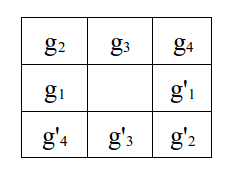
\includegraphics[width=0.2\textwidth]{./images/scov}
    \caption{A $3 \times 3$ neighborhood for center-symmetric pairs.}
    \label{figscov}
\end{figure}
\begin{equation}
	SCOV = \frac{1}{4}\sum_i^{4}(g_i - \mu)(g_i' - \mu)
	\label{scov}
\end{equation} 
Where: 
\begin{itemize}
	\item $g_i$: is grey-level of pixel $i$
	\item $g'_i$: is the grey-level of pixel that symmetric with pixel $i$
	\item $\mu$: is the local mean
\end{itemize}
\section{Features integration}
In most case, a single texture feature is not enough information to present for amount and spatial of local texture. The better way is considering the combination between two or more features. As an example, Lowe \cite{lowe2004distinctive} considered the use of gradient magnitude and direction to detect the dominant point in the image; Timo Ojala et al \cite{ojala1996comparative, ojala1999unsupervised} used LBP/Contrast and LBP/SCOV to classify the texture in the image.
\section{Local features and landmark estimation}
In this section, we show a way to combine the local features and evaluate the correctness of them for estimating the landmark on beetle's pronotum. Local binary pattern (LBP) and contrast(C) have been selected.\\
By using two images (source and target image) and their manual landmarks, method shows the way to evaluate the landmarks on the others. It includes two steps: (1) create the texture descriptor; (2) compare the similarity among the descriptors. Each landmark of the source image will be evaluated with all the landmarks of the target image.

For each manual landmark, a patch centered at the landmark is created  with size $s$. Then, for each pixel in the patch, a $3 \times 3$ neighborhood (Fig. \ref{figlbpc}a) is used to calculate the LBP and contrast. The original $3 \times 3$ patch is thresholded by the value of the center pixel (Fig. \ref{figlbpc}b). The values of the pixels in the thresholded neighborhood are multiplied by the binomial weights given to the corresponding pixels(Fig. \ref{figlbpc}c). The LBP of texture unit is summed of all obtained values (Fig. \ref{figlbpc}d). The contrast of the texture unit is defined as the difference between the average gray-level of the 1-pixels and 0-pixels. The contrast then is mapped from the continuous value to the discrete value by quantization. The pair LBP/C after that is presented into a two-dimensional accumulator of size $256 \times b$, where $b$ is number of discrete contrast. The process is continued until all pixels in the patch are considered.\\
\begin{figure}[htb]
    \centering
    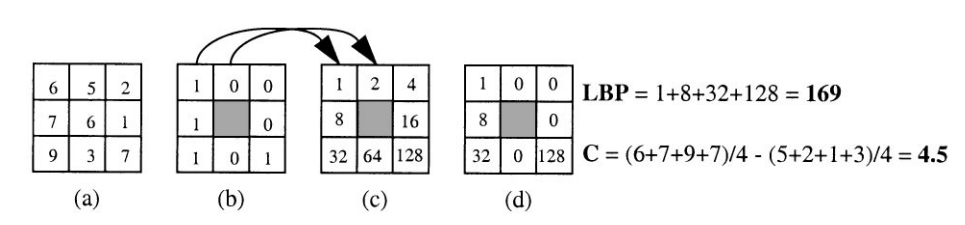
\includegraphics[width=0.9\textwidth]{./images/lbpc}
    \caption{LBP and contrast (C) computing.}
    \label{figlbpc}
\end{figure}
The comparing between the descriptors is done by using $L2$ distance.
\section{Result}
Timo Ojala et al \cite{ojala1999unsupervised} have proposed a method to segment the texture using LBP/C. The evaluation is done on Mosaic \#2 (a $512 \times 512$ image containing four texture made by a GMRF process). The segmentation error is 4.2\% error for the first sweep, it is quite decent. The final error is 1.2\% (after 23 sweeps); Mosaic \#3 (a $512 \times 512$ image with a background made by a GMRF process and four distinct regions) with final error is 1.9\% after 13 sweeps; Mosaic \#4, \#5 are composed of textures taken from outdoor scene. The segmentation errors are 3.3\% and 2.1\%, respectively. From this result, the combining between LBP and contrast could be a good pair for the classification application. An advantage of this method that it does not require any knowledge about how many texture or regions in the image.


In the context of combining the local features, we apply LBP/C to evaluate the effect of this feature pair on the texture around the landmark (as described before). The result shows that the distance of pair at landmark $3^{rd}, 4^{th}, 6^{th}, 7^{th}$ is better than other ones. This mean that the pair LBP/C is worked well on the pattern which have the distinctable pixels.

In another examine, the scene image is segmented by applying Canny algorithm. Then, a patch around each contour point is created. The descriptor is computed and compared with the descriptor of the manual landmark of the model. The process keep the point of the contour that has minimum distance with the manual descriptor. Following this way, the evaluation is done on all manual landmarks of model. The result of examination shows that this method can estimate the landmark at the position $3^{rd}, 4^{th}$, and in some case of landmark $6^{th}, 7^{th}$.
\section{Conclusion}
In this works, we have studied the local features and their combination. We have applied the LBP/C to examine the sensitive of this pair with on the gray-scale of pronotum image. In the next, we will try to evaluate the other pair of local features on pronotum such as LBP/SCOV.
%\bibliographystyle{unsrt}
%\bibliography{includes/localfeatures}
	\chapter{Dominant points}
In shape analysis, extracting features from the curves is an important step because in another way, we can re-construct the shape from the features. The term dominant points, also called as siginficant points, points of interest, corner points or landmarks is assigned to the points which have the high effect on boundary of object; their dectection is a very important aspect in contours methods because these concentrate the information of a curve on the shape.\\[0.2cm]
Dominant points can be used to produce a presentation of a shape contour for futher processing. The representation ...
In the content of this chapter, we will discuss about the methods to determine the dominant in digital image.\\[0.2cm]
There are many approaches developed for detecting dominant points and the methods can be classified into three groups follows:
\begin{itemize}
	\item Dectermine the dominant points using some significat measure other than curvature
	\item Evaluate the curvature by transforming the contour to the Gaussian scale space.
	\item Search for dominant points by estimating directly the curvature in the original image space.
\end{itemize}
\section{Hough Transform}
One of the challenges in image processing is detecting the characteristic of the object for recognition. Shape recognition is done by searching or detecting a class of simple geometric object such as line, curves in the image and comparing with the model. The matching score of the shapes is calculating by a measurement distance (such as Bhattacharyya). Instead of comparing between the geometric classes from the shapes, we can detect the presence of a shape in anther shape by searching each feature of the shapes. To sovle this problem, Hough Transform (HT)\cite{mukhopadhyay2015survey} is varied. At the beginning, HT\cite{vc1962method} is used to detect the line. It converts the space of parameters from x and y (coordinate of points in line) to space of slope and y-intercept of the line by voting process. For each object statisfying with equation of a line, it votes for the bin have correspondence slope and y-intercept. The set of bins is called the accumulator.
\subsection{Generalizing Hough Transform}
Until now, HT is still a good method for line detection or object recognition. But one of the weakness of HT is cannot determine the end points of the line segments. For this reason, the Generalized Hough Transform (GHT), introduced by Ballard\cite{ballard1981generalizing} is a generalization of HT to detect non-parametric curves. The process includes two phases: learning and recognition. In learning phase, a R-table is construct for model object. R-table is constructed based on the geometric information of each points in curves of object model with a reference point. The reference point can be arbitrary point in the model. Each row in R-table includes the gradient direction of each point which was chosen as index of table; and the polar coordinate values of each point. This mean that a gradient direction can be having many polar coordinate values. During recognition phase, an accumulator is created, called Hough Space. For each point in the scene object, finding the correspondce gradient direction in the R-table and voting at all the coordinate values. The peak in accumnulator is position of reference point of the model object in the scene object. And the peak value is equal to the number of boundary points of the object  when the model and the scene match perfectly.\\[0.2cm]
During recognition phase, the translation and rotation between model object and scene object is determine by principal component axis. Based on the curve points of the object, the centroid of each object is calculated. Then, the principal axis of each object is indicated. The translation between two objects is difference of two centroid points. The angle to rotate is the angle difference of two axes.\\[0.2cm]
When model and scene are matching, the dominant points (landmarks) of scene object is estimated from landmarks of model object by applying the translation, rotation from the centroid points. The last result is verifying by apply template matching (which will discuss as section \ref{template}).
\subsubsection{Result}
Using GHT to extract the landmarks on beetle is experiment on 287 images of right mandible of beetle. To compare the matching between the location of manual landmarks and estimated landmarks, the centroid size is compute for each set of landmarks.\\[0.2cm]
\begin{figure}[h!]
\centering
\subfloat[Model 28]{\label{figpca1}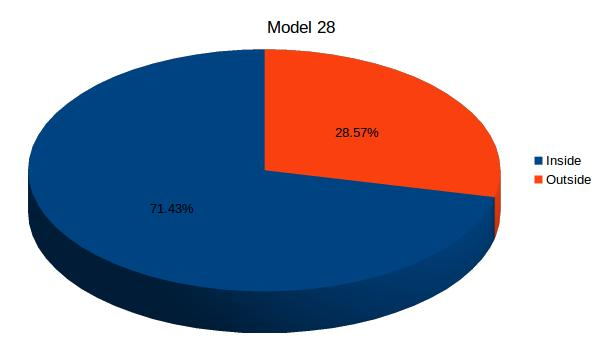
\includegraphics[width=0.5\textwidth]{./images/cmodel28}}~~
\subfloat[Model 71]{\label{figpca2}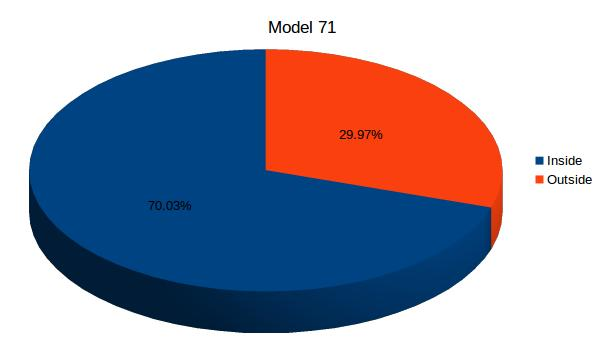
\includegraphics[width=0.5\textwidth]{./images/cmodel71}}
\caption{The accuracy of centroid size on mandible}
\label{figpca}
\end{figure}
Figure \ref{figcentroidSize} display the accuracy of the centroid size of estimated landmarks when we compare with the centroid size of manual landmarks. We use 2 images (Md28.JPG and Md71.JPG) as model. The number of landmarks be detected on scene object is 100\%. For model 28, 71.43\% the centroid of estimated landmarks is placed inside the standard deviation (SD) of manual landmarks, 28.57\% is outside the SD. The ratio for model 71 are 70.03\% and 29.97\%.
\subsection{Probabilistic Hough Transform}
To speed up Hough Transform, instead of processing on all data set, we can consider a subset of data points. The popular method is  \textbf{Probabilistic Hough Transform}. Probabilistic Hough Transform (PHT) is used to detect the presence of a model image in a scene image based on the group of features. The hypothesised location of the model image in the scene image is indicated based on the conditional probability that any pair scene lines agreement about a position in model image. Applying PHT can be separated into two steps: firstly, recording the information of model image and try to find the presence of the model image in scene image (called training process); secondly, predicting the pose of model image in the scene image (called estimating process).\\[0.2cm]
During training process, choose an arbitrary point in the model image, called reference point. For each pair of lines in model image, the perpendicular distance and angle from each line to reference point is recording (angle is calculated as angle between line and a horizontal line begin from reference point). The presence of model image in scene image is detected by PHT with \textit{``vote"} procedure. Finally, we choose the similar pair lines between model image and scene image. The chosen pair is obtained from best \textit{vote} when we consider each pair of line in scene image with each pair of lines in model image.\\[0.2cm]
In estimating process, the reference point in model image is estimated in scene image by extending the perpendicular lines of the pair of scene lines at the appropriate position. There, we can estimate the pose of the model in the scene image.

\section{Template matching}\label{template}
Template matching is a technique for finding areas of an image that match to a template image (template) by sliding the template over each pixel on the image (commonly cross-correlation). At each position, the sum of products between two images is calculated. The position is considered similar if the sum value at this position is maximal. The equation of cross-correlation is as follows:
\begin{equation}
\label{eq:cross-correlation}
	R_{ccorr}(x,y) = \sum\limits_{x',y'}[T(x'.y').I(x + x', y + y')]
\end{equation}
Where:
\begin{itemize}
\item T is template which use to slide and find the exist in other image.
\item I is image which we expect to find the template image
\item $(x', y')$ are coordinates in template where we get the value to compute.
\item $(x + x', y + y')$ are coordinates in image where we get the value to compute when template $T$ sliding.
\end{itemize}
However, if we use the original image to compute and find the similarity, the brightness of the template and the image might change the conditions and the result. So, we can normalize the image before applying the cross-correlation to reduce the effect of lighting difference between them. The normalization coefficient is:
\begin{center}
\begin{equation}\label{eq:normalizeCoff}
Z(x,y) = \sqrt{\sum\limits_{x',y'}T(x'.y')^{2}.\sum\limits_{x',y'}I(x + x', y + y')^{2}}
\end{equation}
\end{center}
The value of this method when we normalized computation as below:
\begin{center}
\begin{equation}\label{eq:cross-correlation}
R_{ccorr\_norm}(x,y) =\frac{R_{ccorr}(x,y)}{Z(x,y)} = \frac{\sum\limits_{x',y'}[T(x'.y').I(x + x', y + y')]}{\sqrt{\sum\limits_{x',y'}T(x'.y')^{2}.\sum\limits_{x',y'}I(x + x', y + y')^{2}}}
\end{equation}
\end{center}
\section{Image registration}
Image registration is process of transforming difference data sets into the same space and comparing or integrating the data from them. The object in image registration may be the images, time series or viewpoints. It is having many application in medical, military or satellites. In recent years, image registration is applied for both 2D and 3D objects with many methods. These methods may be classified following the characteristics of the input such as \textit{intensity-based and feature-based}, \textbf{transformation}, \textit{spatial and frequency},... In the context of this section, we want to discuss around the methods of linear transformations which include rotation, translation and scaling. Besides, we use these method to generate the general model from several objects or detect the landmarks on the object.
\subsection{Principal component analysis (PCA)}
Principal component analysis is computed based on principal directions of the datasets (model and scene). The input of this method is the list of points on curves of model and scene object (called model points and object points). The origin of the axes is centroid of all points on the curves. One of the axes is the line over the origin and having the minimum distance to all points in the curves; another axis is perpendicular axis with the first axis. The translation between two objects is different distance of centroid point coordinates; the rotation is different angle of two coordinate systems. The steps in PCA are followed:
\begin{itemize}
	\item Compute the centroid of model and scene object,
	\item Calculate the principal axes of model and scene,
	\item Compute the translation and rotation
	\item Translate the model to the scene that they have the same centroid.
	\item Rotate the model followed the different angle to match with the scene.
\end{itemize}
\subsubsection{Result}
The method is experiment with the set of right mandibles. Most of model can be detected its position on the scene by PCA. It also determine the translation and rotation information (see figure \ref{figpca1}). But in the case the input has more the noises, the centroid may be missed with correct position, following it is wrong translation and rotation(see figure \ref{figpca2}). In these examples, the red line is presented for the scene object and blue points is presented for the model object, which we want to align with the scene.
\begin{figure}[h!]
\centering
\subfloat[PCA with less noises]{\label{figpca1}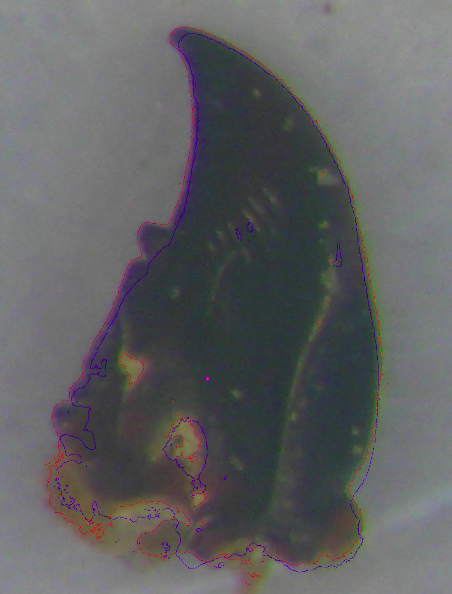
\includegraphics[width=0.3\textwidth]{./images/pca1}}~~
\subfloat[PCA with noises]{\label{figpca2}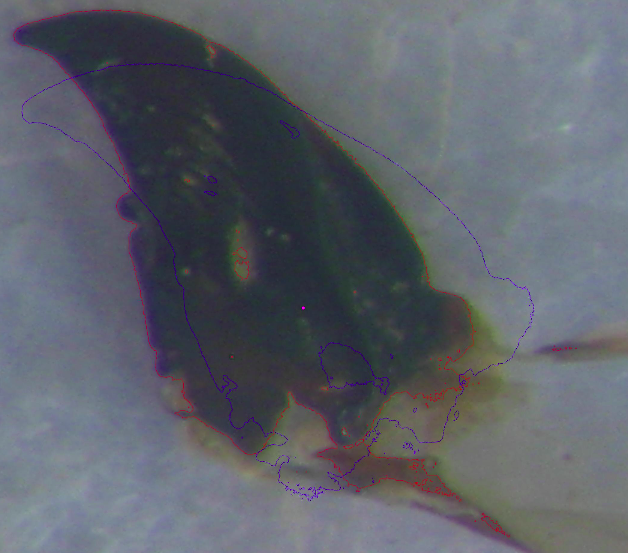
\includegraphics[width=0.4\textwidth]{./images/pca2}}
\caption{The result after applying the PCA}
\label{figpca}
\end{figure}
\subsection{PCA Iteration (PCAI)}
PCA method is a simplest method to align two images. However, PCA is more influenced by noises(see figure \ref{figpca}). Based on the idea of PCA method, PCAI try to apply the PCA on the interested data of the input.\\[0.2cm]
The solved problem in PCAI is the same with other difference registration methods. With two set of data input, specify curve points, we want to register two images with best matches. In PCAI method, firstly, PCA is applied on all two set of data for having the first sight of data. Secondly, the data is sorted followed one of coordinates of data points. The interested data is taken up with a half of data points which are sorted. Thirdly, an iteration will be executed to match the data. For each iteration, we re-compute the principal component of scene data and compare with the model. The iteration will be terminated when the difference position between two images is smallest (see figure \ref{figpcai}).\\[0.2cm]
\begin{figure}[h!]
\centering
\subfloat[Image alignment with PCA]{\label{figpcai1}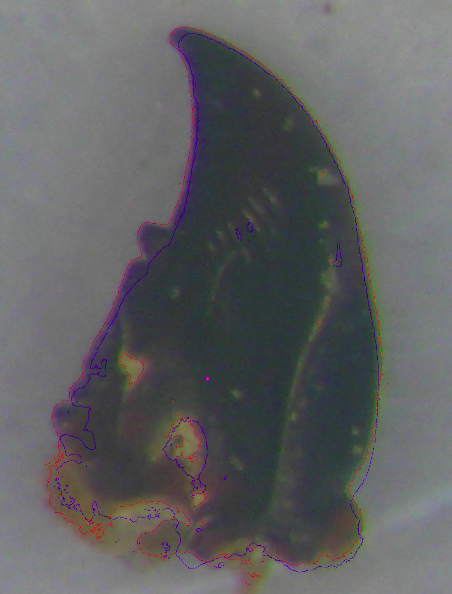
\includegraphics[width=0.4\textwidth]{./images/pca1}}~~
\subfloat[Image alignment with PCAI]{\label{figpcai2}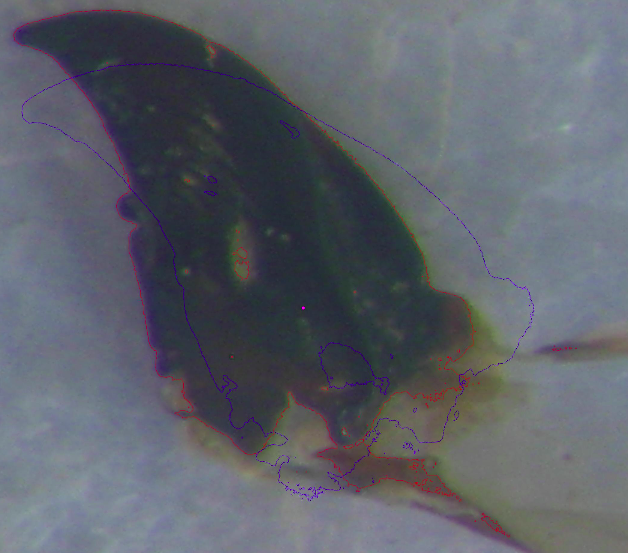
\includegraphics[width=0.4\textwidth]{./images/pca2}}
\caption{Comparing the result between PCA and PCAI}
\label{figpcai}
\end{figure}
Beside applying PCAI to make the images are matched. PCAI can combine with other technique to estimate the landmarks, such as template matching. At beginning, PCAI is applied to match the images. At the end, for each manual landmarks on the model, we apply the template matching to estimate the location of landmarks on scene image. 
\subsubsection{Result}
The combining between PCAI and template matching is experimented on two datasets of mandible (left and right mandible). For each set of data, it was divided into two sub-sets followed the size of objects. The model is chosen for each sub-set. The estimated landmarks coordinates are used to compute the centroid size of the mandibles. The results are compared with the centroid size of manual landmarks. In general, the success rate of the method is \textbf{90.56\%} for left mandible and \textbf{94.48\%} for right mandible (see figure...). On each sub-set of left mandible, the success rate of sub-set 1 is \textit{87.18\%} and \textit{97.80\%} for sub-set 2 (see figure). And \textit{94.52\%} and \textit{94.37\%} are success rates of sub-sets on right mandible(see figure).
Although the result from the method is good but it depends much on the result of segmentation. If the segmentation is not good and have many noises, the result of the method will be affected.
\subsection{Singular value decomposition (SVD)}
The PCA method is more effected by the noise, instead of using all the curve points, SVD just using a subset of points by optimal alignment between corresponding points of model and scene. Assume that \texttt{M} is a subset of the model points, \textbf{S} is a subset of the scene points and $p_i \in M, q_i \in S$ are two corresponding points. We would like to find the matrix transformed \textbf{R} so that the pair-wise distances between the corresesponding points is minimum. The pairwise distance is indicated by equation (\ref{eqpwdistance}).
\begin{center}
\begin{equation}\label{eqpwdistance}
	E = \sum_{i=1}^{n} {\|q_i - p_i^{'}\|}
\end{equation}
\end{center}
Where:
\begin{itemize}
	\item \textit{n}: is number of corresponding points
	\item \textit{$q_i$}: point of scene
	\item \textit{$p_i^{'}$}: point of model which corresponding with \texttt{$q_i$}
\end{itemize}
In detail, SVD method includes the following steps:
\begin{itemize}
	\item Calculate the cross covariance matrix: $M = P.Q^T$, where $P(Q)$ are matrix with i-th column is vector $p_i - c_T$ ($q_i - c_S$),
	\item Compute the singular value decomposition of matrix $M$: \textbf{$M = U.W.V^T$}. Where:
	\begin{itemize}
		\item U,V are \textit{m} x \textit{m} orthonormal matrices
		\item W is a diagonal \textit{m} x \textit{m} matrix with non-negative entries.
	\end{itemize}
	\item Indicate the orthonormal matrix (rotation matrix) $R = V.U^T$
\end{itemize}
\subsubsection{Result}
SVD method is solving the noise problem of PCA by using a set of corresponding points. The result obtained by applying the SVD also better PCA. But a disadvantage of SVD is requiring a accurate correspondences set of points which are usually not available.
\subsection{Iterative closest point (ICP)}
Based on the advantage and disadvantage of PCA and SVD. ICP combines two previous methods. The idea of ICP is using PCA to intial guess of correspondences and repeating SVD to improve correspondences. The steps of ICP are:
\begin{itemize}
	\item Transform the model by PCA aligment
	\item For each transformed model point, assign the closest scene point as its corresponding point. Align model and scene by SVD
	\item Repeat the step (2) until a termination criteria is met.
\end{itemize}
	\chapter{Software}
\section{The software architecture}
The architecture of program is followed 3-tier model. There-tier architecture is an architecture that each tier is designed, developed and maintained as independent. The advantage of this architecture is intended to allow any upgraded or replaced independent between the tiers. When user want to change the requirements or technology of a tier, it will non-affect to other tiers.\\[0.3cm]
The architecture of three-tiers includes:
\begin{itemize}
	\item \textbf{Data tier}: includes the classes which were designed for the data structure of program. It also provides the persistence mechanism to access the data.
	\item \textbf{Logic tier}: controls the functionality of application by performing detailed processing.
	\item \textbf{Presentation tier}: displays information related to user. It is a layer which received the require from user to program or return the result from program to user. 
\end{itemize}
\begin{figure}[h]
	\centering
	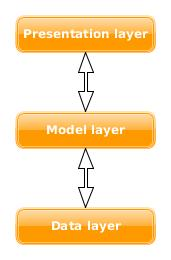
\includegraphics[scale=0.7]{images/software_3tiers}
	\caption{Three-tiers model}
	\label{fign3iters}
\end{figure}
\section{The modules}
The MAELab software mainly includes four modules: \textbf{segmentation}, \textbf{histograms}, \textbf{pht} and \textbf{correlation}. Besides, the software also includes the other modules to support for the main modules. The relation between the modules in the software is shown in figure \ref{fignsmodules}.
\begin{figure}[h]
	\centering
	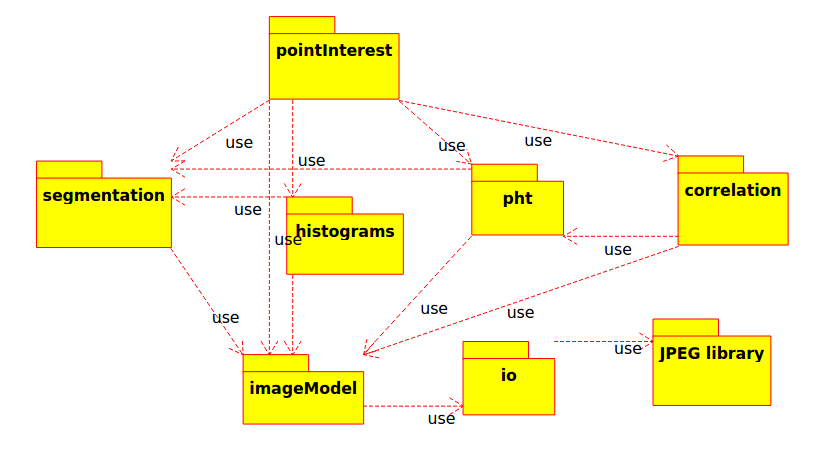
\includegraphics[scale=0.5]{images/modules}
	\caption{Three-tiers model}
	\label{fignsmodules}
\end{figure}
The functions of each modules is describing as followed:
\begin{itemize}
	\item \textbf{io} module: Implement the functions to read and write file. It includes the \textbf{JPEG library} that used to decode and encode the JPEG image.
	\item \textbf{imageModel} module: Represent the data structure of the image.
	\item \textbf{segmentation} module: Implement the segmentation methods on image.
	\item \textbf{histograms} module: Contains the methods to compute the geometric histogram of the image.
	\item \textbf{pht} module: Describe the probabilistic hough transform duration.
	\item \textbf{correlation} module: Includes the template matching methods.
	\item \textbf{pointInterest} module: Combine the result of the modules such as segementation, histograms,... to provide the adapter to other module or other software.
\end{itemize}
\section{The modules}
\section{The classes architecture}
\part{Deep learning}
	In the previous of thesis, we have studied the basic methods in image processing field. Then, the methods have been applied to determine the landmarks on biological images. They are known as the very well methods in image processing. In this part of thesis, we introduce another field that we have also applied to image analysis in recent years, that is machine learning, specially deep learning. 


Chapter 5 gives the principle context of machine learning. In this chapter, we present there problems of machine learning and we also give an overview about some machine learning algorithms.


Chapter 6 presents an sub-field of machine learning, \textbf{Deep Learning}. It displays an overview of deep learning problems. It has also present the convolutional neural network, a popular technique has been used in Deep Learning. At the end of the chapter, the libraries, which have been developed for Deep Learning, are also introducing.


Chapter 7 shows the applying of Deep Learing to predict the landmarks on biological images. This chapter presents the building process of the networks which have used to predict the landmarks. In this chapter also review some convolutional neural network, which have been employed to predict the facial keypoints.
	\chapter{Machine Learning}
Machine learning is a norm refer to teach the computer the abilities which are only done by the humans. A machine learning algorithm is an algorithm that is able to learn from data. Most of machine learning algorithms can be divided into two categories: supervised learning and unsupervised learning algorithms. \\
A machine learning algorithm is built based on the tasked for a machine learning system. We have many kinds of task can be solved with machine learning. Some of common machine learning tasks include the following:
\begin{itemize}
	\item \textit{Classification}: In this type of task, the computer is asked to indicate a category in k category which the input belongs to. To solve this task, the learning algorithm uses a function $y=f(x)$, the model assigns the input described by vector $x$ to a category identified by score y.
	\item \textit{Classification without input}: A challenge of classification is missing the input vectors. In this case, to solve the classification task, the learning algorithm only has to define a single function mapping from a vector input to a category output. When some of inputs are missing, instead of providing a single classification function, the learning algorithm must learn a set of functions. Each function corresponds to classifying x with different subset of its inputs missing.
	\item \textit{Regression}: the computer program is asked to predict a numerical value given some input.
	\item \textit{Transcription}: machine learning system is asked to observe a relatively unstructured representation of some kind of data and transcribe it into discrete, textual form.
	\item \textit{Translation}: The input already contains the sequence of symbols in some languages, the computer program must convert it into the sequence of symbols of other languages.
	\item \textit{Structure output}: involve any task where the output is a vector with important relationships between the different elements.
	\item \textit{Anomaly detection}
	\item \textit{Synthesis and sampling}: The program is asked to generate the new example that are similar with the training data.
	\item \textit{Imputation of missing value}: The algorithm mus provide a prediction of the values of the missing entries in a new example.
	\item \textit{Denoising}
	\item \textit{Density estimation or probability mass function estimation}
\end{itemize}
\section{Supervised learning algorithms}
\section{Unsupervised learning algorithms}
\section{Stochastic Gradient Descent}
	\chapter{Deep Network}
\section{Neural network}
\subsection{Neural}
The basic components of the brain is a neuron. For the ordinary man, we have billion neurons in the human nervous system, and they are connected by the billion of synapses. Each neuron receives input signals from its dendrites and procedures output signals along its axon.\\[0.2cm]
In the computational model of a neuron, the signals travel along the axons interact multiplicatively with the dendrites of the other neuron based on the synaptic strength at the synapse. The synaptic strength are learnable and control the strength at influence or inhibitory of one neuron on another. In basic mode, the input signals are summed and compared with a threshold value. If the sum is greater than threshold value, the neuron can fire, sending a spike along its axon. Actually, we have many firing rate (called activation function) at a neuron, and the common choice of activation function is the \textbf{sigmoid funciont $\sigma$}, because it take a real-valued input and squashes it to range between 0 and 1. The image () show the model of a neuron:
\begin{figure}[h]
	\centering
	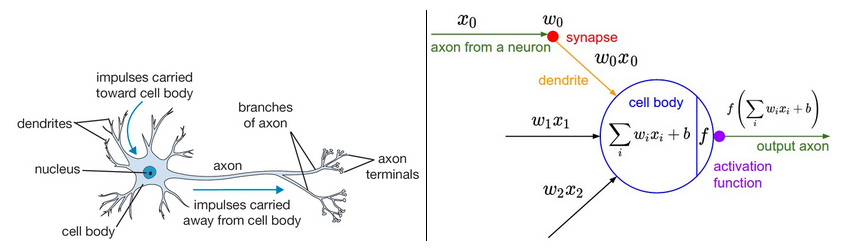
\includegraphics[scale=0.5]{images/neurons.png}
	\caption{A drawing of a biological neuron and its mathematical model}
	\label{fignneuron}
\end{figure}
Some activation functions which we can use:
\begin{itemize}
	\item \textbf{Sigmoid function}:
		\begin{equation}
			\sigma(x) = \frac{1}{1+e^{-x}}
		\end{equation}
	\item \textbf{Tanh}
		\begin{equation}
			tanh(x) = 2\sigma(2x) - 1
		\end{equation}
	\item \textbf{ReLU}
		\begin{equation}
			f(x) = max(0,x)
		\end{equation}
	\item \textbf{Maxout}:
		\begin{equation}
			f(w^Tx + b) = max({w_1}^Tx + b_1,{w_2}^Tx + b_2)
		\end{equation}
\end{itemize}
\section{The architecture of neural networks}
\begin{figure}[h]
	\centering
	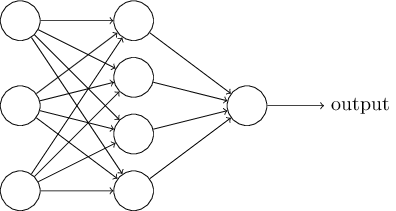
\includegraphics[scale=0.5]{images/neuron}
	\caption{A model of neural networks}
	\label{fignnnetworks}
\end{figure}
The image \ref{fignnnetworks} show a simple model of neural networks. The leftmost layer in this network is called the input layer, the rightmost layer is called the output layer. The neurons within the input layer are called input neurons, the neurons from output layer are called output neurons. The middle layer is called a hidden layer. The network in example \ref{fignnnetworks} has just a single hidden layer, but many networks have multiple hidden layers. When design the network, the input and the output are often straightforward. It means that the neural networks is designed where the output form one layer is used as the input to the next layer, there are no loops in the network, it always feed forward, never feed back (called feedforward networks).\\[0.2cm]
So, the neural network includes many layers are designed as an directred acyclic graph from the intput to the output layer. The output of previous layer is used as the input of the next layer. At each layer excepts the output layer, the output is indicated by a activation function (i.e loss, tanh,...). The size of a neural network can be to compute as the number of neurons, or the number of parameters.
\section{Deep network}
	\chapter{Classification}
Classification is a most of important task in machine learning. In classification, a function is constructed to determine the category of the input. Generally, the model of classification as following:

The process of classification includes two steps:
\begin{enumerate}
	\item \textbf{Training}: Use the \textbf{training set} to learn what every object of a class looks like. This duration is called training a classifier or learning a model. The training set is a set with the objects which have labeled with specific category.
	\item \textbf{Evaluation}: To evaluate the quality of the classifier. We use a new set \textbf{(test set)} of the objects and try to ask the classifier predict the category of the object in the test set.
\end{enumerate}
In the content of this chapter, we will discuss about the classification techniques, especially, linear classification which technique has used more in neural network and deep learning.
\section{Nearest Neighbour Classifier}
The first approach to Classifier, we will develop Nearest Neighbour Classifier. This classifier do not have any relation with deep learning or convolutional networks, but it will help us to have an overview about classification problem.\\[0.2cm]
The idea of Nearest Neightbour Classifier is comparing each image in test data set with all image in training data set and predict the label of closet training image. And one of simplest methods to compare two images is comparing each pixels of two images and sum of all the differences. Assum that we have two vector \textbf{$I_1$}, \textbf{$I_2$} presented for two images, the equation to compare two images is following (called \textbf{L1 distance}):
\begin{equation}
	d_1(I_1,I,2)=\sum_{p}|{I_1}^p - {I_2}^p|
\end{equation}
Actually, we have many ways to compute the distances between two image. Instead of using L1 distance, we can use \textbf{L2 distance}, which has indicated by square root of euclidean distance between two vectors. The form of L2 distance as: 
\begin{equation}
	d_2(I_1,I,2) = \sqrt{\sum_{p}{({I_1}^p - {I_2}^p)}^2}
\end{equation}
For example, this is a way to compute distace between two images  (fig. \ref{fignncl1}):
\begin{figure}[h]
	\centering
	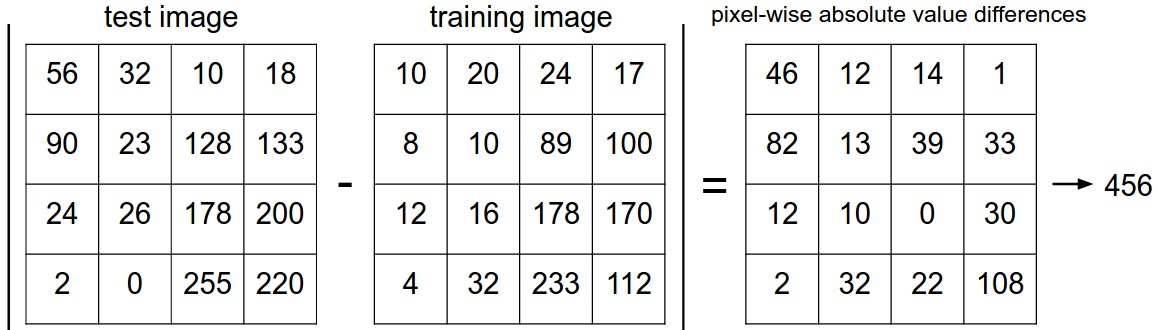
\includegraphics[scale=0.3]{images/nncl1.jpeg}
	\caption{An example used \textbf{L1 distance} to compare two images}
	\label{fignncl1}
\end{figure}
\section{K-Nearest Neighbour Classifier}
In the case of Nearest Neighbour Classifier, we just determine only one closest image in the training data with the test image when we wish to make a prediction. It means that we need some images in training data set that closest with the test image. In this case, we can use the \textbf{k-Nearest Neighbour Classifier}. The idea of this method is finding top \textbf{k} closest images instead of singel closest image (hence, when k = 1, we recover the Nearest Neighbour Classifier).\\[0.2cm]
In practice, what is the best value of k that we should to use? Besides that, we have many choices for  compute the distance between two images different with  L1 distance, L2 distance. The method called \textbf{hyperparameters} is vary for this work. This method comes in the design of many Machine Learning algorithsm, and it is used to choose the setting values. We should try out many different values and  see what works best. This is the idea, but we must be done vary carefully. Another noticed that, we do not try to evaluate on test data set with each \textit{k}. After having the \textit{k}, we evaluate on the test set only a single time, at the end of procedure.\\[0.2cm]
The idea is spitting the training data set in two subsets: the first subset is used to training, the other subset is used to validate (called \textbf{validation set}). The validation set is used as the test set to indicate the value of k. At the end of procedure, we could determine values of k work best. We would then use this value and evaluate once on the actual test set.\\[0.2cm]
In summary, split the training set into training set and validation set. use validation ton tune all hyperparameters. At the end run a single time on the test set and evaluate the result.
\section{Linear Classification}
The (k-)Nearest Neighbour Classifier had introduced about the problem of Image classification, which is predicting the label to an image from a fixed set of labels. But with the these methods, we must spend more time with large datasets an the cost for classifying is expensive. Another classification methods is known as \textbf{linear classification} which is the core of neural networks.
The linear classification has two main components: 
\begin{itemize}
	\item \textbf{Score function}:  which used to map the raw data to score of a category.
	\item \textbf{Loss function}: that quantifies the agreement between predict score and the truth category of the data.
\end{itemize}
The simplest function of a linear mapping is:
\begin{equation}
	y = f(x_i,W,b) = Wx_i + b
\end{equation}
Where:
\begin{itemize}
	\item $x_i$ is the raw data, \textit{example: an image}.
	\item $W$: a matrix parameter, called \textbf{weight} matrix
	\item $b$: vector, called \textbf{bias} vector
	\item $y$: score when consider the data $x_i$ belongs to a category.
\end{itemize}
In equation above, the input image \textbf{$x_i$} is fixed but we can control the setting of parameters \textbf{W and b}. Our goal is setting the parameters that the computing score match with the truth labels of image.
\begin{figure}[h]
	\centering
	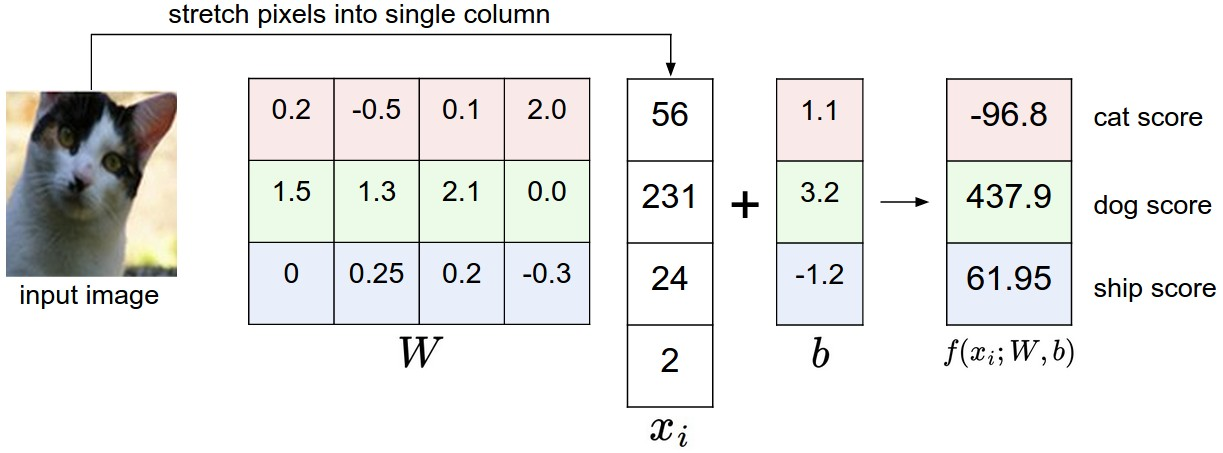
\includegraphics[scale=0.3]{images/lncex}
	\caption{An example of mapping an image to a class scores}
	\label{figlncex}
\end{figure}~\\
In training process, it is a little cumbersome to keep two sets of parameters (W,b) separately. A commonly trick is used to combine two sets of parameters into a single matrix that holds both of them by extending a vector \textbf{$x_i$} with one additional dimension and keep the constant defaut 1. Now, the new score function will be:
\begin{equation}
	y = f(x_i,W,b) = Wx_i
\end{equation}
Visualation of new score function:
\begin{figure}[h]
	\centering
	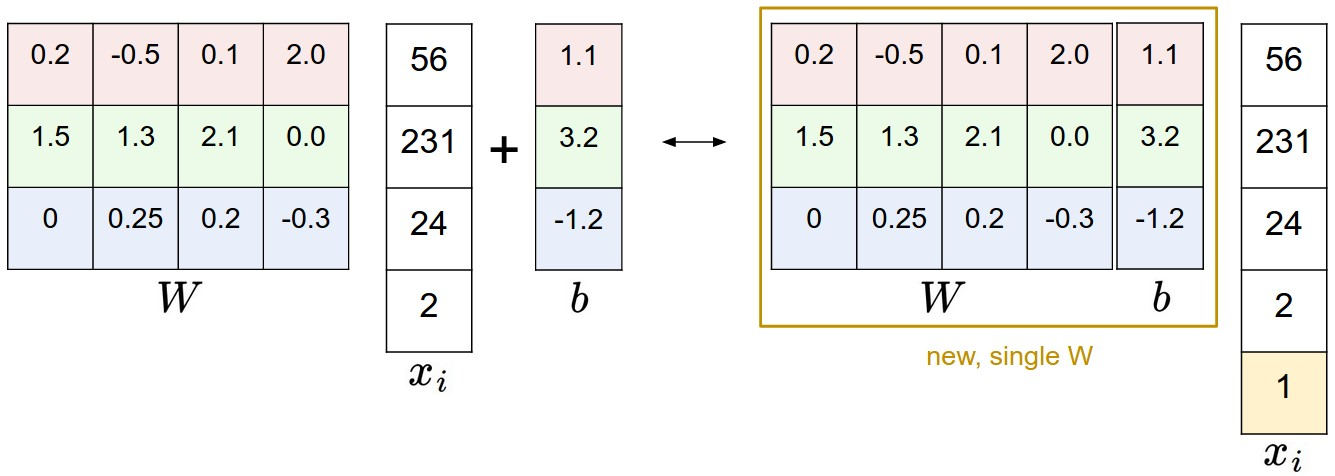
\includegraphics[scale=0.3]{images/lncba}
	\caption{An example of bias trick}
	\label{figlncex}
\end{figure}~\\
As described, we defined a score functions from a pixels value of an image to class scores with set of parameters \textbf{W}. Moreover, we need to control over parameters W such that the class scores are consistent with the ground truth labels in the training data. But not all cases are perfect, the class scores just near with the score of truth labels. So, we are going to measure the wrong with a \textbf{loss function}. Intuitively, the loss will be high if we are doing a poor classifier, ant it will be low if we are doing well. Multicalss Support Vector Machine (SVM) and Softmax function are two commonly methods for this purpose.
\subsection{Multiclass Support Vector Machine loss}
A commonly way to define the loss function called the \textbf{Multiclass Support Vector Machine} (SVM) loss. SVM loss is set up a margin $\Delta$ for the incorrect class scores. It means that SVM loss function wants the score of the correct class to be greater than the incorrect class (predict score) by at leat $\Delta$. If this is not the case, we will accumulate the loss.\\[0.2cm]
The SVM loss for the i-th is formalized as follows:
\begin{equation}
	L_i = \sum_{j \neq y_i }max(0,s_j - s_{y_i} + \Delta)
\end{equation}
Where:
\begin{itemize}
	\item $s_j$ is the score of $x_i$ for j-th class
	\item $s_{y_i}$ is the score of correct class
	\item $\Delta$ is margin 
	\item $max(0,-)$ is thresholding to zero, called hinge loss.
\end{itemize}
For example, we have three predict scores of an image $x_i$ like \textbf{$s = [14,-9,11]$}, and the first class is true class of $x_i$. Assume that $\Delta$ is 10. The SVM loss of this case is following:
\begin{center}
$
	L_i = max(0,-9 - 14 + 10) + max (0,11 - 14 + 10) = 0 + 7 = 7
$
\end{center}
\subsection{Softmax classifer}
The other popular choice to define the loss function  is the \textbf{Softmax classifier}. Unlike SVM which treats the output of score function for each class, the Softmax classifier give a sightly more intuitive output and use the probabilistic description. Instead using theshold zero function as SVM, Softmax is using a \textbf{cross-entropy loss} for \textit{hingle loss}, which has the form.
\begin{equation}
	L_i = -log(\frac{e^{f_{y_i}}}{\sum_j{e^{f_j}}})
	\label{softmax}
\end{equation}
Where: $f_j$ is the j-th element of vector of class scores \textbf{$f$}.\\[0.2cm]
In formula \ref{softmax}, the function $f_j(z) = \frac{e^{z_j}}{\sum_k{e^{z_k}}}$ is called the softmax function. This formula turns the predict scores into probabilistic values (Noticed that sum of all \textbf{$f_j(z) $} is 1).\\[0.2cm]
The cross-entropy between a correct distribution \textbf{p} and an estimated distribution \textbf{q} is defined as:
\begin{equation}
	H(p,q) = -\sum_x{p(x)log(q(x))}
\end{equation}
The Softmax classifier is minimizing the cross-entropy between the estimated socre and true score. At the end, the loss of training process is the average of cross-entropy.
\begin{equation}
	L = \frac{1}{N}\sum_i(H(p,q))
\end{equation}
The image \ref{figsvmsf} describes an example for a comparison between SVM and Softmax:
\begin{figure}[h]
	\centering
	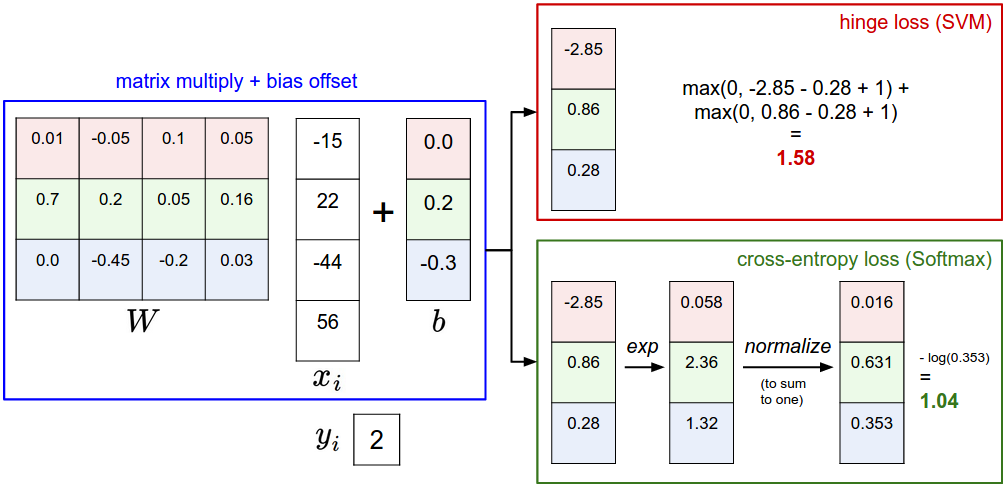
\includegraphics[scale=0.45]{images/svmsf}
	\caption{An example about SVM and Softmax classifiers}
	\label{figsvmsf}
\end{figure}~\\[2.5cm]
Both SVM and Softwax compute the same score of vector f. The difference is the way to present the score f: SVM uses the margin and Softmax uses probabilistic. In practice, the SVM and Softmax are usually used and compared in the machine learning systems.
\section{How to determine the value of W and b?}
\section{Backpropagation}	
	\chapter{Convolutional Neural Network}
Convolutional Neural Networks (CNNs) are similar with the original of Neural Networks. Neural Networks receive an input and pass it through a series of hidden layer. Each hidden layer is made from a set of neurons, where each neuron is full connected with all neurons of previous layer. Actually, the neural networks do not scale well to full images...
\section{Architecture}
A CNN is made from the layers. The common layers in CNN are convolutional, nonlinear, pooling and full connected layers. CNN takes image as an input, pass it through the series of layers and get an ouput. Each layer has a difference function to transform the input to another layer. 
\subsection{Convolutional layer}
\subsection{Pooling layer}
\subsection{Full connected layer}
\section{Testing}
	\chapter{Using CNN to classify the patches}
Deep learning powers computer vision with processing the data in high level such as image, sound, video in many tasks: classification, recognition or object detection. 
As a result of studying about the CNN, in this chapter, we proposed a model to classify
the landmarks on the pronotum of beetle. For each landmark in pronotum image, a patch
has been extracted with the size of $63\times63$. Then, the patches are used as the input of the model to train. At the end, a number of patches are tested to evaluate
the prediction of the model.

\section{Data}
The pronotum dataset includes 293 images. For each image, a set of 8 landmarks have been set manually by the biologist. For each landmark, a patch is extracted with the size of $63\times63$.
The images have been divided into 3 sets: training set included 200 images ($200 \times 8 = 1600 $ patches), validation set had 60 images ($60 \times 8 = 480$ patches) and 33 images ($33 \times 8 = 264$ patches) belong to the test set.

To evaluate the efficient of the network, the data has been chosen followed 3 ways: 
\begin{enumerate}
	\item In the first way, 200 first images are used as training data; next, 60 images are used as the validation data; and the test is remaining images.
	\item In the second way, 33 first images are chosen as test data; next, 200 and 60 images are chosen as training and validation data, respectively.
	\item In the last way, the images are divided randomly into 3 sets with the corresponding quantity.
\end{enumerate}

Besides, the patch's size also changed to find the suitable size for the patch for each landmark: $27 \times 27$, $45 \times 45$ and $63 \times 63$. The network trained with two types of the images: grayscale and RGB color.
\section{The network}
We propose a CNN-based method to classify the landmarks on the pronotum (see Fig. \ref{figCNNclassify}). The input of the network is the patches around the landmarks. The network includes three convolutional (CONV) layers followed by three pooling layers (maximum and average pooling) and two full connected layers. 
\begin{figure}[h]
	\centering
	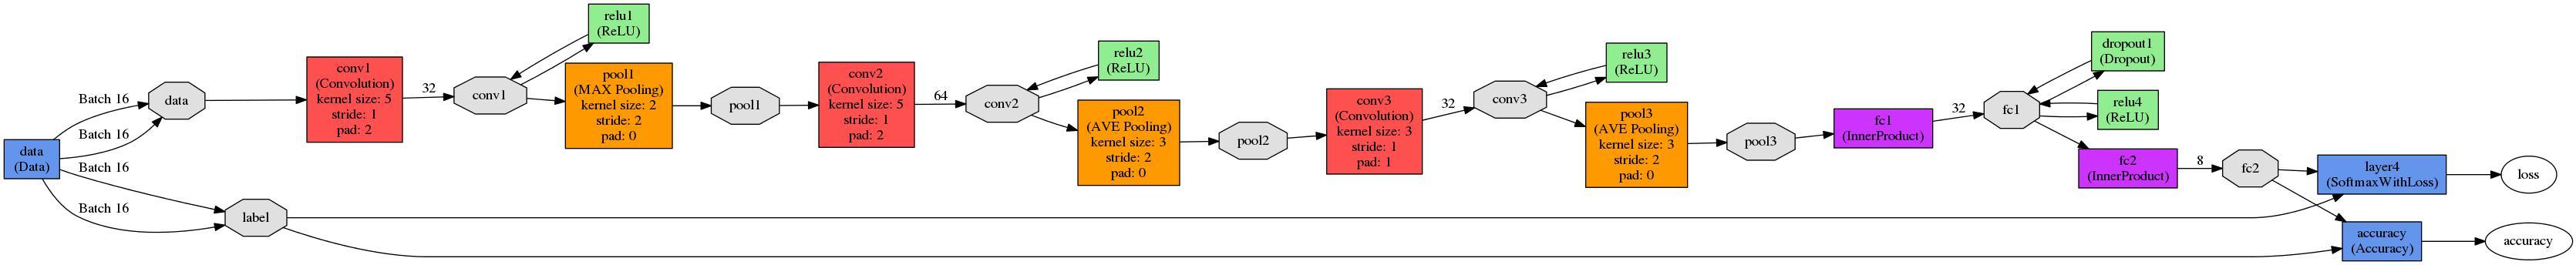
\includegraphics[scale=0.2]{images/CNN_classify}
	\caption{CNN model architecture}
	\label{figCNNclassify}
\end{figure}

The number of convolution filters are 32, 64 and 32, respectively. The window size of those filters are $5\times5, 5\times5$ and $3\times3$. For each CONV layer, a Rectifier Linear Unit is add to introduce the non-linearity for CNN.

Followed each CONV layer is a pooling (POOL) layer. The POOL layers with stride of $2\times2$ is reducing the computation for the deeper layers. The first fully connected (FC) layer consists of 32 neurons. To reduce the risk of the over-fitting on the network, a dropout layer is followed the first FC. The second FC layer output 8 values corresponding to 8 classes of the landmarks. Finally, a softmax with loss layer and accuracy layer are placed at the last stage of the network.
\section{Solver parameters}
The network is trained in $100000$ iterations. For each $10000$ iterations, a test phase will be executed in $1200$ iterations to validate the accuracy of the network.
During training, the Stochastic Gradient Descent (SGD) is used to update the value for learnable parameters. At the beginning, the learning rate is set to $0.0001$, after each $22000$ iterations, the learning rate is dropped as $10^{-3}$. Besides, $90\%$ value of previous computation will be retained in the new calculation.
\section{Experiment and results}
The network is trained with the data that chosen in three ways. In each way, two kinds of datasets are used: color patches and grayscale patches. For each dataset, three patch's size is used to prepare the data: $27\times27$, $ 45\times45$ and $63\times63$. The accuracy of the network on each dataset is provided in the tables following:
\begin{table}[h]
	\centering
	\begin{tabular}{{l}*{3}{c}}
		
		Size of patches &  $27 \times 27$ & $ 45 \times 45$ & $63 \times 63$  \\ \hline
		Accuracy on color patches & 73 & 83.14 & 88.97 \\ 
		Accuracy on grayscale patches & 57.25 & 72.08 & 77.91 \\ 
		\hline
	\end{tabular}
	\caption{The accuracy of the model on the data that chosen by the first way.}
	\label{tb1}
\end{table}

\begin{table}[h]
	\centering
	\begin{tabular}{{l}*{3}{c}}
		
		Size of patches &  $27 \times 27$ & $ 45 \times 45$ & $63 \times 63$  \\ \hline
		Accuracy on color patches & 75.193 & 85.417 & 89.168 \\ 
		Accuracy on grayscale patches & 64.385 & 72.11 & 78.1077 \\ 
		\hline
	\end{tabular}
	\caption{The accuracy of the model on the data that chosen by the second way.}
	\label{tb2}
\end{table}

\begin{table}[h]
	\centering
	\begin{tabular}{{l}*{3}{c}}
		
		Size of patches &  $27 \times 27$ & $ 45 \times 45$ & $63 \times 63$  \\ \hline
		Accuracy on color patches & 77.286 & 87.751 & 89.979 \\ 
		Accuracy on grayscale patches & 64.163 & 76.455 & 82.709 \\ 
		\hline
	\end{tabular}
	\caption{The accuracy of the model on the data that chosen by the third way.}
	\label{tb3}
\end{table}
As the result shown in three tables (table. \ref{tb1}, \ref{tb2}, \ref{tb3}), it seems that the network did not have more sensitive with the way to choose the data. But we have the different result from color and grayscale patches and the result is also improved when we increase the size of the patches from $27\times27$ to $63\times63$.

From the accuracy of training on each dataset, the patches of size $63\times63$ which selected by randomly are used to predict. The prediction is run on $33$ images ($33 \times 8 = 264$ patches). The label of a patch is label with highest prediction. Table \ref{tb4} shows the statistic of prediction on the dataset. Followed that, most of the landmarks are predicted with high accuracy ($\geq 78\%$). The proportion on $5^{th}$ landmark is not hight and it has a confusion with the $1^{st}$ landmark.
\begin{table}
	\centering
	\begin{tabular}{*{9}{c}}
		& LM 1 & LM 2 & LM 3 & LM 4 & LM 5 & LM 6 & LM 7 & LM 8 \\ \hline
		LM 1 & 87.88\% & 	6.06\% &	 0.00\% &	0.00\% & 	0.00\% & 	0.00\% & 	0.00\%	& 6.06\% \\ \hline
		LM 2 &	6.06\% &	 	90.91\% &	3.03\% & 	0.00\% & 	0.00\% & 	0.00\% & 	0.00\% & 	0.00\% \\ \hline
	LM 3 &	0.00\% & 	3.03\% & 	87.88\% &	3.03\% & 	0.00\% & 	0.00\% & 	6.06\% & 	0.00\% \\ \hline
	LM 4	 & 9.09\% &	0.00\% & 	6.06\% & 	81.82\% &	0.00\% & 	0.00\% & 	3.03\% & 	0.00\% \\ \hline
	LM 5	 & 51.52\% &	0.00\%	& 0.00\%	 & 9.09\% &	39.39\%	& 0.00\%	 & 0.00\% &	0.00\% \\ \hline
	LM 6	 & 12.12\%	& 3.03\%	 & 0.00\% &	0.00\% & 	0.00\% & 	81.82\% &	0.00\% & 	3.03\% \\ \hline
	LM 7	 & 3.03\%	& 0.00\%	 & 9.09\%	& 0.00\%	 & 0.00\%	& 0.00\%	 & 84.85\% &	3.03\% \\ \hline
	LM 8	 & 18.18\%	& 0.00\% &	0.00\%	& 0.00\%	 & 0.00\%	& 0.00\% &	3.03\% &	78.79\% \\ \hline

	\end{tabular}
	\caption{The prediction accuracy on the color patches of size $63\times63$}
	\label{tb4}
\end{table}
\section{Conclusion}
In the content of this work, a model in CNN is proposed to predict the class of the landmarks on pronotum. The network consist 8 layers: 3 CONVs, 3 POOL, 2 FC. For each landmark, the patches with different size are extracted to use as the input data of the model. The experiment shown that the model is worked well on the color batches with larger size. However, a confusion also exists when the model try to predict $5^{th}$ landmark.
	%\chapter{Deep Learning Frameworks}
Along with the deep learning methods in several domains, the deep learning frameworks have been developed to support the implementation. This chapter  presents several deep learning frameworks such as Caffe, Theano, TensorFlow, Torch, PyTorch,.... Besides, a comparison of 3 deep learning frameworks: Caffe, Theano, TensorFlow is studied. The study is detailed on two networks: AlexNet\cite{•} and a proposed network. The information that we want to study are not the speed, hardware utilization or extensibility; instead of, we want to know how the parameters effect to the result during training and choose the best framework for the next study. The comparative study of the frameworks is done on the CIFAR-10 dataset \cite{•} and the dataset of patches around the landmarks on the pronotum. 
\section{Deep learning frameworks}
Deep learning is more and more popular in many application domains over the last few year, there have a lot of laboratory (...) and industry group (Google, Facebook, Amazon) to develop the software frameworks. That thing is help easily to create and test the neural networks. At this time, many frameworks have been proposed for deep learning (see the complete list of deep learning software at DeepLearning.net \footnote{$http://deeplearning.net/software\_links/$} or DeepLearing4j.org \footnote{$https://deeplearing4j.org$}). In this section, we represent the main character of some of the widely used software frameworks: Caffe, Theano, TensorFlow, Torch; and the frameworks that used for other domain than computer vision, such as DyNet, DSSTNE.
\subsection{Caffe}
Caffe\cite{•} is a deep learning framework for computer vision. It is developed by Berkey AI Research (BAIR)\footnote{site} and community contributors. Caffe is written in C and C++. Besides providing a API on C++, it also provide the API on Python. Caffe is used by a large community of deep learning. Most of application which deployed in Caffe is processed on images. Caffe supports the train and test on both CPU and GPU.

\subsection{Theano}
Theano\cite{•} is a Python framework which developed by MILA lab at University of Montreal.It allows the user define, evaluate the convolutional neural network. With the purpose optimizes the 
compiler, Theano combines aspects of computer algebra system (CAS) which is particularly useful for the repeated tasks. Like Caffe, Theano is also providing the execution the network by CPU or GPU.
\subsection{TensorFlow}
TensorFlow\cite{•} is an open source software library for numerical computation using data flow graphs. Each node in the graph represents for a mathematical operation, while the edge represents the communication between the data arrays(tensors). Tensorflow supports Python and C++, along to allow computing distribution among CPU, GPU and even horizontal scaling.
\subsection{Torch}
Torch \cite{•} is a scientific computing framework for machine learning. It is written by Lua language. Torch 
\subsection{PyTorch}
\section{Experiments}
Table. shows the number of users of each frameworks in recently years.
Table. shows the properties of the deep learning frameworks. According the table, we have compared on some popular properties of a framework such as programming language core, training support devices (CPU, GPU), multi CPU (GPU) supporting, \ldots

To have a conclusion about the performance of the frameworks, we have set up on a single machine running on Ubuntu ....  For Caffe, version xxx is installed. For Theano and PyTorch, version xxx and yyy are used, respectively.

The experiments are done on two famous datasets: MNIST \cite{} and CIFAR-10 \cite{}. 
\subsection{MNIST dataset on Caffe and Theano}
\subsection{CIFAR-10 dataset on Caffe and Theano}

\section{Result and discussion}
	\chapter{Deep learning datasets for landmarking}
In deep learning, the dataset is a most of important field that "gop phan" to the success of deep learning. The collections the data is depend on the field of project. This chapter presents the deep learning datasets, specially, the biological datasets for landmarking detection in 2D images. 
\section{Facial keypoints problem}
In this section, we will present the datasets that have been built for detecting the keypoints (landmarks) on human face.
\subsection{CASIA WebFace}
Dong Yi et al. [] have proposed a semi-automatical way to collect the face images from Internet\footnote{http://www.cbsr.ia.ac.cn/english/CASIA-WebFace-Database.html}. The dataset includes 10575 subjects and 494414 images. Based on the database, a $11-$layers CNN was trained to illustrate the quality of the images. The accuracy was compared with the state of the art methods, such as: \textit{Deep Face, DeepID2}. (can not download)

\subsection{The Annotated Facial Landmarks in the Wild dataset}
Annotated Facial Landmarks in the Wild (AFLW) \cite{koestinger11a} is a dataset of annotated face images gathered from Flickr. The images recognize the human face with difference  information such as, pose, expression, age, gener. In total, AFLW contains 25000 annotated face images with up to 21 landmarks per image. This database is public at AFLW site\footnote{https://www.tugraz.at/institute/icg/research/team-bischof/lrs/downloads/aflw/}.
\subsection{Multi-Task Facial Landmark (MTFL) dataset}
Multi-Task Facial Landmark (MTFL) has been trained on the same database with \cite{sun2013deep}. It includes $5590$ LFW images, $1521$ BioID images, $781$ LFPW training images, $249$ LFPW test images and $7876$ other images dowloaded from the web. The images have been divided into training ($13466$ images) and testing set ($2552$ images). During training, each face in the image is labeled with five key points. 
\subsection{Facial Keypoints Detection Kaggle Challenge}
The dataset has been built for a challenge of facial keypoints detection. It includes two sets of images: training set contains $7049$ images; testing set includes $1783$ images. The size of images in the dataset was kept as $96 \times 96$ pixels. All the information of images has been saved into \textit{CSV} files. In training set, each row of CSV file contains the coordinates $(x,y)$ for 15 key points and the image data as row ordered list of pixels. In testing set, each csv row contains the image identification and image data as row ordered list of pixels. The dataset has been published at Kaggle website\footnote{https://www.kaggle.com/c/facial-keypoints-detection/data}.
\section{Other problems}
\subsection{Syntheseyes dataset}
Erroll Wood et al \cite{wood2015_iccv} proposed synthesizing perfectly labelled photo-realsitic training data in a fraction of the time. The eye-regions models have been built from head scan geometry by using computer graphics techniques. The models were randomly posed to synthesize close-up eye images for a wide range of head poses, gaze directions and illumination conditions. For each image, each 3D eye-region landmarks with 28 landmarks have been set manually, corresponding to the eyelids (12 landmarks), iris boundary (8 landmarks), and pupil boundary (8 landmarks).
The database is exists at SynthesEyes\footnote{https://github.com/danakianfar/landmark\_detection}.
\subsection{Lip reading dataset}
Note \footnote{http://www.robots.ox.ac.uk/$\%$7Evgg/data/lip\_reading/}
\section{Summary}
The summary of alldatasets are shown in the following table:\\
\begin{table}[!h]
	\centering
	\begin{tabular}{*{5}{c}}
		Name of databse & N$^{o}$ images & Size of image & N$^{o}$ landmarks & Project \\ \hline
		MTFL & $16018$ & $x \times x$ & 5 & No \\ \hline
		FKDKC & $8832$ & $96 \times 96$ & 15 & Challenge \\ \hline
		SynthesEyes & $11382$ & $120 \times 80$ & 28 & Yes \\ \hline
		LRS & $11382$ & $120 \times 80$ & 28 & Yes \\ \hline
	\end{tabular}
	\caption{The summary of deep learning datasets}
	\label{tb4}
\end{table}

	\chapter{Automatic extraction the morphometry landmarks by Convolutional Neural Network}
In the content of this chapter, we studied on the articles: \textbf{Deep Convolutional Network Cascade for Facial Point Detection}\cite{sun2013deep} (Yi Sun et al) and \textbf{Automatic ear detection and feature extraction using Geometric Morphometrics and Convolutional neural networks}\cite{cintas2016automatic} (Celia Cintas et al). Both of articles proposed the specific to automatic identification the landmarks on human face and human ears. Besides the studying, we also tried to apply the networks to estimated the landmark on the pronotum dataset \cite{}.
\section{Facial Point Detection by CNN}
Yi Sun et al proposed a method to estimate the position of five facial keypoints: left eye center, right eye center, nose tip, left mouth corner and right mouth corner (called landmarks). The proposed method includes 3-levels designed convolutional networks.
\subsection{Data}
The dataset with 13466 face images includes 5590 images from LFW \cite{huang2007labeled} and remaining images are downloaded from the web. The dataset is divided into training set with 10000 images and validation set with 33466 images. Each face is labeled with five landmarks and bounding box is created around the face. It was used as the input at the F1 network of the first level. At other networks, the bounding boxes are also used to limit the training region but with different size.
\subsection{Model}
\begin{figure}[h]
	\centering
	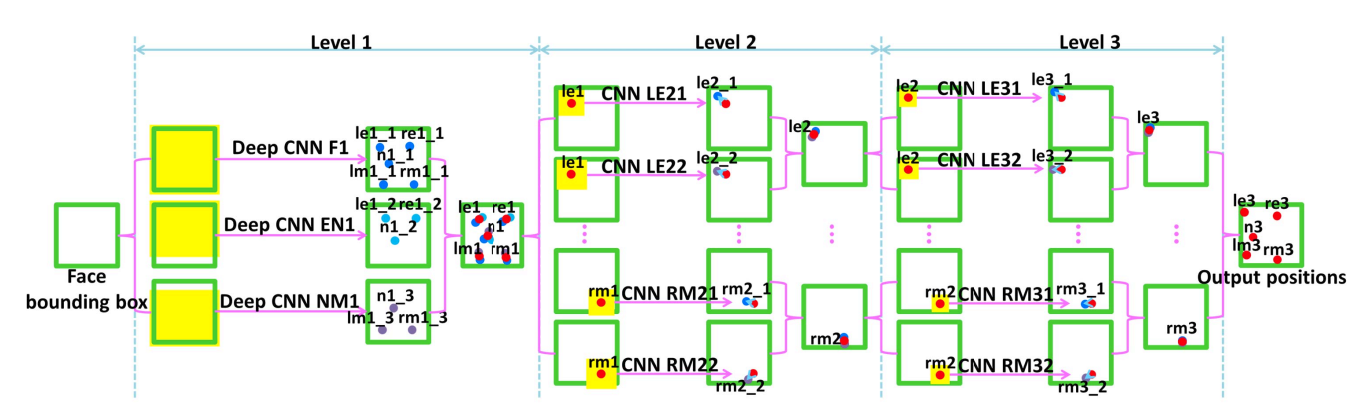
\includegraphics[scale=0.3]{images/3levels}
	\caption{The 3-levels proposed architecture}
	\label{3levels}
\end{figure}
They cascade three levels of convolutional networks to make the prediction (Fig. \ref{3levels}). The first level in architecture is designed to detect multiple landmarks, two last levels are designed to verify the position of each landmark.

At the first level, three CNNs are employed to study the location of the facial points: F1, EN1, NM1 whose input regions cover the whole face (F1), eyes and nose (EN1), nose and mouth (NM1). Each network predicts the landmarks corresponding with the region that it covers. At the end of level 1, the coordinate of each landmark is average of coordinates that predicted from three networks.
\begin{figure}[h]
	\centering
	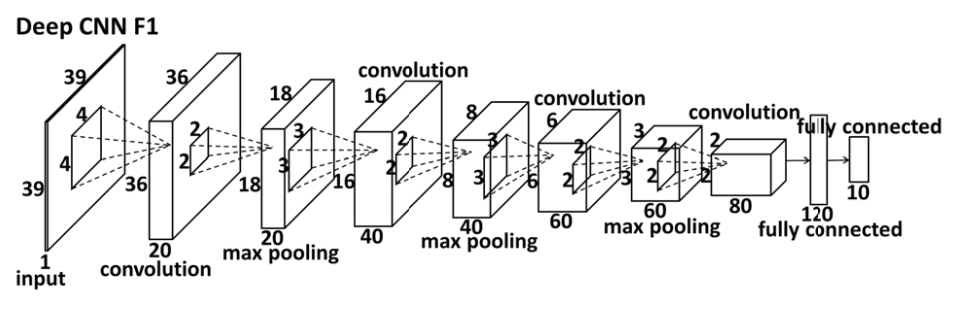
\includegraphics[scale=0.3]{images/1Fconv}
	\caption{The structure of F1-convolutional network}
	\label{1Fconv}
\end{figure}
Fig. \ref{1Fconv} illustrates the deep structure architecture of F1 network, which contains four convolutional layers followed by max pooling and two full connected layers. The structure architecture of EN1 and NM1 are also the same with the structure of F1. The only difference is the different size at each layer because the size of the input regions are different.

The networks at the second and third levels take local patches centered at the predicted position of previous levels as input and are allowed to make small changes to previous prediction. The size of patches are also reduced along with the cascade model. For each position, two networks are used to predict the new positions and the last predicted position is average of the new positions. With 3-levels model, the purpose of the networks at the first level are estimated the landmark positions with large errors; the networks at last two levels are designed to achieve high accuracy.
\subsection{Experiments}
\subsubsection{Training}
At the first level, the patches according the bounding boxes are used as the input of the networks. At the following levels, the patches centered at previous predicted position is used to train. The size of the patches is decreased for each level. The learnable parameters include weight w, the gain g and the bias b which are initialized by small random number and learned by stochastic gradient descent.

The detection error on each facial point is measured by Eq. \ref{eq1}. If the error is greater than $5\%$, it is considered as failure.
\begin{equation}
	err = \sqrt{(x-x')^2 + (y-y')^2}/l
	\label{eq1}
\end{equation}
Where:
\begin{itemize}
	\item l is the width of the bounding box around the face.
	\item $(x,y)$ is ground truth facial point
	\item $(x',y')$ is predicted position
\end{itemize}
\subsubsection{Testing}
The model is tested with a dataset of 2557 face images. The image with the bounding box of the face is used as the input of the model. At the end, the predicted position is estimated from the model. By using the way in Eq.(\ref{eq1}) to evaluate the model, the error statistic on each level is obtained.
\begin{figure}[h]
	\centering
	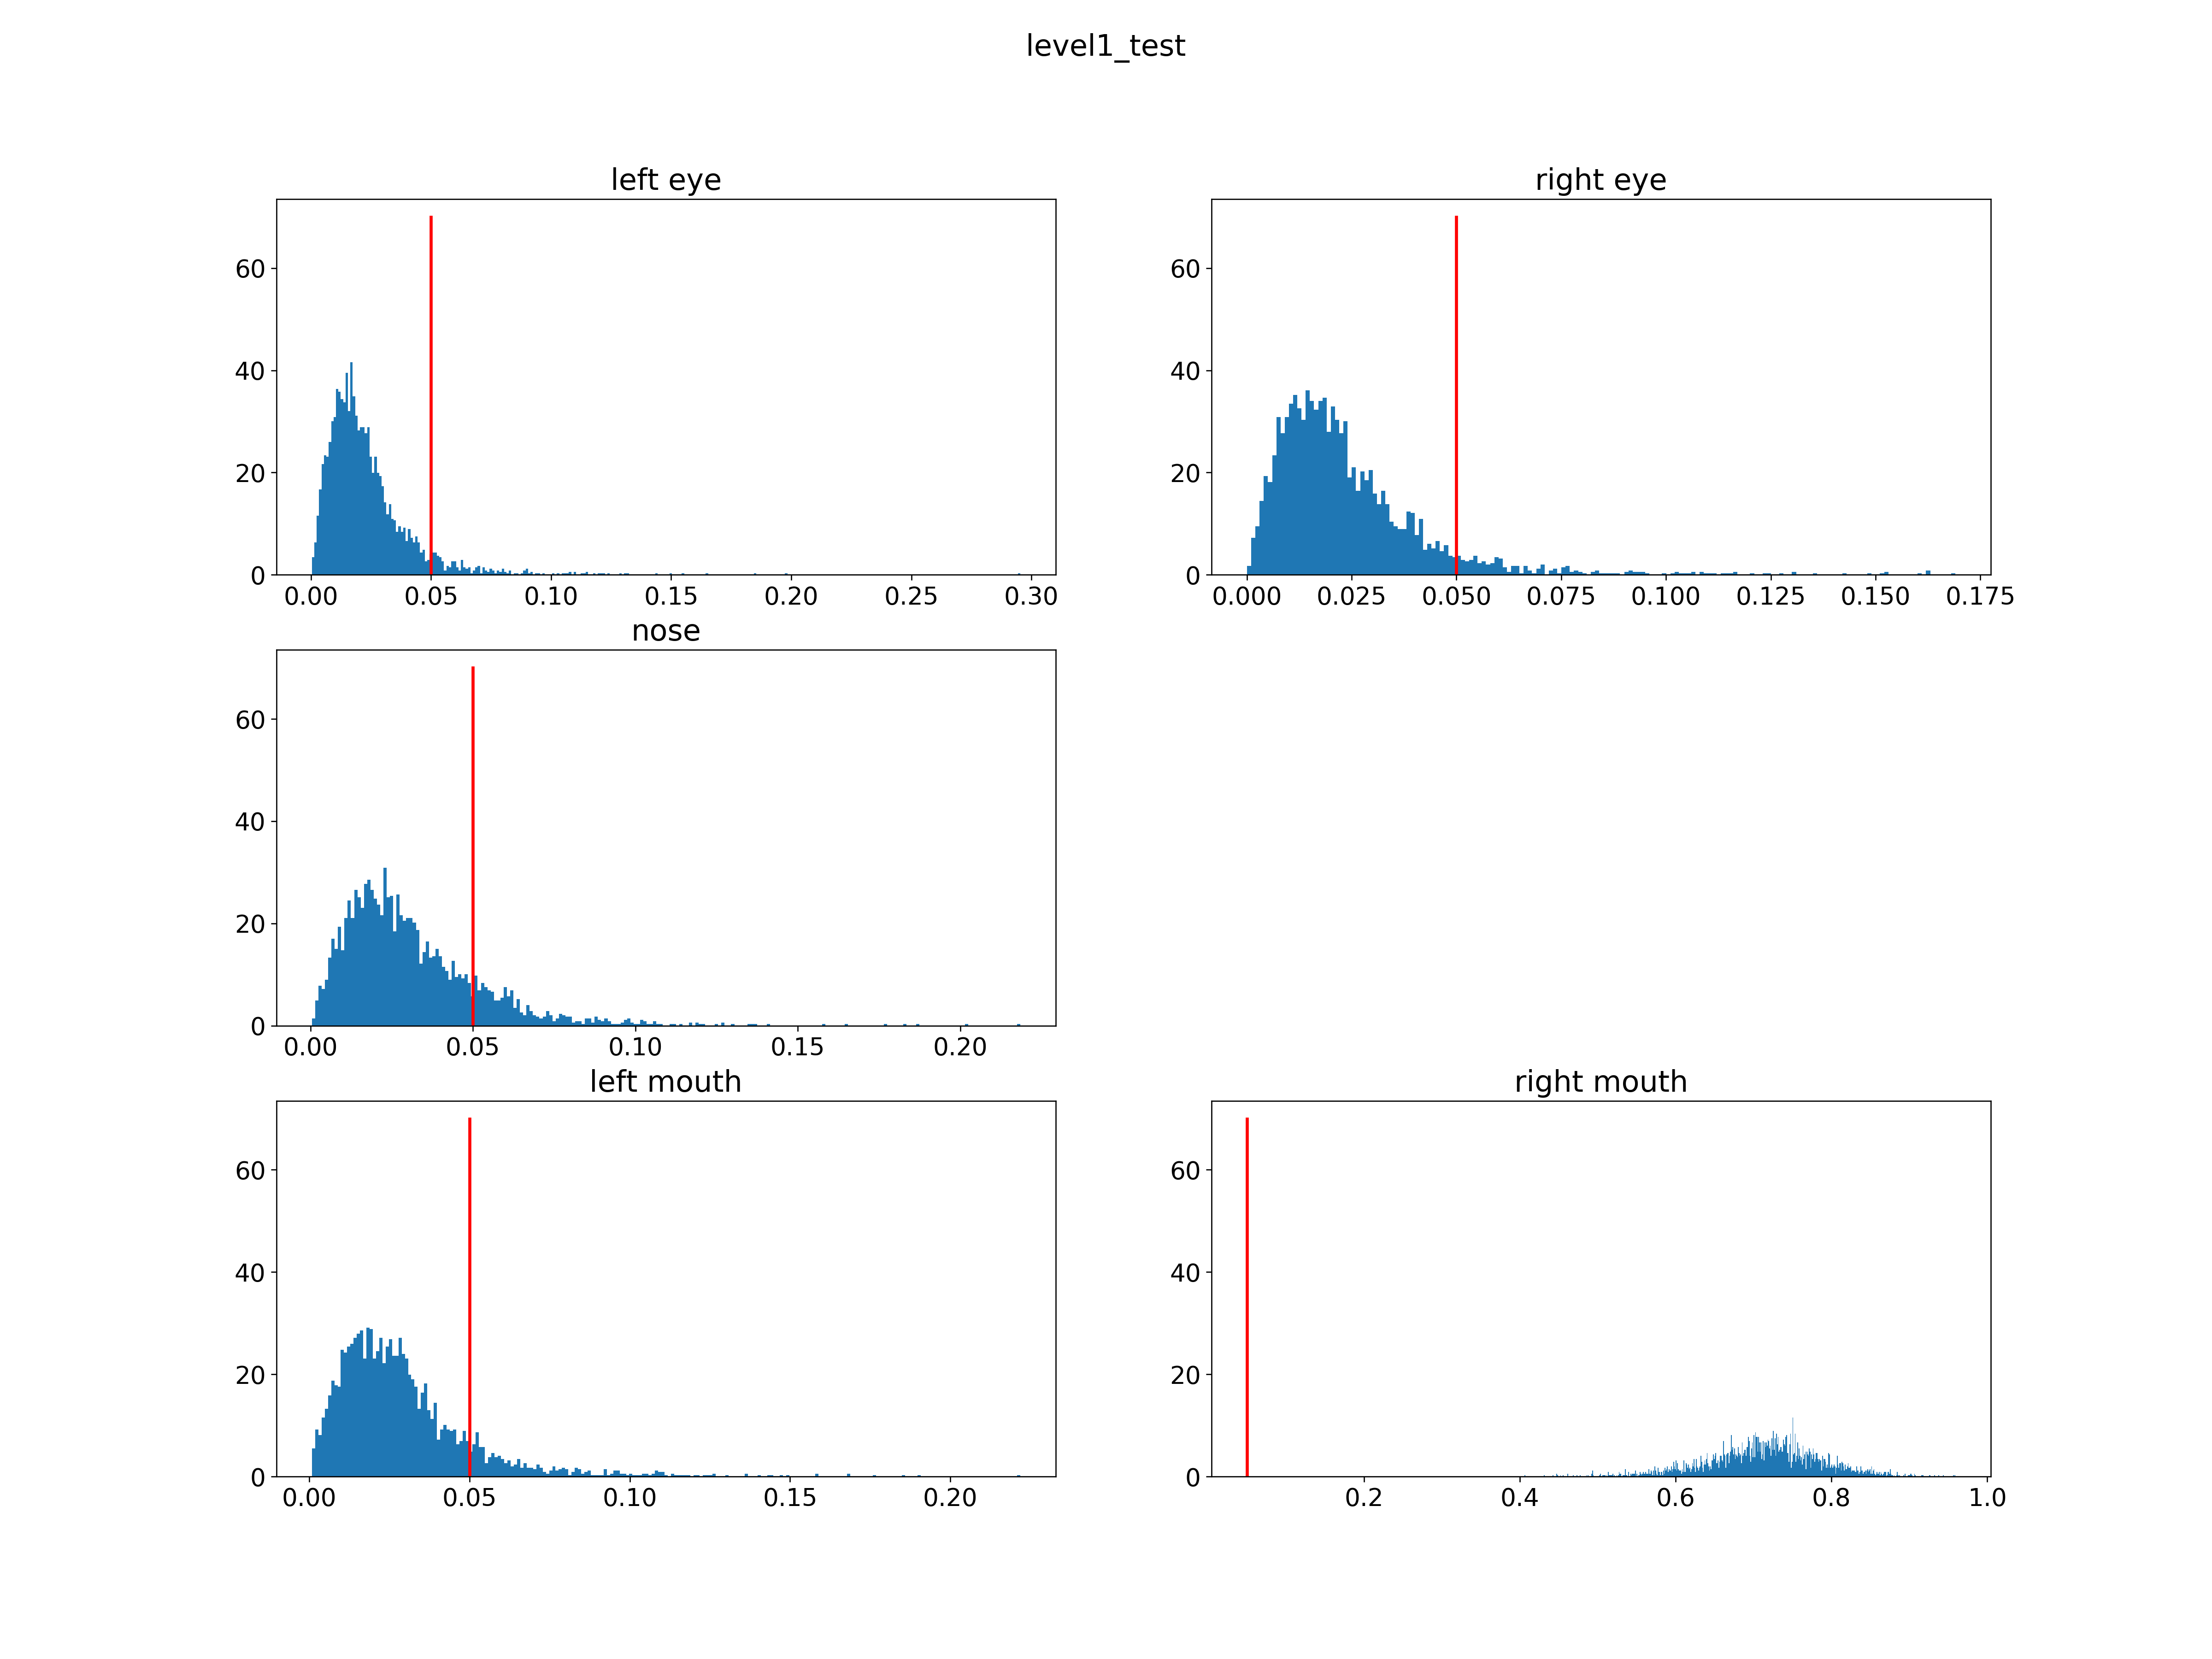
\includegraphics[scale=0.3]{images/level1_test}
	\caption{The error on each landmark in level 1}
	\label{1Fconv}
\end{figure}
\begin{figure}[h]
	\centering
	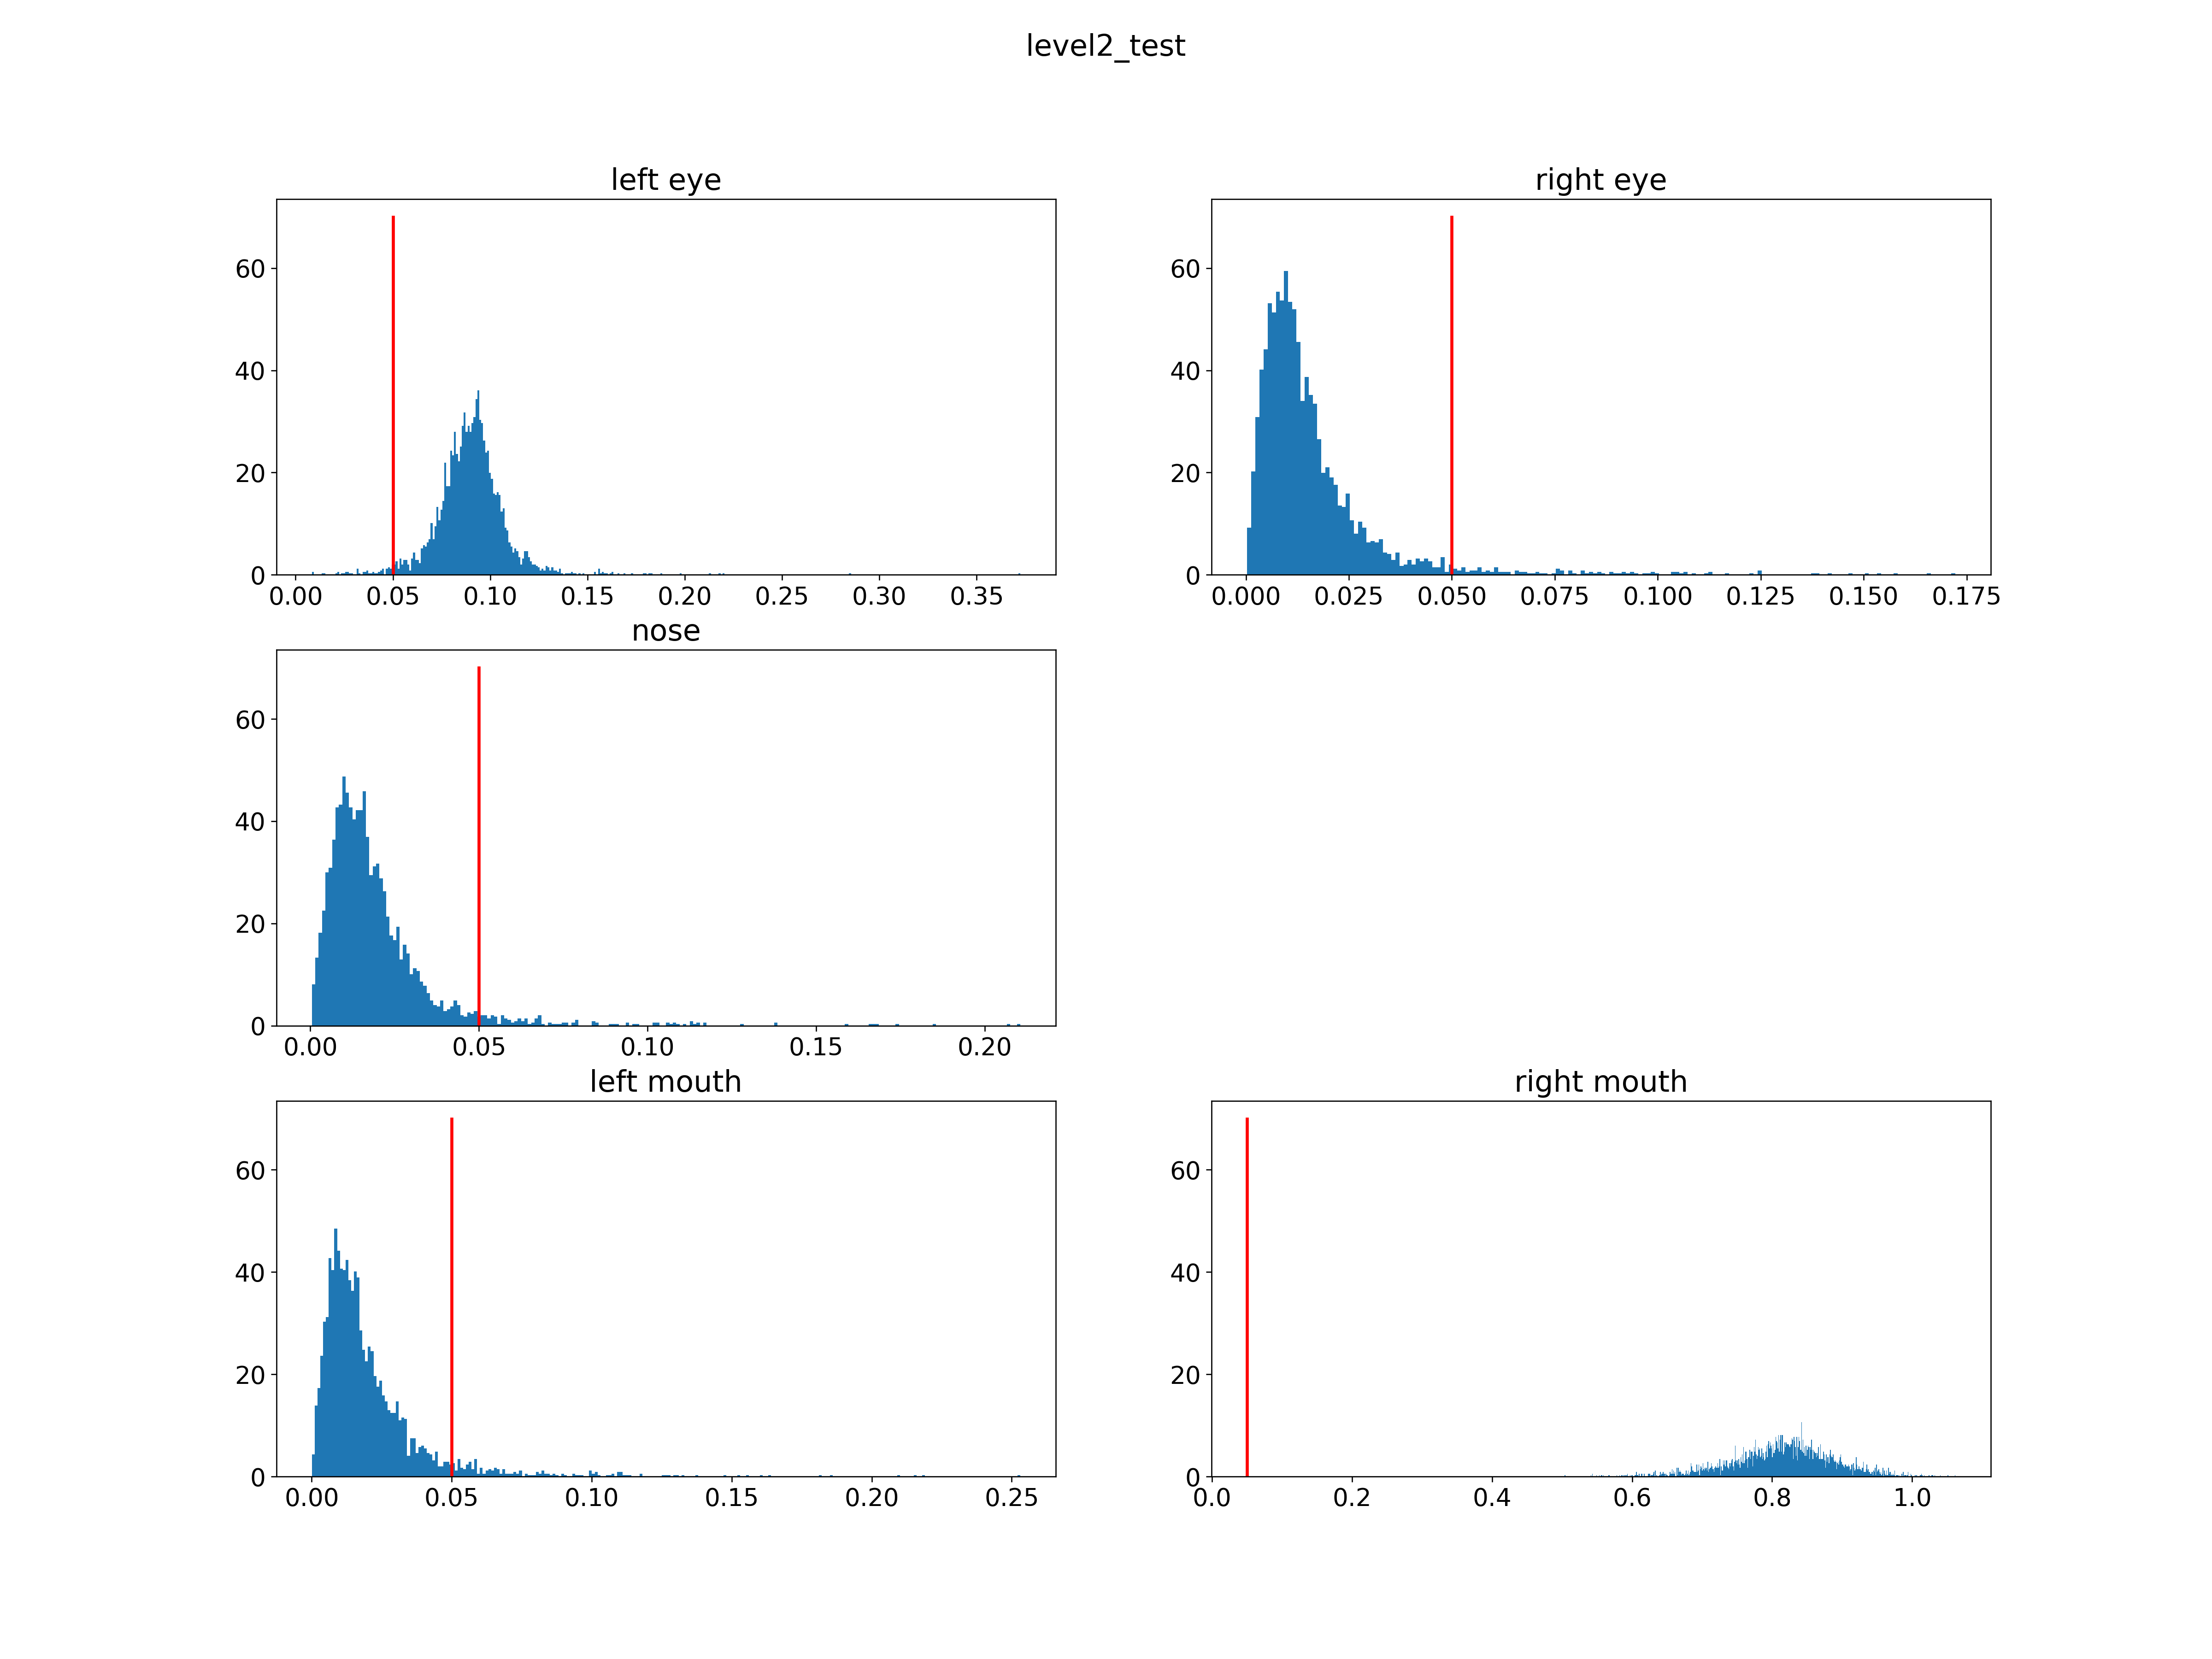
\includegraphics[scale=0.3]{images/level2_test}
	\caption{The error on each landmark in level 2}
	\label{1Fconv}
\end{figure}
\begin{figure}[h]
	\centering
	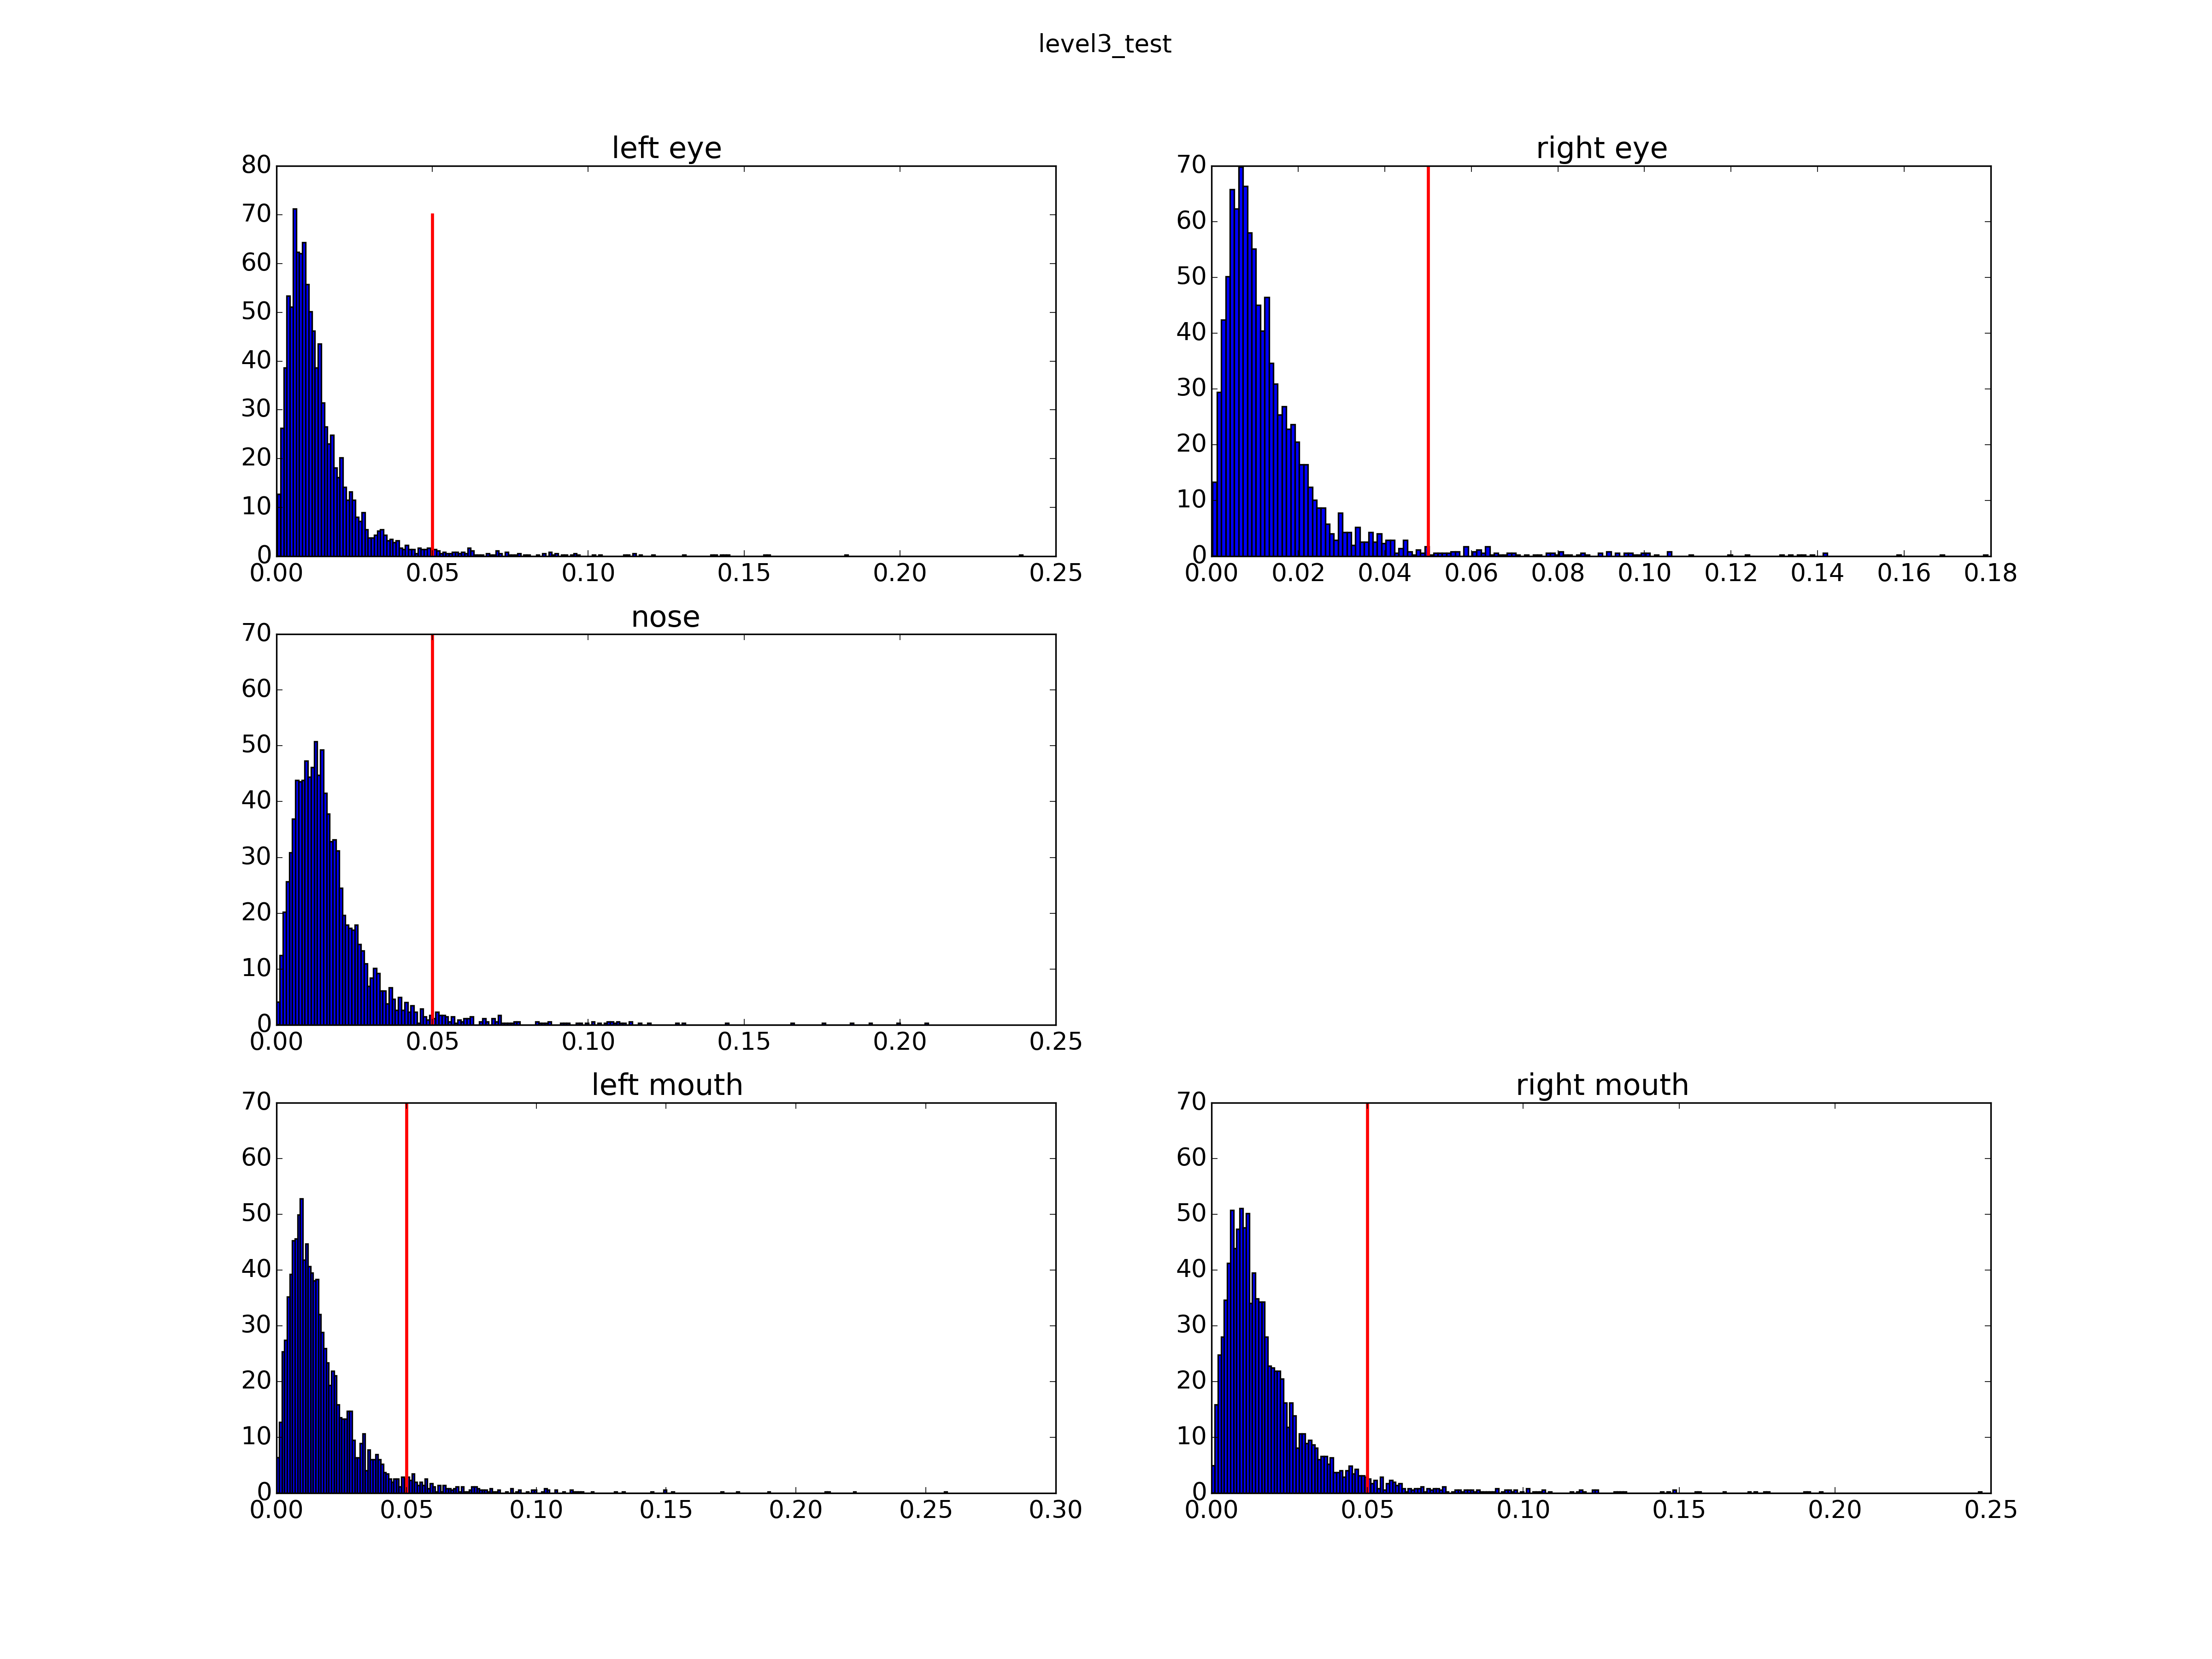
\includegraphics[scale=0.3]{images/level3_test}
	\caption{The error on each landmark in level 3}
	\label{1Fconv}
\end{figure}
According the charts, all the facial points are detected with high accuracy at all levels (except right mouth in level 1,2).
\subsection{Model with pronotum landmarks data}
The networks in the first level is modified to suitable with the prediction of landmarks on pronotum. For each pronotum, eight manual landmarks have been set. The bounding box is created depending on the coordinate of the manual landmark. The networks in the first level are used as followed:
\begin{itemize}
	\item F1 network recognizes whole pronotum bounding box with eight landmarks.
	\item EN1 network predicts the location of the first five-landmarks.
	\item NM1 network is used to estimated the position of last four-landmarks.
	\item At the end, the position of each landmark is average of the predicted position in the networks.
\end{itemize} 
\subsubsection{Data and training}
The dataset includes 293 pronotum images. The images are divided into three subset: training set (200 images), validation set (60 images) and test set (33 images). To enlarge the dataset during training, the image in training and validation set are augmentation by modifying the valued of red and green channel. So, at the end, we have 600 and 180 images in training and validation set, respectively.
\subsubsection{Testing}
The error rate of each network during training is shown in the table:\\
\begin{table}[h!]
	\centering
	\begin{tabular}{l r}
	Network & Loss \\ \hline
	F1 & 0.013 \\ \hline
	EN1 & 0.47\\ \hline
	NM1 &  0.5
	\end{tabular}
\end{table}\\
The model is tested on four images. The position of the landmark is located.
\begin{figure}[h!]
\centering
\subfloat[Test 1]{\label{}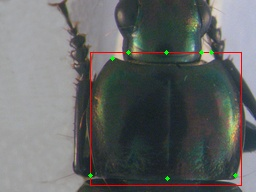
\includegraphics[width=0.45\textwidth]{./images/test1}}~~
\subfloat[Test 2]{\label{}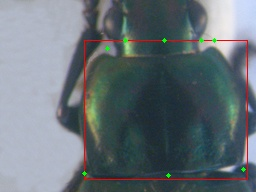
\includegraphics[width=0.45\textwidth]{./images/test2}}\\
\subfloat[Test 3]{\label{}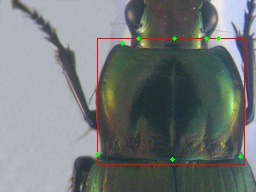
\includegraphics[width=0.45\textwidth]{./images/test3}}~~
\subfloat[Test 4]{\label{}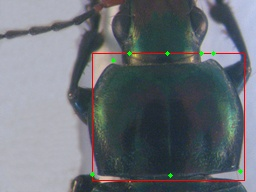
\includegraphics[width=0.45\textwidth]{./images/test4}}\\
\caption{The pronotum with predicted landmarks at level 1}
\label{figcentroidSize}
\end{figure}

Next: continue with the network of level 2, 3.
\section{Automatic ear detection with CNN}
Celia Cintas et al \cite{•} proposed a method based on Geometric Morphometric and Deep Learning for automatic ear detection and feature extraction in the form of landmarks. The convolutional neural network was trained with a set of manually landmarks examples. The network is able to provide the morphometric landmarks on ear image automatically.
\subsection{Dataset}
The image and manual landmark belong to the CANDELA initiative \cite{•}, a project includes geneticists, bioinformatics and social-anthropologists interested on Latin American. CANDELA contains 7500 images with the size of $2136 \times 3216$. The provided dataset contains 2753 images which extracted from the CANDELA dataset. For each image, a set of 45 landmarks and semi-landmarks provided by human operators. The dataset was split into a training set with 2051 images (75\%) and a validation set of 684 images (25\%).
\subsection{Network}
Three models were designed and trained for performing the automatic landmarks task.  These architectures are different in the number of convolution layers, the filter sizes, and the learning rate. An image with a single channel of the size  $96 \times 96$ with brightness scaled to [0,1], is taken as the input of the network. Fig.\ref{1Econv} shows the best architecture. In this architecture, a structure of two convolutional layers with the filters, followed by maximum pooling and dropout layer. This structure is repeated three times to obtain features at different levels with different size of filters. After extraction the features, two fully connected linear layers with 1500 units each and a dropout layer is hired. The output layer contains 90 output units (corresponding with 45 landmarks) for the predicted position of the landmarks. The implementation used Python and the Lasagne library \cite{}
\begin{figure}[h!]
	\centering
	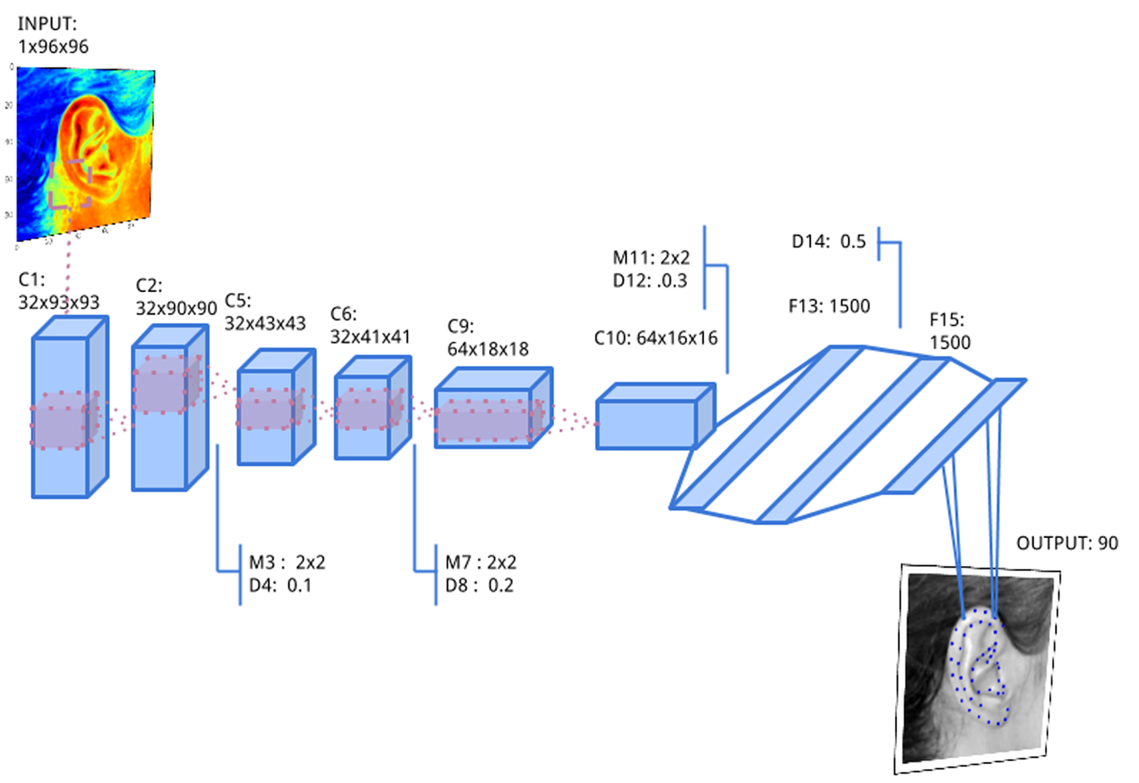
\includegraphics[scale=0.27]{images/ear_cnn}
	\caption{The best architecture for automatic ear's landmarks detection}
	\label{1Econv}
\end{figure}
\subsection{Experiments}
Following the article, the method is evaluated the usual quality metrics for regression problems, in particular $r^2$, root mean square error (RMSE), explained variance (EV), and Pearson's correlation. The accuracy of three architectures are shown in Table \ref{tbear1}. Also, in Table \ref{tbear2}, the RMSE for each landmarks is shown. The regression metrics were computed using \textit{scikit-learn}\cite{}.
\begin{table}[h!]
	\centering
	\begin{tabular}{l c c c}
	& Arch0 & Arch1 & Arch2 \\ \hline
	$r^2$ & 0.709 & 0.678 & 0.698 \\ \hline
	RMSE & 2.296 & 2.415 & 2.338\\ \hline
	EV & 0.976 & 0.974 &  0.975 \\ \hline
	Pearson & 0.988 & 0.987 &  0.988 \\ \hline	
	\end{tabular}
	\caption{Performance of three different ConvNet architectures}
	\label{tbear1}
\end{table}\\
\begin{table}[h!]
	\centering
	\begin{tabular}{l r}
	\# Landmark & RMSE \\ \hline
	1 & 1.8183 \\ \hline
	2 & 1.2216\\ \hline
	3 &  1.08651\\ \hline
	4 &  1.3291\\ \hline
	5 &  2.4477\\ \hline
	6 &  2.59746\\ \hline
	7 &  1.17571\\ \hline
	\end{tabular}
	\caption{RMS error for each landmark}
	\label{tbear2}
\end{table}\\
Because the CANDELA dataset is not open. Another dataset was chosen to study the network. The new dataset was used for the Facial Keypoint Detection including 7049 gray-scale images ($96 \times 96$). For each image, we are supported learn to find the position of 15 landmarks. After dropping some missing data, the dataset remains 2140 images. All the images with coordinates of manual landmarks is stored in csv file and fetched into the network. The training and validation loss are shown in Fig. \ref{}.
\begin{figure}[h!]
	\centering
	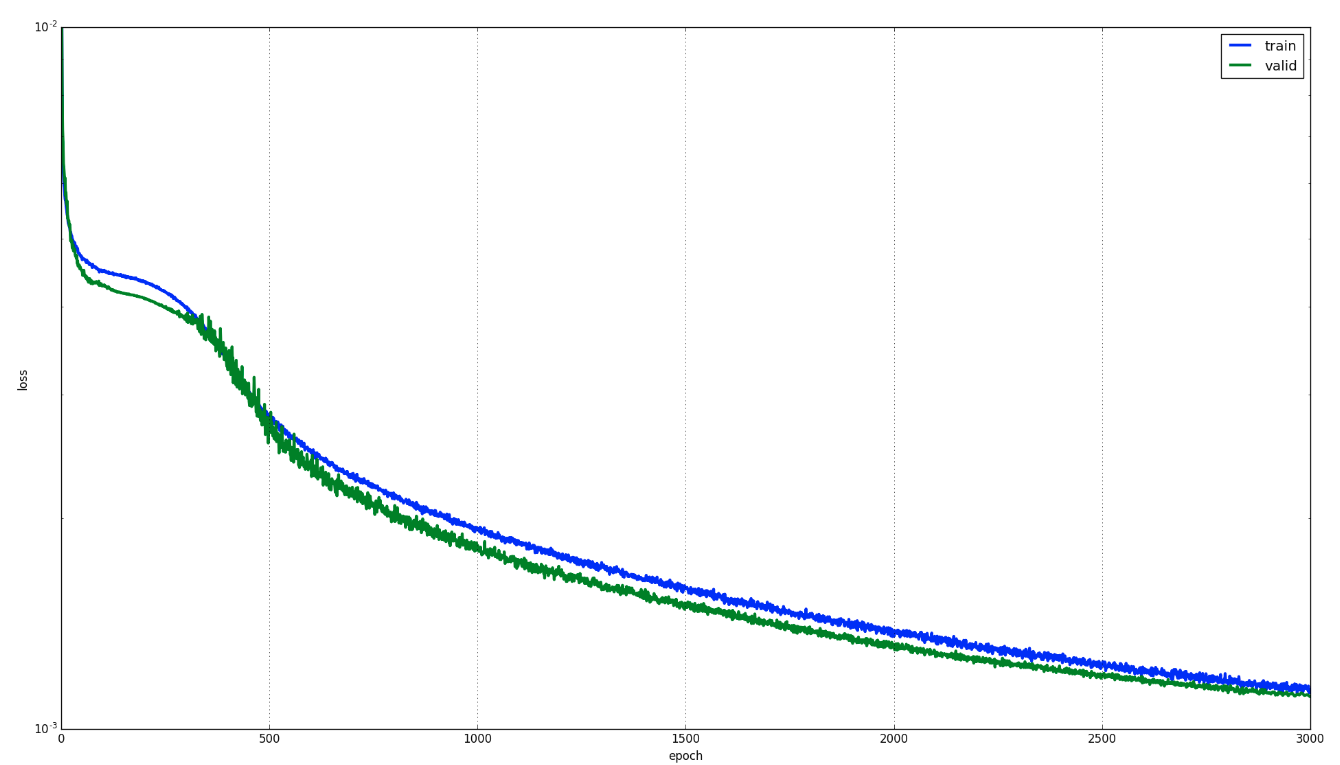
\includegraphics[scale=0.27]{images/trainloss}
	\caption{The loss of Ear-CNN network with facial point dataset}
	\label{1Econv}
\end{figure}
	\chapter{Convolutional Neural Network for predicting morphometry landmarks}
In the previous chapter, we have studied two CNNs \cite{sun2013deep, cintas2016automatic} that applied to predict the keypoints on human face and human ear. Then, we have applied their methods to detect the landmarks (keypoints) on thorax of beetle but the obtained results are not really impressed. In this chapter, based on the knowledge of Deep Learning and CNN, we propose a new archtecture to predict the landmarks on some parts of beetle. We also describe the process that we have used to augment the dataset for training and evaluating the model.

\section{Network architecture designing}
In the process, we have tried three networks models before obtaining the final architecture for detecting the landmarks on beetle images. Like other CNN models, we have employed the classical layers to construct the models, i.e, convolutional layer, maximum pooling layers and full-connected layer.

The first architecture is very classical one, it receives an image with the size of $1 \times 192 \times 256$ as the input. Then, the network consists on three repeated strucutre of a convolutional layers followed by a maximum pooling layers. Most CNNs, the hyperparameters of convolutional layers have been set to increase the depth of the images from the first layer to the last layer. That is reflected in the setting of the number of filters at each convolutional layer. So, the depths of convolutional layers increase from $32, 64, $ and $128$ with different size of the kernels: $3 \times 3$, $2 \times 2$ and $2 \times 2$, respectively. Inserting pooling layers after a convolutional layers is a common periodcally. The pooling layer effects to progressively reduce the spatial size of the representation to reduce the number of parameters, computation in the network, and it also controls over-fitting. The operations of pooling layers independent on every depth slice of the input. The most common form is a pooling layer with filters of size $(2 \times 2)$ and a stride of $2$. It downsamples every depth by $2$ along width and height of the input. Thefore, all the kernels of maximum pooling layers have the same size of $2 \times 2$ with a stride of $2$ as usual. At the end of the model, three full-connected layers have been added to extract the global relationship between the features and to procedure the outputs. The first of two full-connected layers are set to non-linearity to make sure these nodes interact well and take into account all possible dependencies at the feature level. The outputs of the full-connected layers are $500, 500$ and $16$. The output of the last full-connected layer corresponds to the coordinates ($x$ and $y$) of $8$ landmarks which we would like to predict. Fig. \ref{fignet1} shows details of the first model: The orange rectangles represent for convolutional layers while the yellow rectangles represent for maximum pooling layers and three full-connected layers with their parameters are presented at the end of the model.

\begin{figure}[!h]
	\centering
	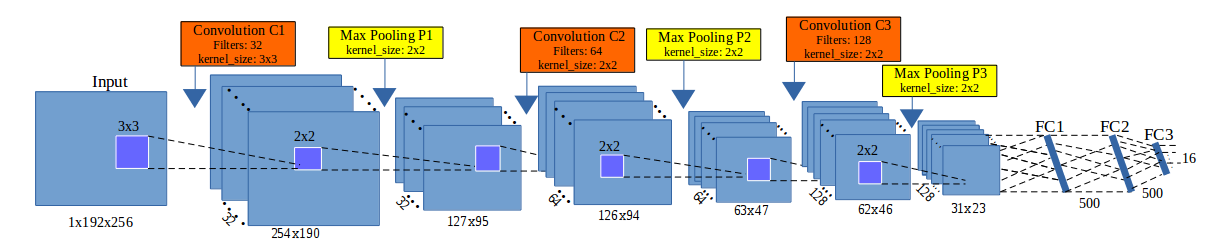
\includegraphics[scale=0.4]{images/net1}
	\caption{The architecture of the first model}
	\label{fignet1}
\end{figure}

The second architecture is modified from the first model. The layers are kept the same as the first one but the outputs of the first of two full-connected layers are changed from $500$ (in the first model) to $1000$ (Fig. \ref{}). Increasing the value at full-connected layers is hoping to obtain more features from convolutional layer and to prevent the over-fitting. 

\begin{figure}[h]
	\centering
	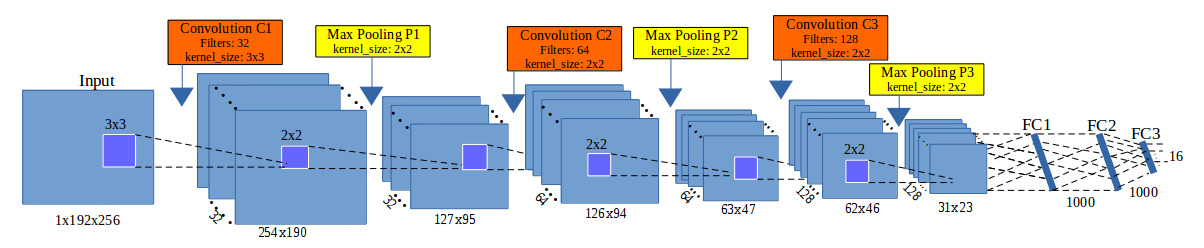
\includegraphics[scale=0.4]{images/net2}
	\caption{The architecture of the second model}
	\label{fignet2}
\end{figure}

To build the third architecture, we have used the definition of \textit{elementary block}. An {elementary block} is defined as a sequence of convolution ($C_{i}$), maximum pooling ($P_i$) and dropout ($D_i$) layers. This significantly reduces overfitting and gives major improvements over other regularization methods \cite{}. The idea of dropout is to include some variations between different runs. During training phase, dropout samples are done from an exponential number of different ``thinned” network. At test phase, it is easy to approximate the effect of averaging the prediction of all thinned networks by simply using a single unthinned network with smaller weights. So, we have modified the architecture by combining some \textit{elementary blocks}. Fig. \ref{fignet3} illustrates the layers in the third architecture. For our purpose, we have assembled \textbf{3 elementary blocks}. The parameters for each layer in each elementary block are as below, the list of values follows the order of elementary blocks ($i = [1..3]$):
\begin{itemize}
	\item CONV layers:
	\begin{itemize}
		\item Number of filters: $32, 64, $ and $128$
		\item Kernel filter sizes: $(3 \times 3), (2 \times 2), $ and $(2 \times 2)$
		\item Stride values: $1, 1, $ and $1$
		\item No padding is used for CONV layers 
	\end{itemize}
	\item POOL layers:
		\begin{itemize}
			\item Kernel filter sizes: $(2 \times 2), (2 \times 2), $ and $(2 \times 2)$
			\item Stride values: $2, 2, $ and $2$
			\item No padding is used for POOL layers
		\end{itemize}
	\item DROP layers:
		\begin{itemize}
			\item Probabilites: $0.1, 0.2, $ and $0.3$
		\end{itemize}
\end{itemize}

Three full-connected layers (FC) are kept the same as the second architecture: FC1 and FC2 have $1000$ outputs, the last full-connected layer (FC3) has $16$ outputs. As usual, a dropout layer is inserted between FC1 and FC2 with a probability equal to $0.5$.
\begin{figure}[h]
	\centering
	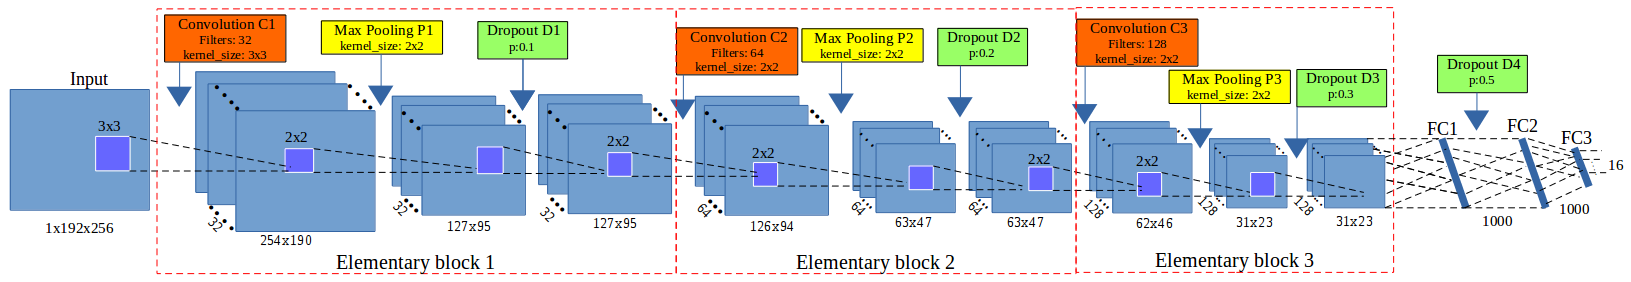
\includegraphics[scale=0.3]{images/arch_model}
	\caption{The architecture of the third model}
	\label{fignet3}
\end{figure}

The core of neural network is training over iteration. There are many ways to optimize the learning algorithm, but gradient descent \cite{} is currently a good choice to establish the way of optimizing the loss in neural network. The core idea is following the gradient until we statify with the results will remain the same. So, we have chosen gradient descent in the backward phase to update the values of learnable parameters and to increase the accuracy of the network. The networks are designed with a small sharing learning rate and a momentum. The learning rate is initialized at $0.03$ and stopped at $0.00001$, while the momentum is updated from $0.9$ to $0.9999$. Their values are updated over training time to fit with the number of epochs \footnote{An epoch is a single pass through the full training set}. The implementation of the architectures have been done on Lasagne framework \cite{} by Python. 

\section{Data augmentation}
A characteristic of machine learning and deep learning is using a volume dataset to train the model. Of course, in practice, we are not always have enough data for training. One way to solve this problem is to create the fake data from real data and to add it to the training set. Dataset augmentation has been a particularly effective technique for a specific problem. For example, in images classification problem, the operations like translating,  rotating or scaling the images have also effective. The fake images may be generated by translating (rotating or scaling) in each direction. Besides, injecting noise in the input can also see as a form of data augmentation.

Our dataset includes $293$ images of beetles (for each anatomical part). All the images are taken with the same camera in the same condition with a resolution of $3264 \times 2448$. Each image has a set of manual landmarks provided by biologists, i.e, each thorax has $8$ landmarks, each head has $10$ landmarks. Applying CNNs to train each part with a small number of images to reach good results is impossible. So, we need to augment the dataset before training the networks. Firstly, we have found that the original solution of the images $(3264 \times 2448)$ are heavy for the neural network. For performance considerations, in most of CNNs \cite{}, the size of the input is limited to $256 \times 256$ pixels, so we have decided to down-sampling the images to a new resolution $(256 \times 192)$ (to respect the ratio between $x$ and $y$). Of course, the coordinates of manual landmarks have been also scaled to fit with the new resolution of the images. In usual way, the transformations have been used to augment the dataset (i.e rotation, translation,\ldots) but the analysis of image by CNN is most often translation and rotation invariant. Therefore, two other procedures have been imaged to increase the number of images in the dataset $(256 \times 192)$.

The first procedure is to change the value of a color channel in the original image to generate a new image. According to that, a constant is added to one of the RGB channels each time it is used for training. Each constant is sampled in a uniform distribution $\in [1, N]$ to obtain a new value caped at $255$. For example, Fig. \ref{figaug1} shows an example when we added a constant $c = 10$ to each channel of an original image. Following this way, we can generate three version from an image.
\begin{figure}[h]
	\centering
	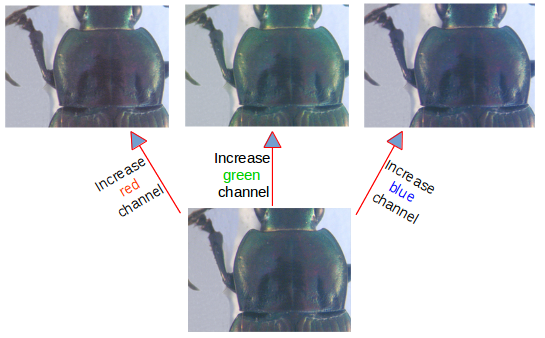
\includegraphics[scale=0.5]{images/inc_channels}
	\caption{A constant $c = 10$ has been added to each channel of an original image}
	\label{figaug1}
\end{figure}

In the second procedure, we have applied the opposite procedure to the first one. Instead of adding the value, we separate the channels of RGN into three gray-scale images as the network works on single channel images. At the end of the processes, we are able generate six versions from an original image. In total, we have $293 \times 7 = 2051$ images for each anatomical part of beetle (an original image and six generated images). However, we have not used all images for training and validation. So, we have chosen $260$ original images and their generations ($1820$ images) of each dataset for training and validation processes, the remaining images ($33$ original images) are used for test process.

\begin{figure}[h]
	\centering
	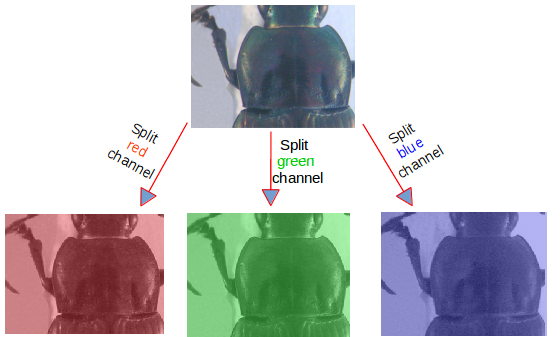
\includegraphics[scale=0.5]{images/sp_channels}
	\caption{Three channels (red, green, blue) are separated from original image}
	\label{figaug2}
\end{figure}

In practical, to obtain a fast convergence during the computing, it is useful to normalize the brightness of the images to $[0,1]$ instead of $[0, 255]$ and the coordinates of the landmarks have been also normalized. 
\section{Experiments and results}
Before widely applying to all anatomical parts, we have firstly tried with thorax part to evaluate the performance. The networks have been trained in $5, 000$ epochs on Ubuntu machine by using NVIDIA TITAN X cards. The set of images that used for training and validation are merged together. 

During the training, the images are chosen randomly from the dataset with a ratio of $60\%$ for training and $40\%$ for validation. The training step takes into account a pair of information (\textit{images, manual landmarks coordinates})  as training data. In the context of deep learning, landmark prediction can be seen as a regression problem. So, we have used Root Mean Square Error (RMSE) to compute the loss of implemented architectures.

At the test phase, images without landmarks are given to the trained network to produce output coordinates of the predicted landmarks. The results then evaluated by comparing with the manual landmarks coordinates provided by biologists which have been seen as ground truth. Fig. \ref{figloss1} shows the training errors and the validation errors during traning phase of the first architecture. The blue curve presents the RMSE errors of training process, the green curve presents the validation errors. Clearly, over-fitting has appeared in the first model. The training losses are able to decrease but the validation losses are stable. In the second model (section \ref{}), we have modified the parameters of full-connected layers to prevent the over-fitting but it seems that this solution is still not suitable. The over-fitting is also appeared as the first model.

\begin{figure}[h]
	\centering
	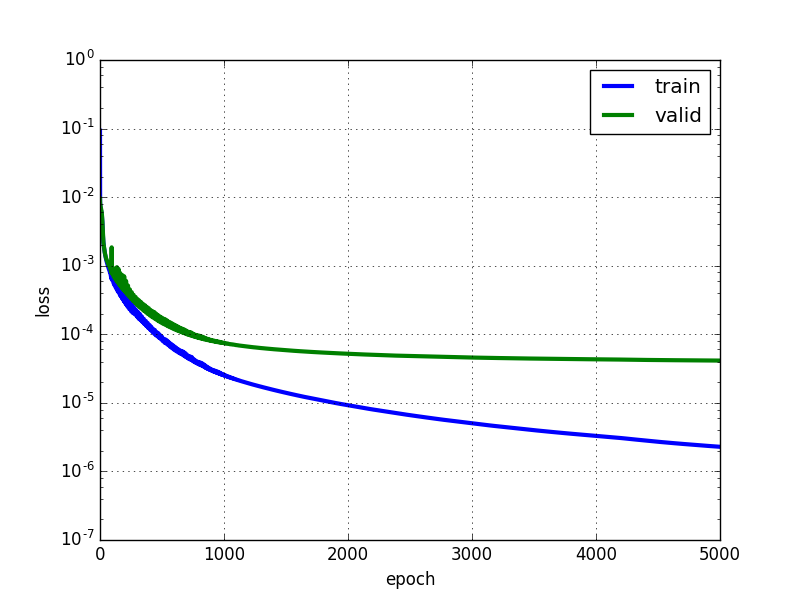
\includegraphics[scale=0.6]{images/cnnmodel3_5000_pronotum_v13_without_dropout_normalized_data_loss}
	\caption{The training and validation losses of the first model}
	\label{figloss1}
\end{figure}

Then, we have continued to train the third model on the same dataset of thorax images. Fig. \ref{figloss2} illustrates the losses during the training of the third model. Like the previous figure (Fig. \ref{figloss1}), the blue line is training losses, the green line is validation losses. In the opposite with two previous models, the losses are different (far) from the beginning but after several epochs, the values become more proximate and the over-fitting problem has been solved. This proves that adding dropout layers to build the elementary blocks have been effects to prevent over-fitting and contributory improve the accuracy of the model. \textit{So, we have decided to keep the architecture of the third model for our landmarking problem.}

\begin{figure}[h]
	\centering
	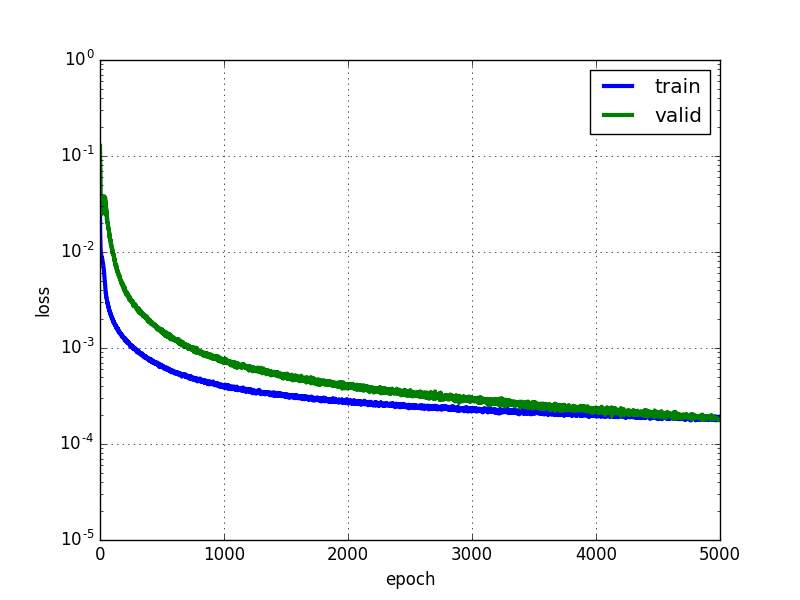
\includegraphics[scale=0.6]{images/loss_v16}
	\caption{The training and validation losses of the third model}
	\label{figloss2}
\end{figure}

In order to have the predicted landmarks for all thorax images (instead of only $33$ images), we have applied \textit{cross-validation} to choose the test images, called \textit{round}. For each time, we have chosen a different fold of $33$ images as testing images, the remaining images are used as training and validation images ($293/33 \approx 9$ rounds). Following that, the network will be trained with many different datasets, then the trained model will be used to predicted the lanmarks on the images in the corresponding test set. Table. \ref{tbltrainingloss} resumes the losses of $9$ rounds when we trained the third model on thorax images.

\begin{table}[h!]
	\centering
	\begin{tabular}{l l l}
	Round & Training loss & Validation loss \\ \hline
	1 & 0.00018 & 0.00019  \\ \hline
	2 & 0.00019 & 0.00021 \\ \hline
	3 & 0.00019 & 0.00026 \\ \hline
	4 & 0.00021 & 0.00029 \\ \hline
	5 & 0.00021 & 0.00029 \\ \hline
	6 & 0.00019 & 0.00018 \\ \hline
	7 & 0.00018 & 0.00018 \\ \hline
	8 & 0.00018 & 0.00021 \\ \hline
	9 & 0.00020 & 0.00027 \\ \hline
	\end{tabular}
	\caption{\small{The losses during training the third model on thorax images}}
	\label{tbltrainingloss}
\end{table}

To evaluate the coordinates of predicted landmarks, the correlation metrics have been computed the correlation between the manual landmarks and their corresponding predicted one. Table. \ref{tblcorrelation} shows the correlation scores of $3$ metrics (using \textit{scikit-learn} \cite{}), i.e, coefficient of determination ($r^2$), explained variance (EV), and Pearson correlation. All of three metrics have the same possibility. The best score is $1.0$ if the correlation data is good, lower values are worse. It means that our predicted coordinates are very close with the ground truth. However, the measure is not enough good to provide a useful result to biologists. Moreover standing on the side of image processing, we are looking forward to  seeing the predicted coordinates than the statistical results.

\begin{table}[htbp]
	\centering
	\begin{tabular}{|c|p{2cm}|p{2cm}|p{2cm}|}
		Metric & $\mathbf{r^{2}}$ & \textbf{EV} & \textbf{Pearson} \\ \hline
		Score & $\textbf{0.9952}$ & $\textbf{0.9951}$ & $\textbf{0.9974}$ 
	\end{tabular}
	\caption{Correlation scores between manual landmarks and predicted landmarks}
	\label{tblcorrelation}
\end{table}

The main goal of computing is to predict the coordinates of landmarks, so the distances (in pixels) between the coordinates of manual landmarks and corresponding predicted landmarks have been taken into account on all images. Then, the average of distances are computed by landmarks. Table. \ref{} shows the average distances by landmarks on all images of thorax dataset. With images of resolution $256 \times 192$, we can
consider that an error of $1\%$ corresponds to $2$ pixels that could
be an acceptable error. Unhappily, our results exhibit average
distance of $4$ pixels in the best case, landmark $1$ and more than
$5$ pixels, landmark $6$. Other error distances are more than $2\%$
pixels.

\begin{table}[htbp]
	\centering
	\begin{tabular}{|c|c|}
		\hline
		\textbf{Landmark} & \textbf{Distance} (in pixels) \\ \hline
		1 & 4.002  \\ \hline
		2 & 4.4831 \\ \hline
		3 & 4.2959 \\ \hline
		4 & 4.3865 \\ \hline
		5 & 4.2925 \\ \hline
		6 & 5.3631 \\ \hline
		7 & 4.636 \\ \hline
		8 & 4.9363 \\ \hline
	\end{tabular}
	\caption{The average distances on all images per landmark.}
\end{table}

Fig. \ref{figchartlm1} shows the distribution of the distances on the first landmark of all images. The accuracy based on the distance in each image can be
separated into three spaces: the images have the distance less
than average value ($4$ pixels): $56.66\%$; the images have the
distance from average value to $10$ pixels (average distance plus
standard deviation): $40.27\%$; and the images have the distance
greater than $10$ pixels: $3.07\%$.

\begin{figure}[htbp]
	\centerline{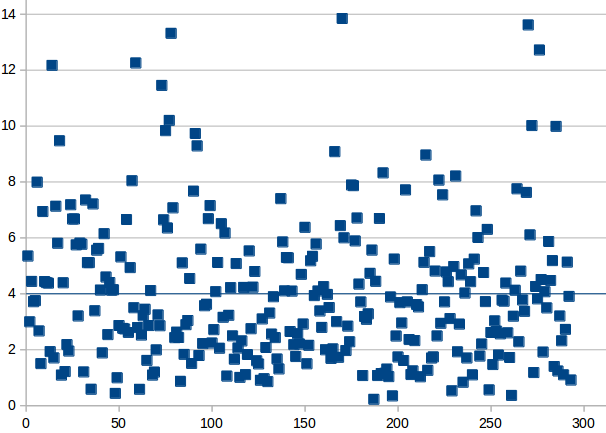
\includegraphics[scale=0.5]{images/statistic_pronotum_from_scratch_lm1}}
	\caption{The distribution of the distances on the first landmark. The blue line is the average value of all distances.}
	\label{figchartlm1}
\end{figure}

To illustrate this purpose, Fig. \ref{figrsexample} shows the predicted landmarks on two test images. One can note that even some predicted landmarks (Fig. \ref{figsub1}) are closed to the manual ones, in some case (Fig. \ref{figsub2}) the predicted ones are far from the expect results. The next step has been dedicated to the improvement of these results.

\begin{figure}[htbp]
    \centering
    \subfloat[Image with well-predicted landmarks]{\label{figsub1}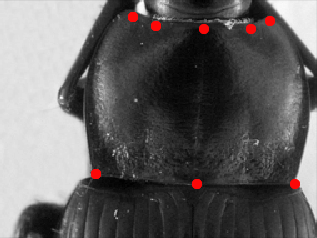
\includegraphics[width=0.35\textwidth]{images/fn_accuracy}}~~
\subfloat[Image with inaccuracy landmarks]{\label{figsub2}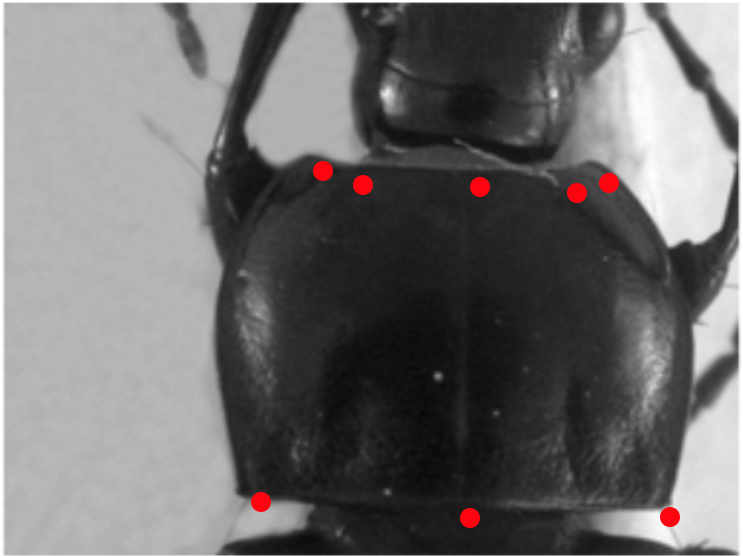
\includegraphics[width=0.35\textwidth]{images/plandmark2}}\\    
    \caption{The predicted landmarks, in red,  on the images in test set.}
    \label{figrsexample}
\end{figure}

From the success of the third architecture on thorax dataset, we apply the same procedures (data augmentation, training, \ldots) on other parts of beetle: \textit{elytra and head}. However, we have modified the number of the last full-connected layer to adapt with each dataset before training. Arcoding, the values at the last full-connected layer are set to $22$ and $20$ outputs corresponds to $11$ and $10$ landmarks on elytra and head, respectively. Of course, we have also applied \textit{cross-validation} to select testing data to get all predicted landmarks for all images in each dataset. Then, the quality of predicted landmarks are evaluated by comparing with the corresponding manual landmarks (distance computation). Table .\ref{tblavgdiselytra} and \ref{tblavgdishead} show the average distances on each landmark of elytra and head anatomical, respectively.

\begin{table}[htbp]
\begin{minipage}{0.5\linewidth}
	\centering
	\begin{tabular}{|c|c|}
		\hline
		\textbf{Landmark} & \textbf{Distance} (in pixels) \\ \hline
		1 & 3.8669  \\ \hline
		2 & 3.9730 \\ \hline
		3 & 3.9166 \\ \hline
		4 & 3.8673 \\ \hline
		5 & 4.0151 \\ \hline
		6 & 4.8426 \\ \hline
		7 & 5.2125 \\ \hline
		8 & 5.4685 \\ \hline
		9 & 5.2692 \\ \hline
		10 & 4.0709 \\ \hline
		11 & 3.9896 \\ \hline
	\end{tabular}
	\caption{\small{The average distance on all images per landmark on \textbf{elytra} images}}
	\label{tblavgdiselytra}
\end{minipage}
\hfill
\begin{minipage}{0.5\linewidth}
	\centering
	\begin{tabular}{|c|c|}
		\hline
		\textbf{Landmark} & \textbf{Distance} (in pixels) \\ \hline
		1 & 5.5280  \\ \hline
		2 & 5.1609 \\ \hline
		3 & 5.3827 \\ \hline
		4 & 5.0345 \\ \hline
		5 & 4.8393 \\ \hline
		6 & 4.4516 \\ \hline
		7 & 4.7937 \\ \hline
		8 & 4.5322 \\ \hline
		9 & 5.1412 \\ \hline
		10 & 5.0564 \\ \hline
	\end{tabular}
	\caption{\small{The average distance on all images per landmark on \textbf{head} images}}
	\label{tblavgdishead}
\end{minipage}
\end{table}




 Table. \ref{tbltraininglosselytra} and \ref{tbltraininglosshead} show the losses during training process  of the third model on elytra and head dataset, respectively.

\begin{table}[htbp]
\begin{minipage}{0.5\linewidth}
	\centering
	\begin{tabular}{l l l}
	Round & Training loss & Validation loss \\ \hline
	1 & 0.00019 & 0.00012  \\ \hline
	2 & 0.00020 & 0.00012 \\ \hline
	3 & 0.00019 & 0.00012 \\ \hline
	4 & 0.00020 & 0.00011 \\ \hline
	5 & 0.00018 & 0.00010 \\ \hline
	6 & 0.00019 & 0.00013 \\ \hline
	7 & 0.00018 & 0.00013 \\ \hline
	8 & 0.00018 & 0.00017 \\ \hline
	9 & 0.00019 & 0.00012 \\ \hline
	\end{tabular}
	\caption{\small{The losses during training the third model on \textbf{elytra} images}}
	\label{tbltraininglosselytra}
\end{minipage}
\hfill
\begin{minipage}{0.5\linewidth}
	\centering
	\begin{tabular}{l l l}
	Round & Training loss & Validation loss \\ \hline
	1 & 0.00023 & 0.00032  \\ \hline
	2 & 0.00027 & 0.00044 \\ \hline
	3 & 0.00026 & 0.00051 \\ \hline
	4 & 0.00026 & 0.00058 \\ \hline
	5 & 0.00027 & 0.00072 \\ \hline
	6 & 0.00025 & 0.00050 \\ \hline
	7 & 0.00023 & 0.00019 \\ \hline
	8 & 0.00024 & 0.00021 \\ \hline
	9 & 0.00025 & 0.00027 \\ \hline
	\end{tabular}
	\caption{\small{The losses during training the third model on \textbf{head} images}}
	\label{tbltraininglosshead}
\end{minipage}
\end{table}

Fig. \ref{figelytraloss} shows the loss curves of training and validation processes of two rounds on elytra part.

\begin{figure}[htbp]
    \centering
    \subfloat[The first fold]{\label{figel1}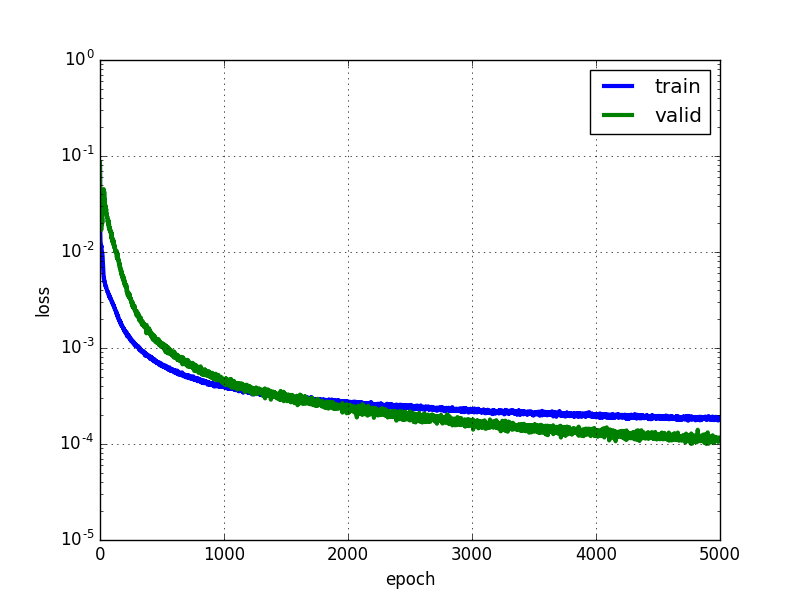
\includegraphics[width=0.45\textwidth]{images/cnnmodel3_5000_elytre_1000_output_v10_loss}}~~
\subfloat[The eight fold]{\label{figel2}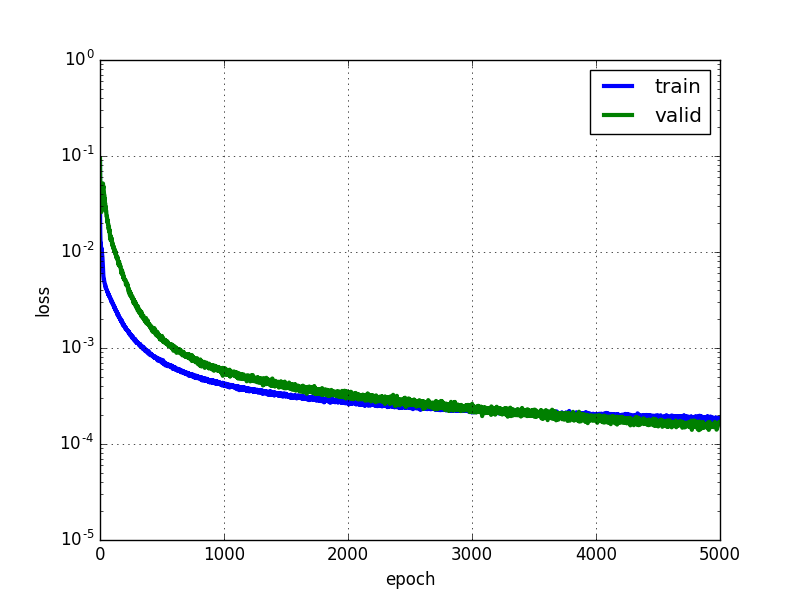
\includegraphics[width=0.45\textwidth]{images/cnnmodel3_5000_elytre_1000_output_v18_loss}}\\    
    \caption{The losses of two training examples on elytra part }
    \label{figelytraloss}
\end{figure}

\begin{figure}[htbp]
    \centering
    \subfloat[The first fold]{\label{figel1}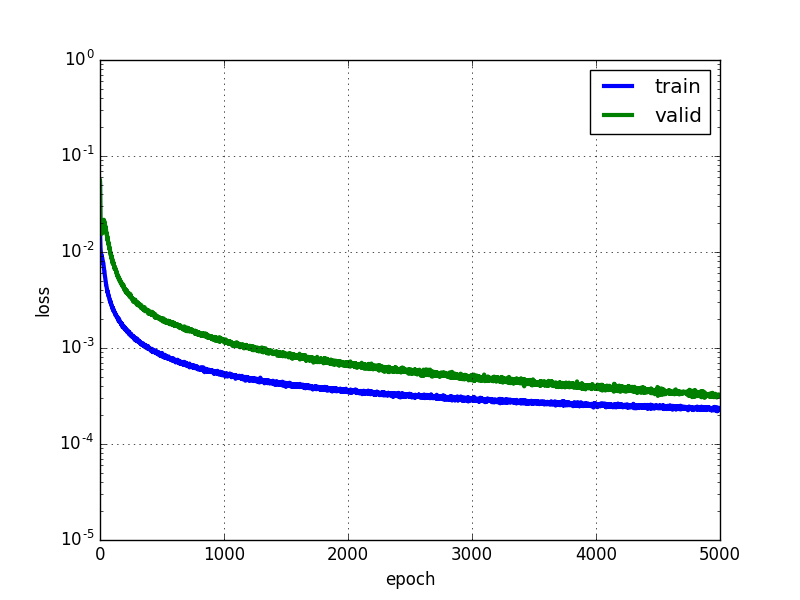
\includegraphics[width=0.45\textwidth]{images/cnnmodel3_5000_tete_1000_output_v10_loss}}~~
\subfloat[The eight fold]{\label{figel2}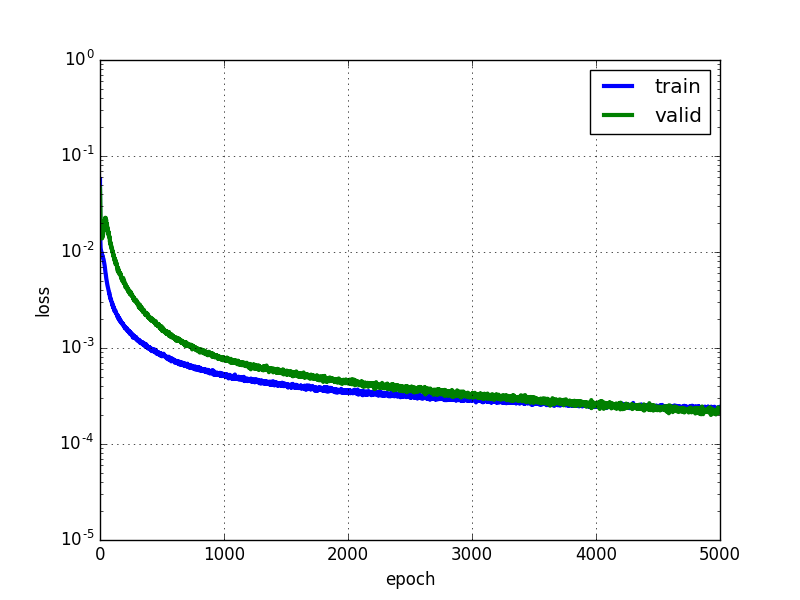
\includegraphics[width=0.45\textwidth]{images/cnnmodel3_5000_tete_1000_output_v18_loss}}\\    
    \caption{The losses of two training examples on head part }
    \label{figelytraloss}
\end{figure}

\textbf{Move the losses and curves diagram to appendix, just focus on the distance of the landmarks ???????}
\section{Conclusion}


\iffalse

\section{Model 1: Facial point detection by CNN}
Yi Sun et al\cite{sun2013deep} focused on five facial keypoints: \textit{left eye center}(LE), \textit{right eye center}(RE), \textit{nose tip}(N), \textit{left mouth corner}(LM) and \textit{right mouth corner}(RM) (called landmarks). A model with 3-levels of networks are proposed to study from high-level to low-level of the landmarks.
\subsection{Data}
The dataset with 13466 face images includes 5590 images from LFW \cite{huang2007labeled} and remaining images are downloaded from the web. The dataset is randomly divided into the training set with 10000 images and validation set with 33466 images. Each face is labeled with five landmarks and the bounding box is created around the face.
\subsection{Architecture}
The proposed architecture includes 3-levels of CNN: three networks at the first level, and ten networks for each remaining level(Fig.\ref{3levels}). The networks at level 1 is designed to detect multiple landmarks while two last levels are designed for working on each landmark.
\begin{figure}[h]
	\centering
	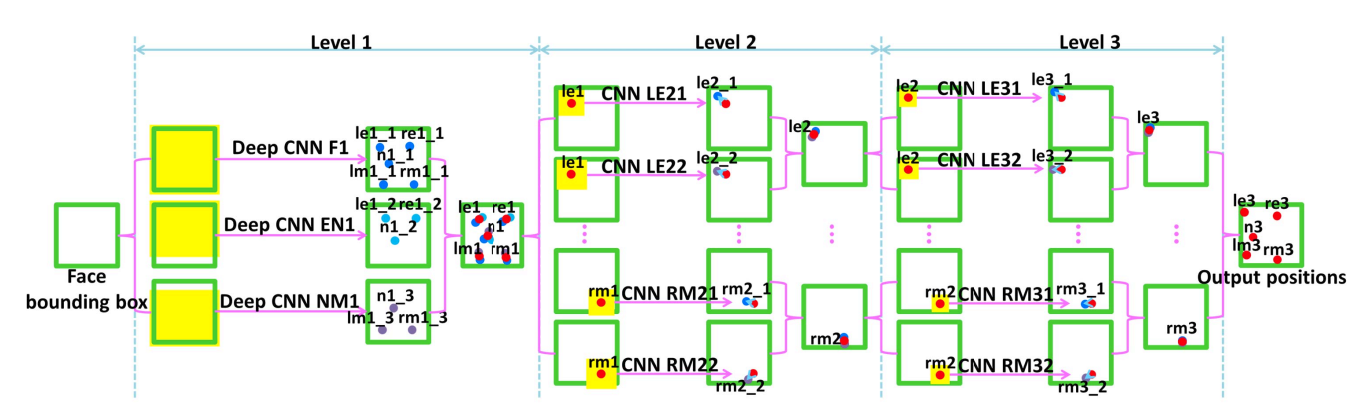
\includegraphics[scale=0.35]{images/3levels}
	\caption{The 3-levels proposed architecture}
	\label{3levels}
\end{figure}

At the first level, three CNNs are employed to study the location of the facial points: F1, EN1, NM1 whose input regions cover the whole face. F1 is studied all the position of five landmarks; EN1 is worked on the eyes and nose while NM1 worked on nose and the mouth corners. Each network predicts the landmarks corresponding with the region that it covers. At the end of level 1, the coordinate of each landmark is averaged of coordinates that predicted from three networks. Fig.\ref{1Fconv} illustrates the deep structure of the networks at level 1, which contains four convolutional layers followed by max pooling and two dense layers. F1, EN1, and NM1 take the same structure but with different size of the input and different output at full-connected layers to suitable with the number of predicted landmarks.
\begin{figure}[h]
	\centering
	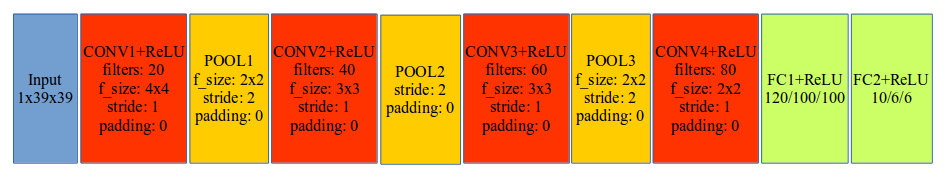
\includegraphics[scale=0.5]{images/cnn_level1}
	\caption{The structure of the networks in level 1}
	\label{1Fconv}
\end{figure}

The networks at the second and third levels take local patches centered at the predicted position of previous levels as input. Besides, they allowed to make small changes to previous prediction. The size of patches are also reduced along with the cascade model. For each position, two networks are used to predict the new positions. The last predicted position is average of the new positions. Fig.\ref{2lvconv} illustrates the architecture of the networks in level 2 and level 3. Basically, the networks in last two levels are similar, the only difference is the way to choose the patch around the landmark. A padding is added to the coordinates of the landmark to make the change of the patches i.e $0.16, 0.18$ in level 2 and $0.11, 0.12$ in level 3. Then, the patch is resized to the size of $15 \times 15$ before giving the networks.
\begin{figure}[h]
	\centering
	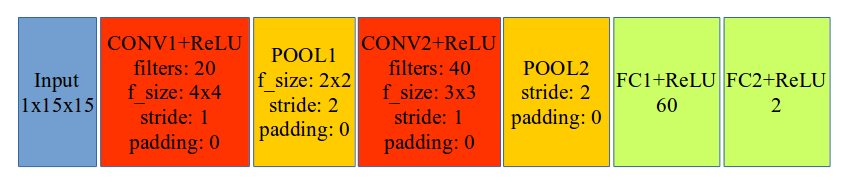
\includegraphics[scale=0.5]{images/cnn_level2}
	\caption{The structure of the networks in level 2, level 3}
	\label{2lvconv}
\end{figure}

 With 3-levels model, the purpose of the networks at the first level are estimated the landmark positions with large errors; the networks at last two levels are designed to achieve high accuracy.
\subsection{Experiments}
\subsubsection{Training}
At the first level, $F1$ takes the whole face as input (size of $39 \times 39$ of the network and outputs the position of all the five points. $EN1$ takes the top and middle part of face as input (size of $31 \times 39$) and outputs the positions of two eye centers and nose tip. $NM1$ takes the bottom and middle part of the face to predict the positions of nose tip and two corners of mouth.

All the networks at level 2 and level 3 take a small squares ($15 \times 15$)centered at the predicted position by the previous level as the input and output the incremental prediction. The last predicted positions at each level are average of corresponding positions from all the networks in each level. 

During training, the size of the patches is decreased for each level. The learnable parameters include weight w, the gain g and the bias b which are initialized by small random number and learned by stochastic gradient descent.

The detection error on each facial point is measured by Eq.\ref{eq1}. If the error is greater than $5\%$, it is considered as failure.
\begin{equation}
	err = \sqrt{(x-x')^2 + (y-y')^2}/l
	\label{eq1}
\end{equation}
Where:
\begin{itemize}
	\item l is the width of the bounding box around the face.
	\item $(x,y)$ is ground truth facial point
	\item $(x',y')$ is predicted position
\end{itemize}
\subsubsection{Testing}
The model is tested with a dataset of 2557 face images. The image with the bounding box of the face is used as the input of the model. At the end, the predicted position is estimated from the model. By using the way in Eq.(\ref{eq1}) to evaluate the model, the error statistic on each level is obtained (Figs. \ref{rslevel1}, \ref{rslevel2}, \ref{rslevel3}).
%\begin{table}[h!]
%	\centering
%	\begin{tabular}{c}
%	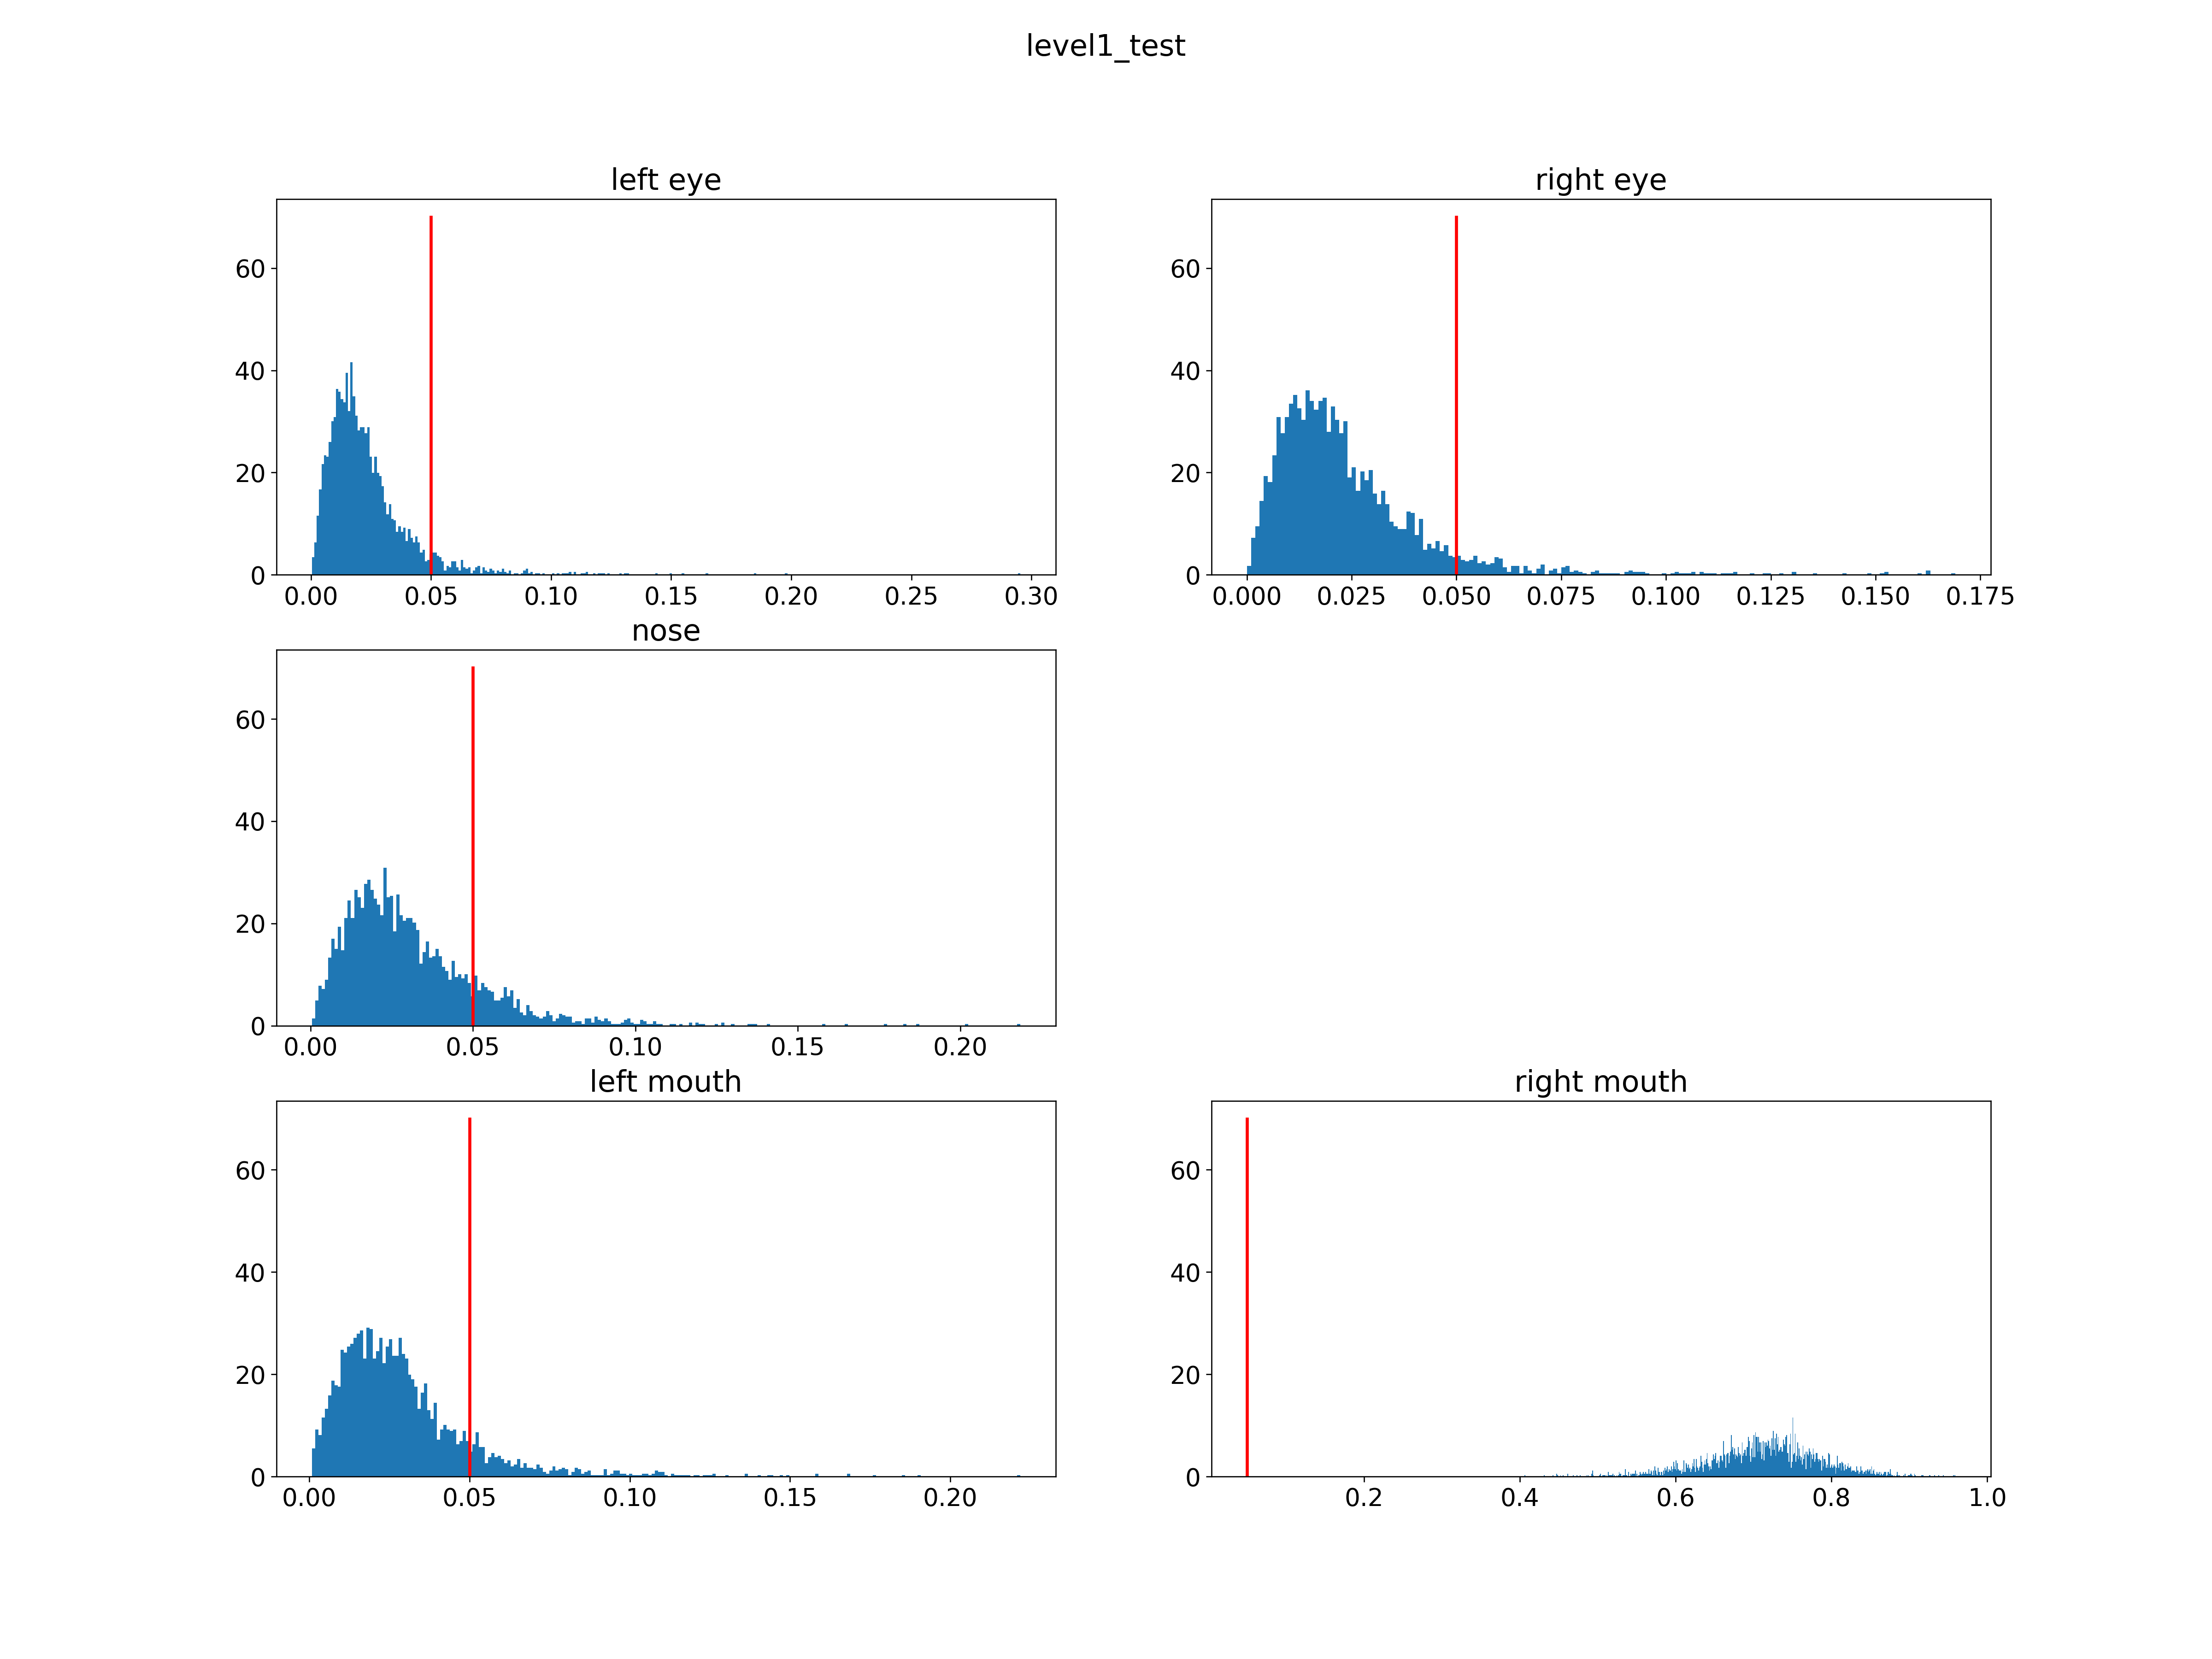
\includegraphics[scale=0.3]{images/level1_test}~\\
%	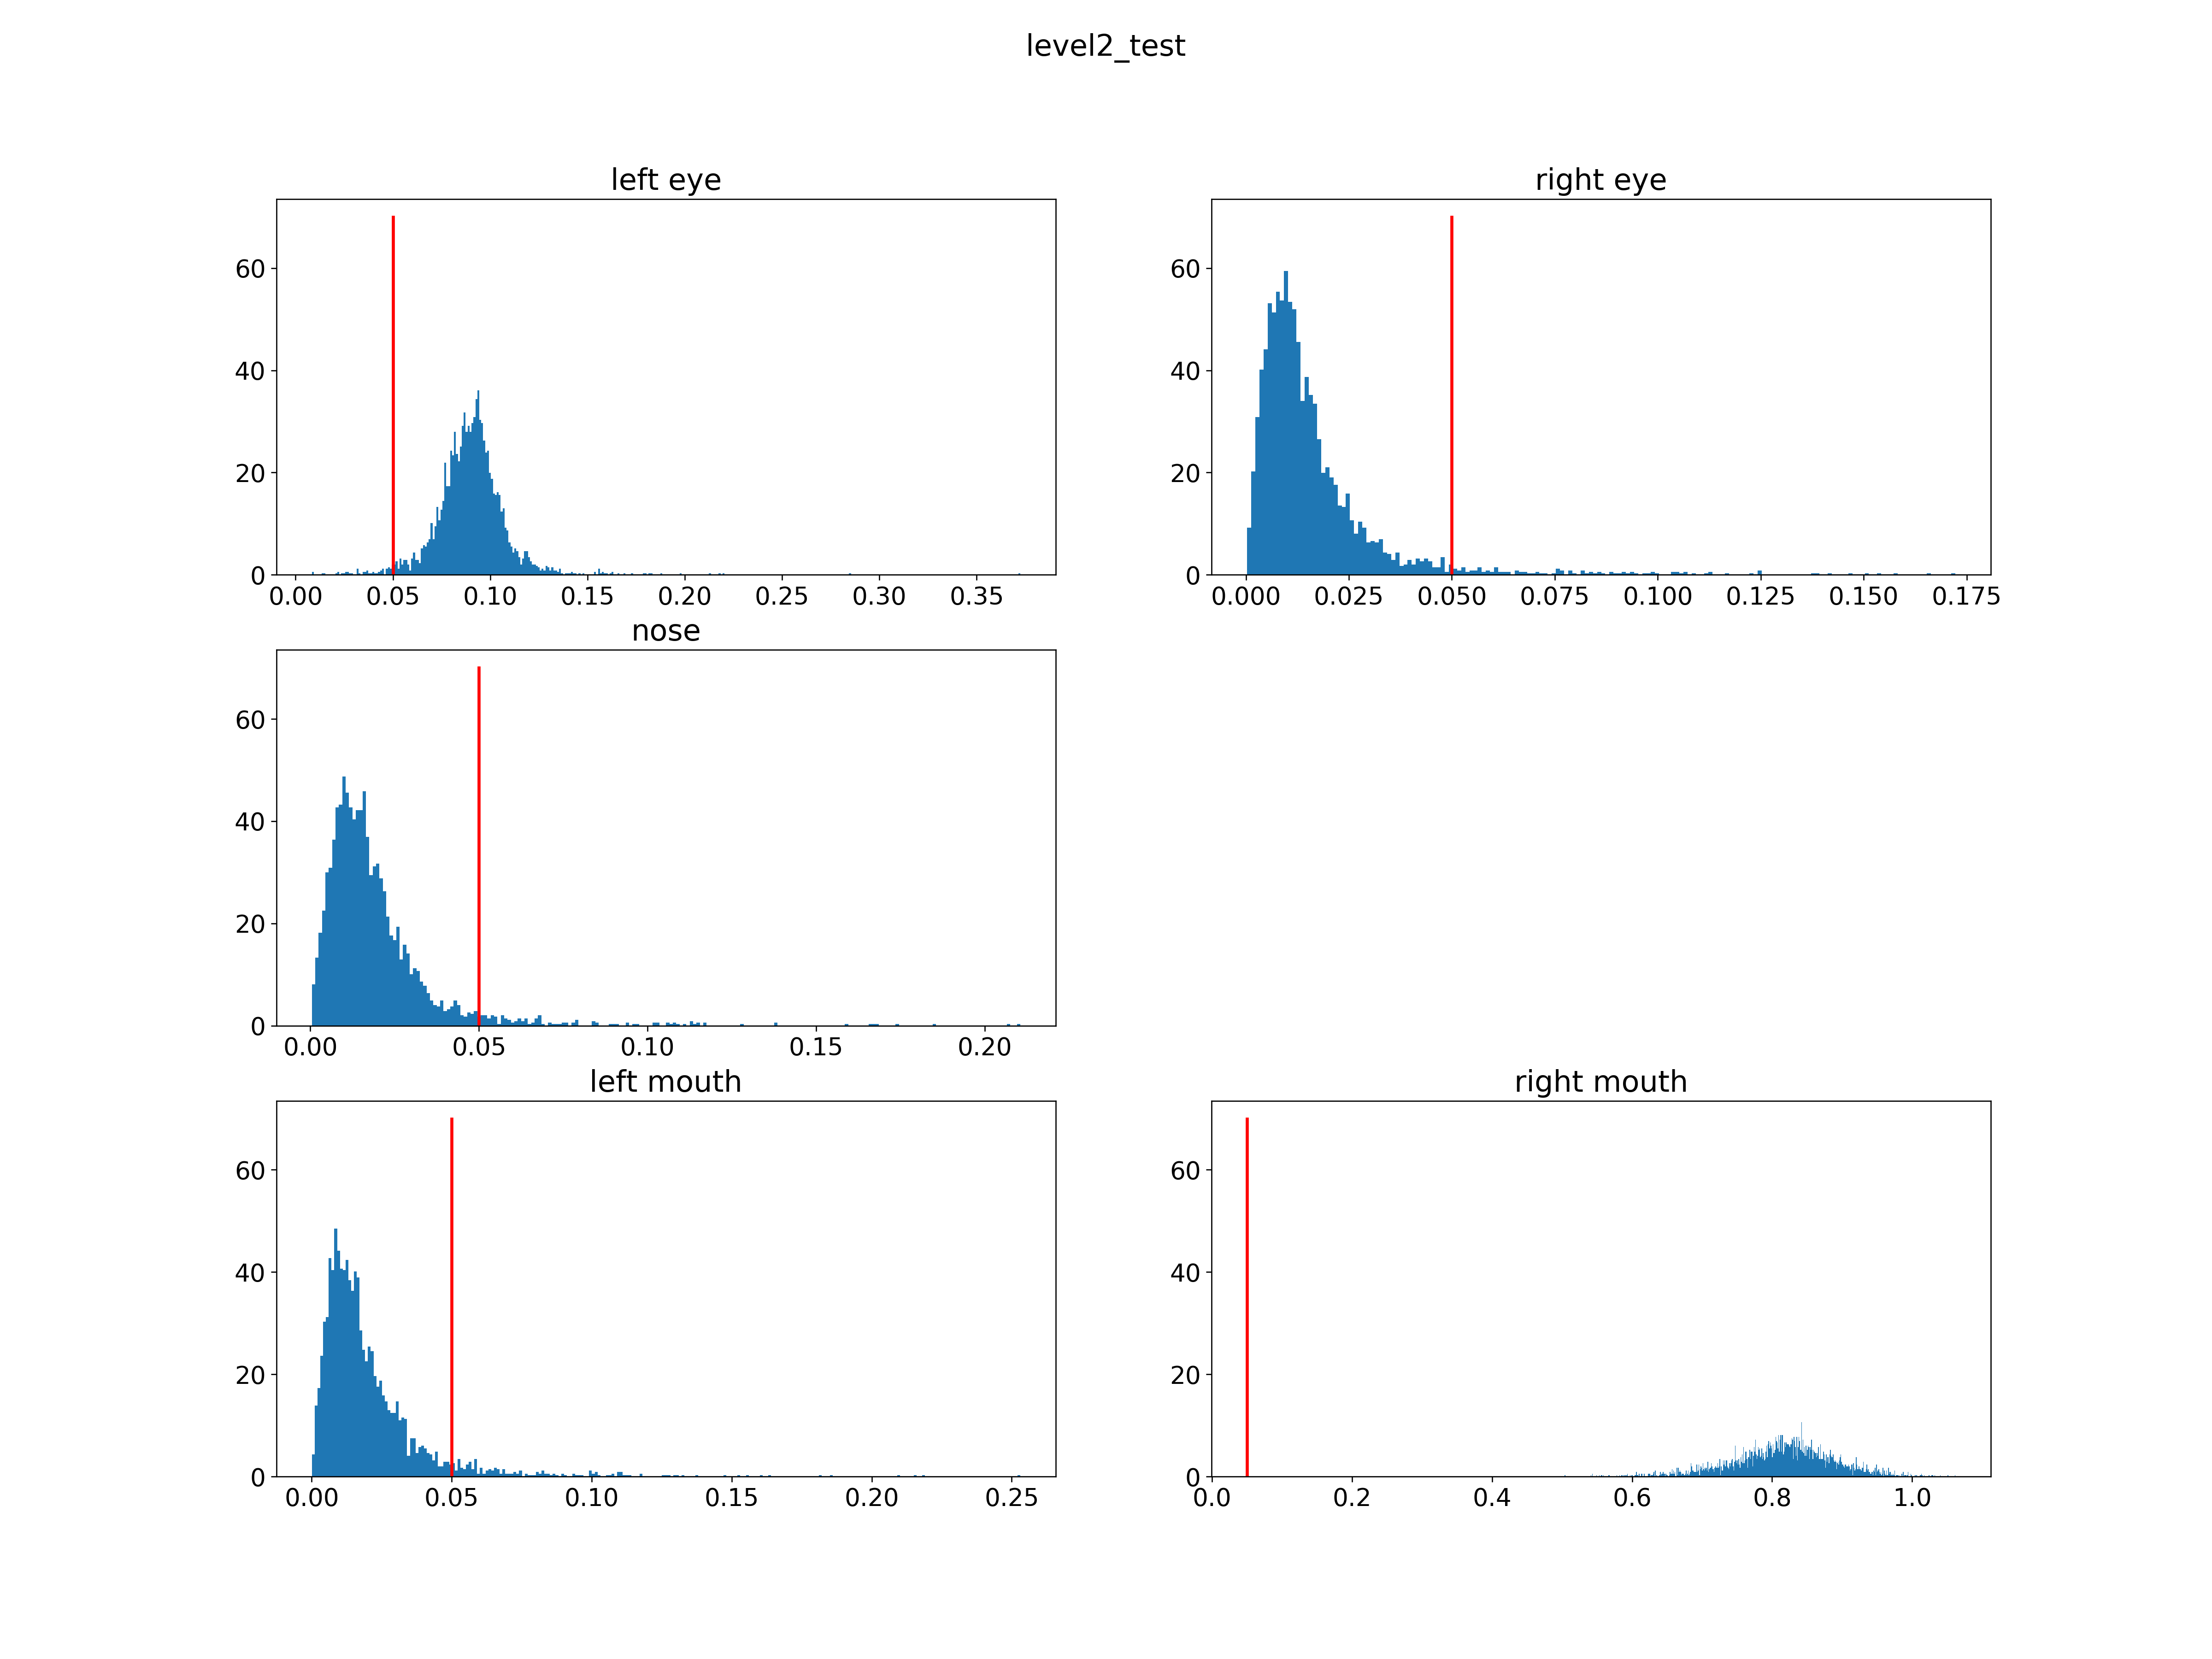
\includegraphics[scale=0.3]{images/level2_test}~\\
%	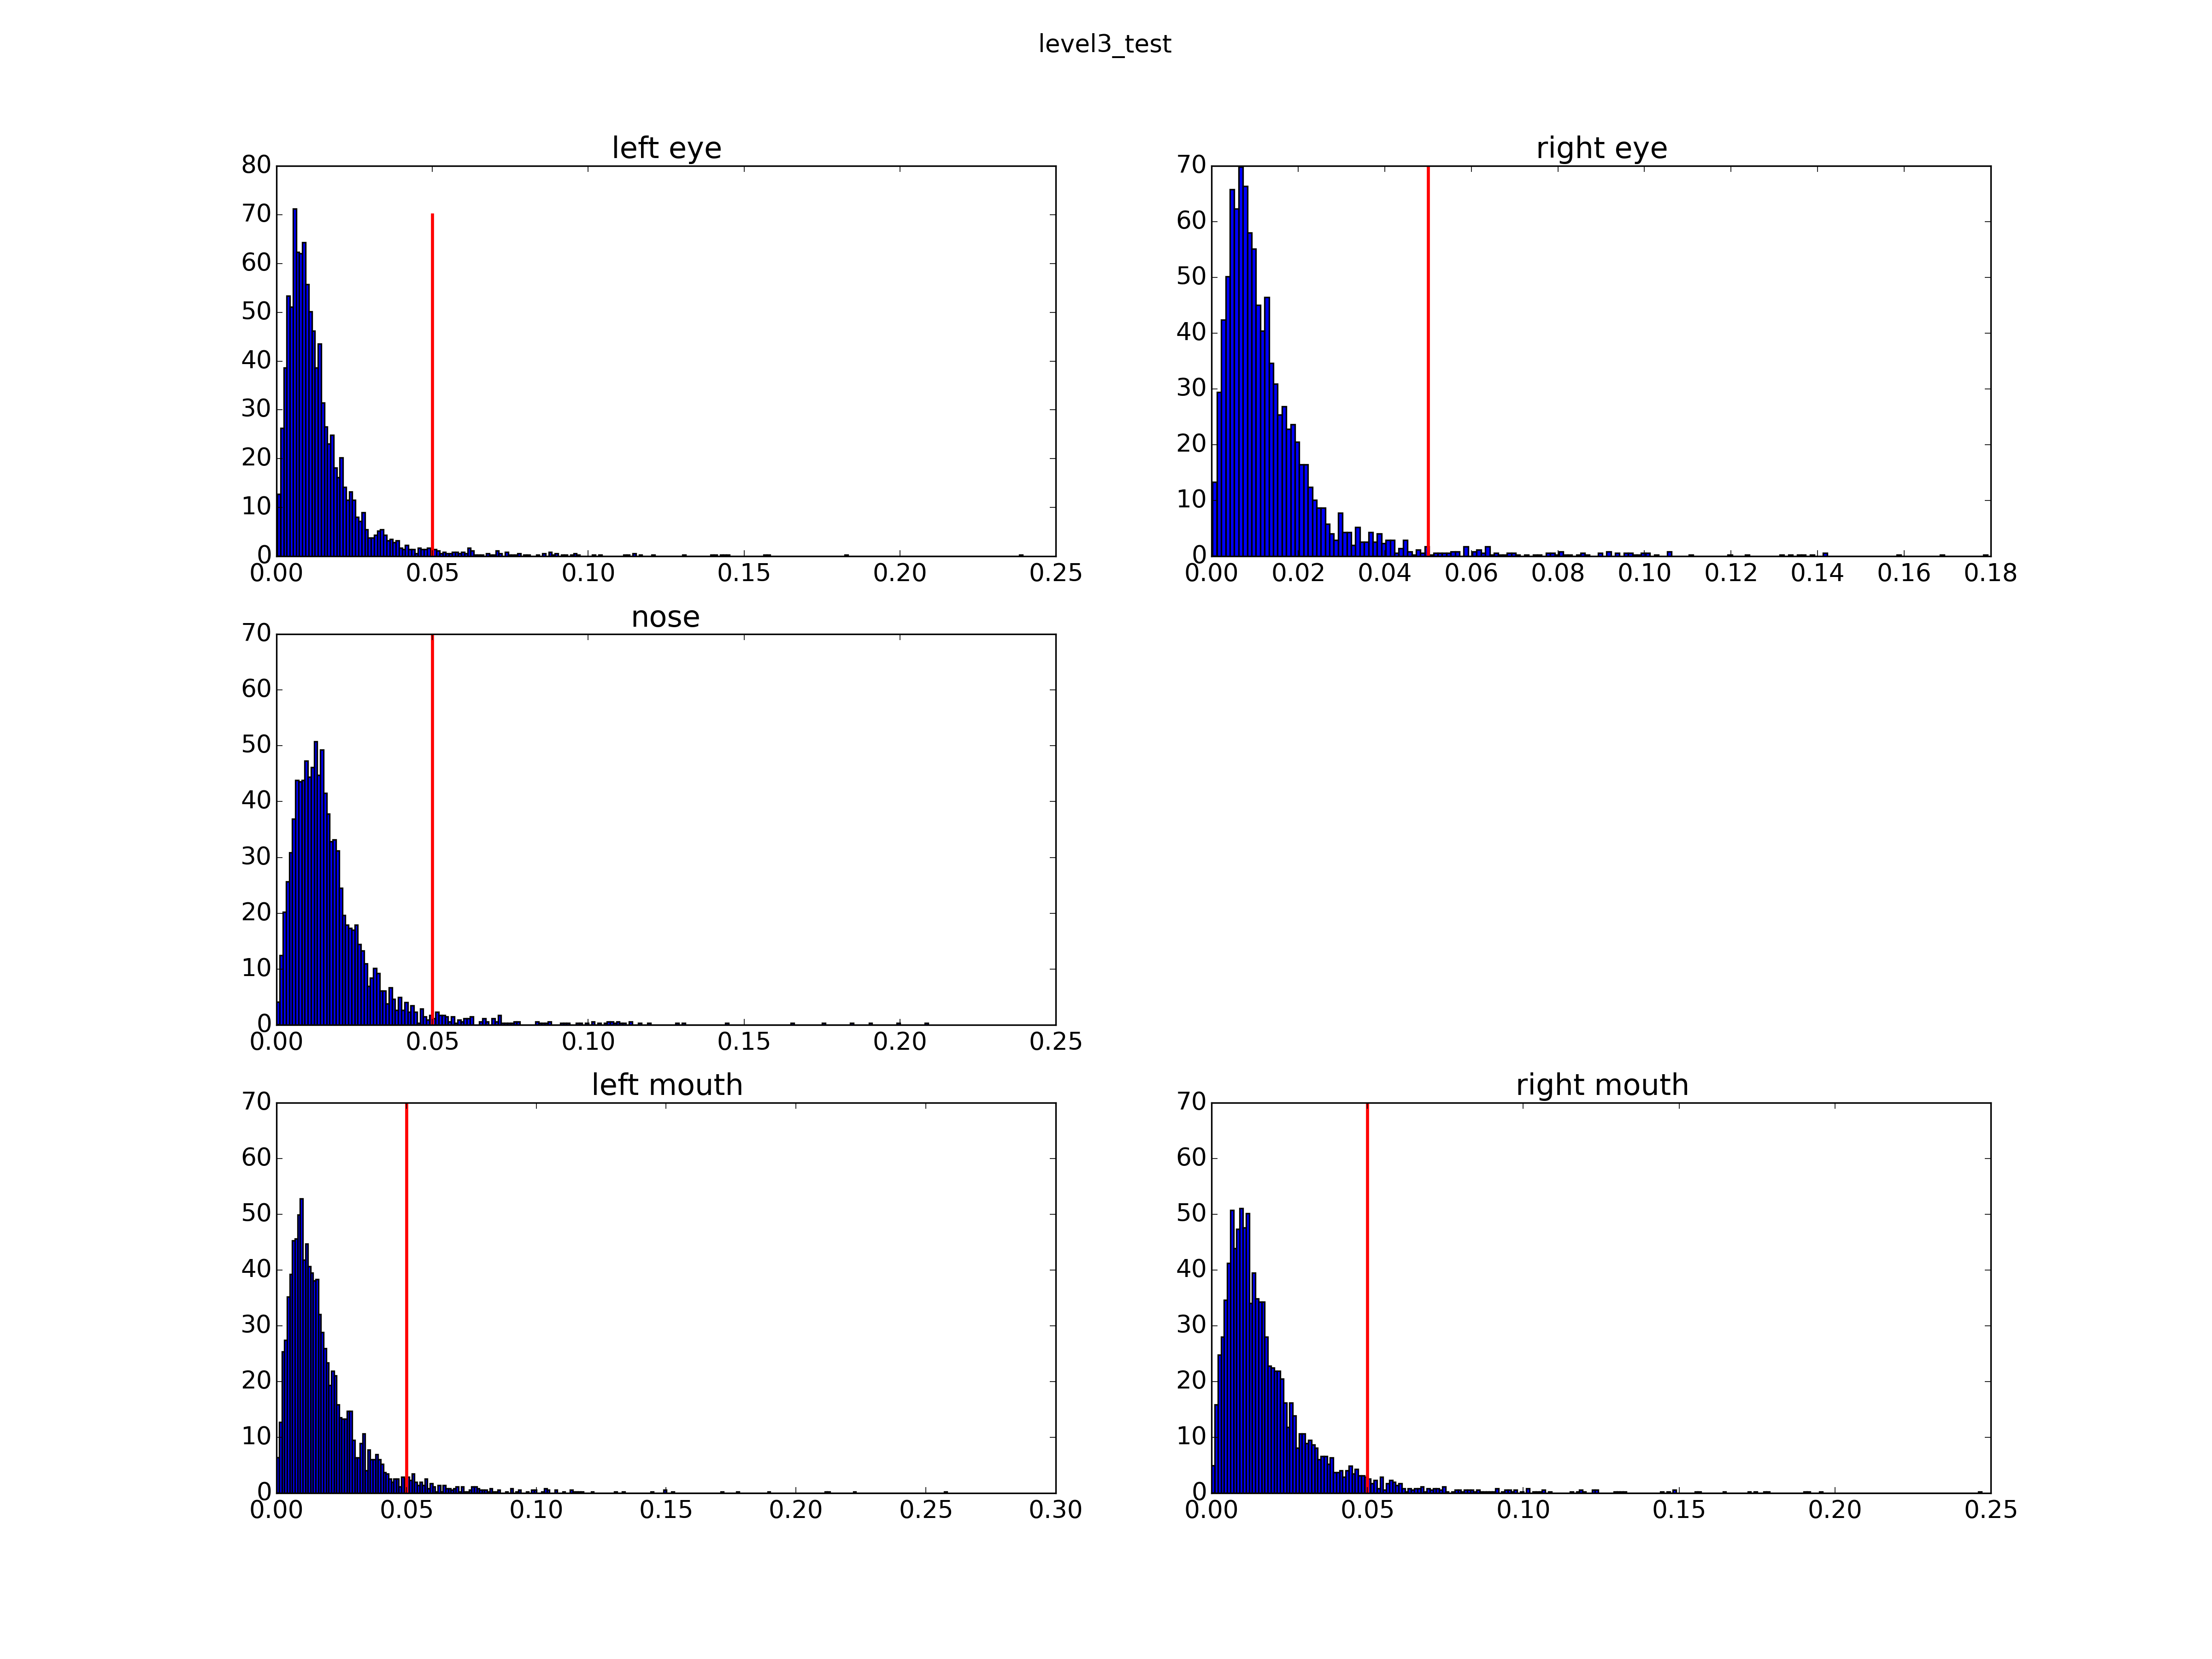
\includegraphics[scale=0.3]{images/level3_test}
%	\end{tabular}	
%\end{table}
\begin{figure}[h!]
	\centering
	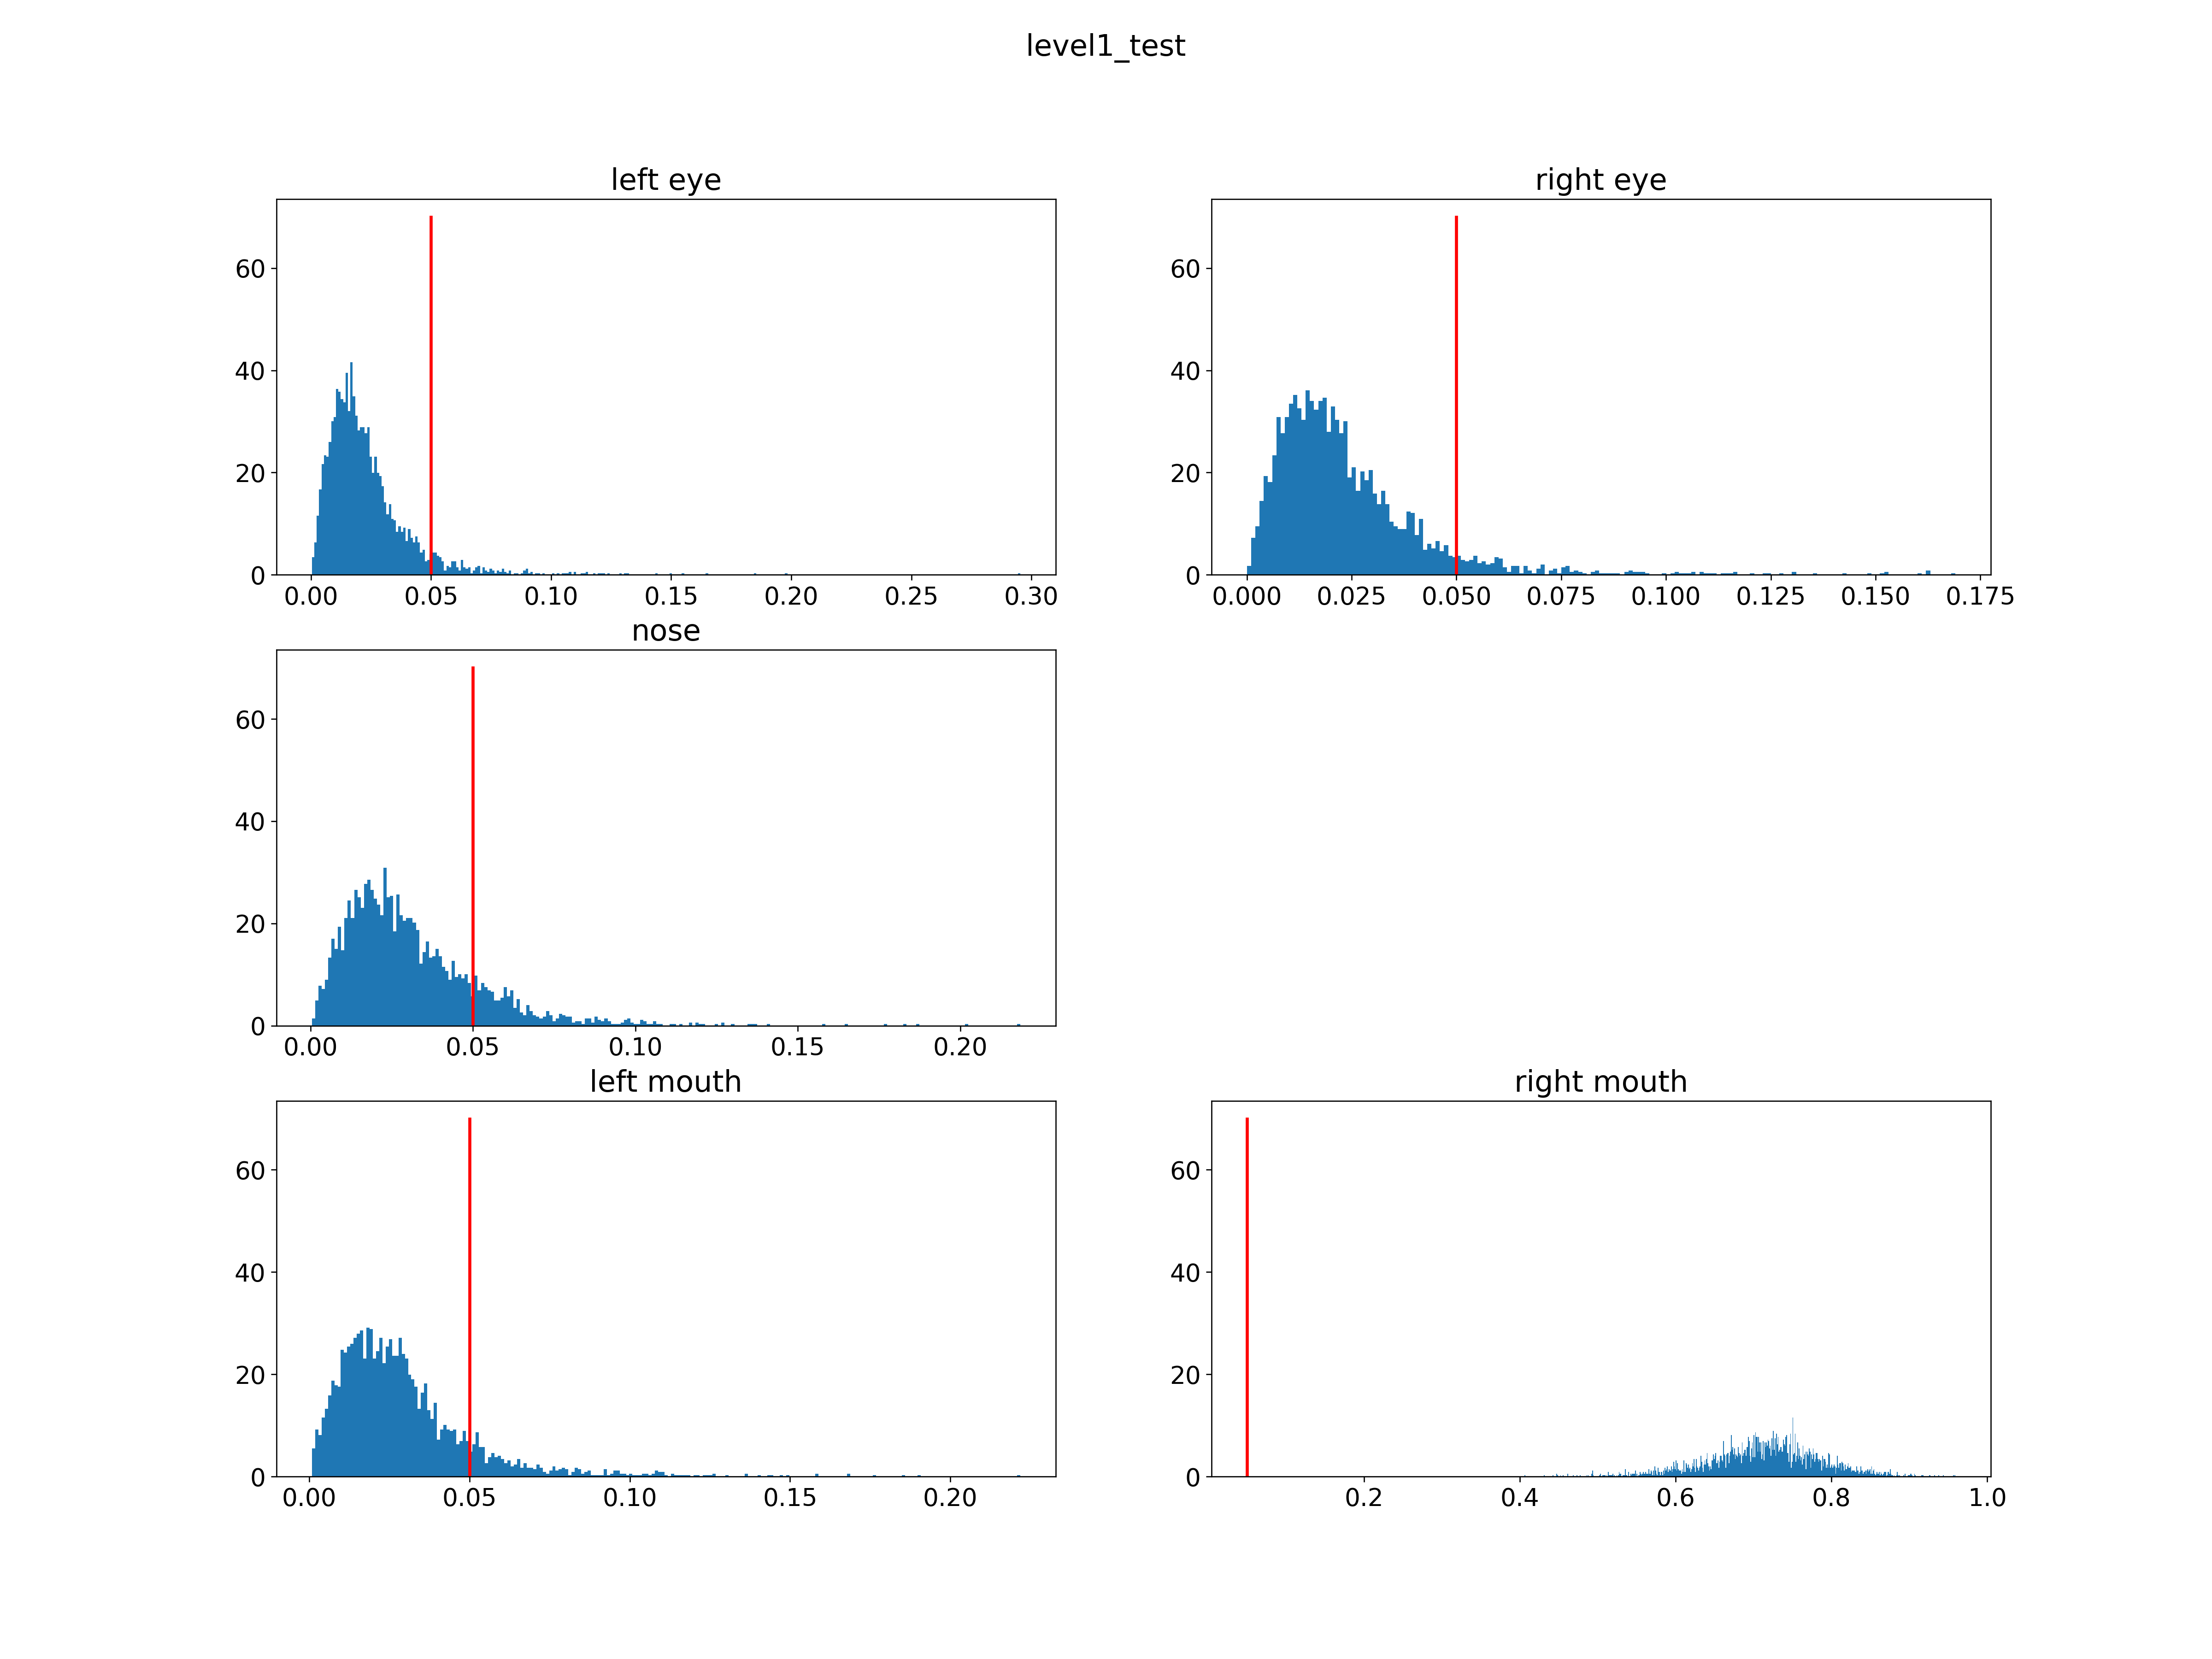
\includegraphics[scale=0.25]{images/level1_test}
	\caption{The error on each landmark in level 1}
	\label{rslevel1}
\end{figure}
\begin{figure}[h!]
	\centering
	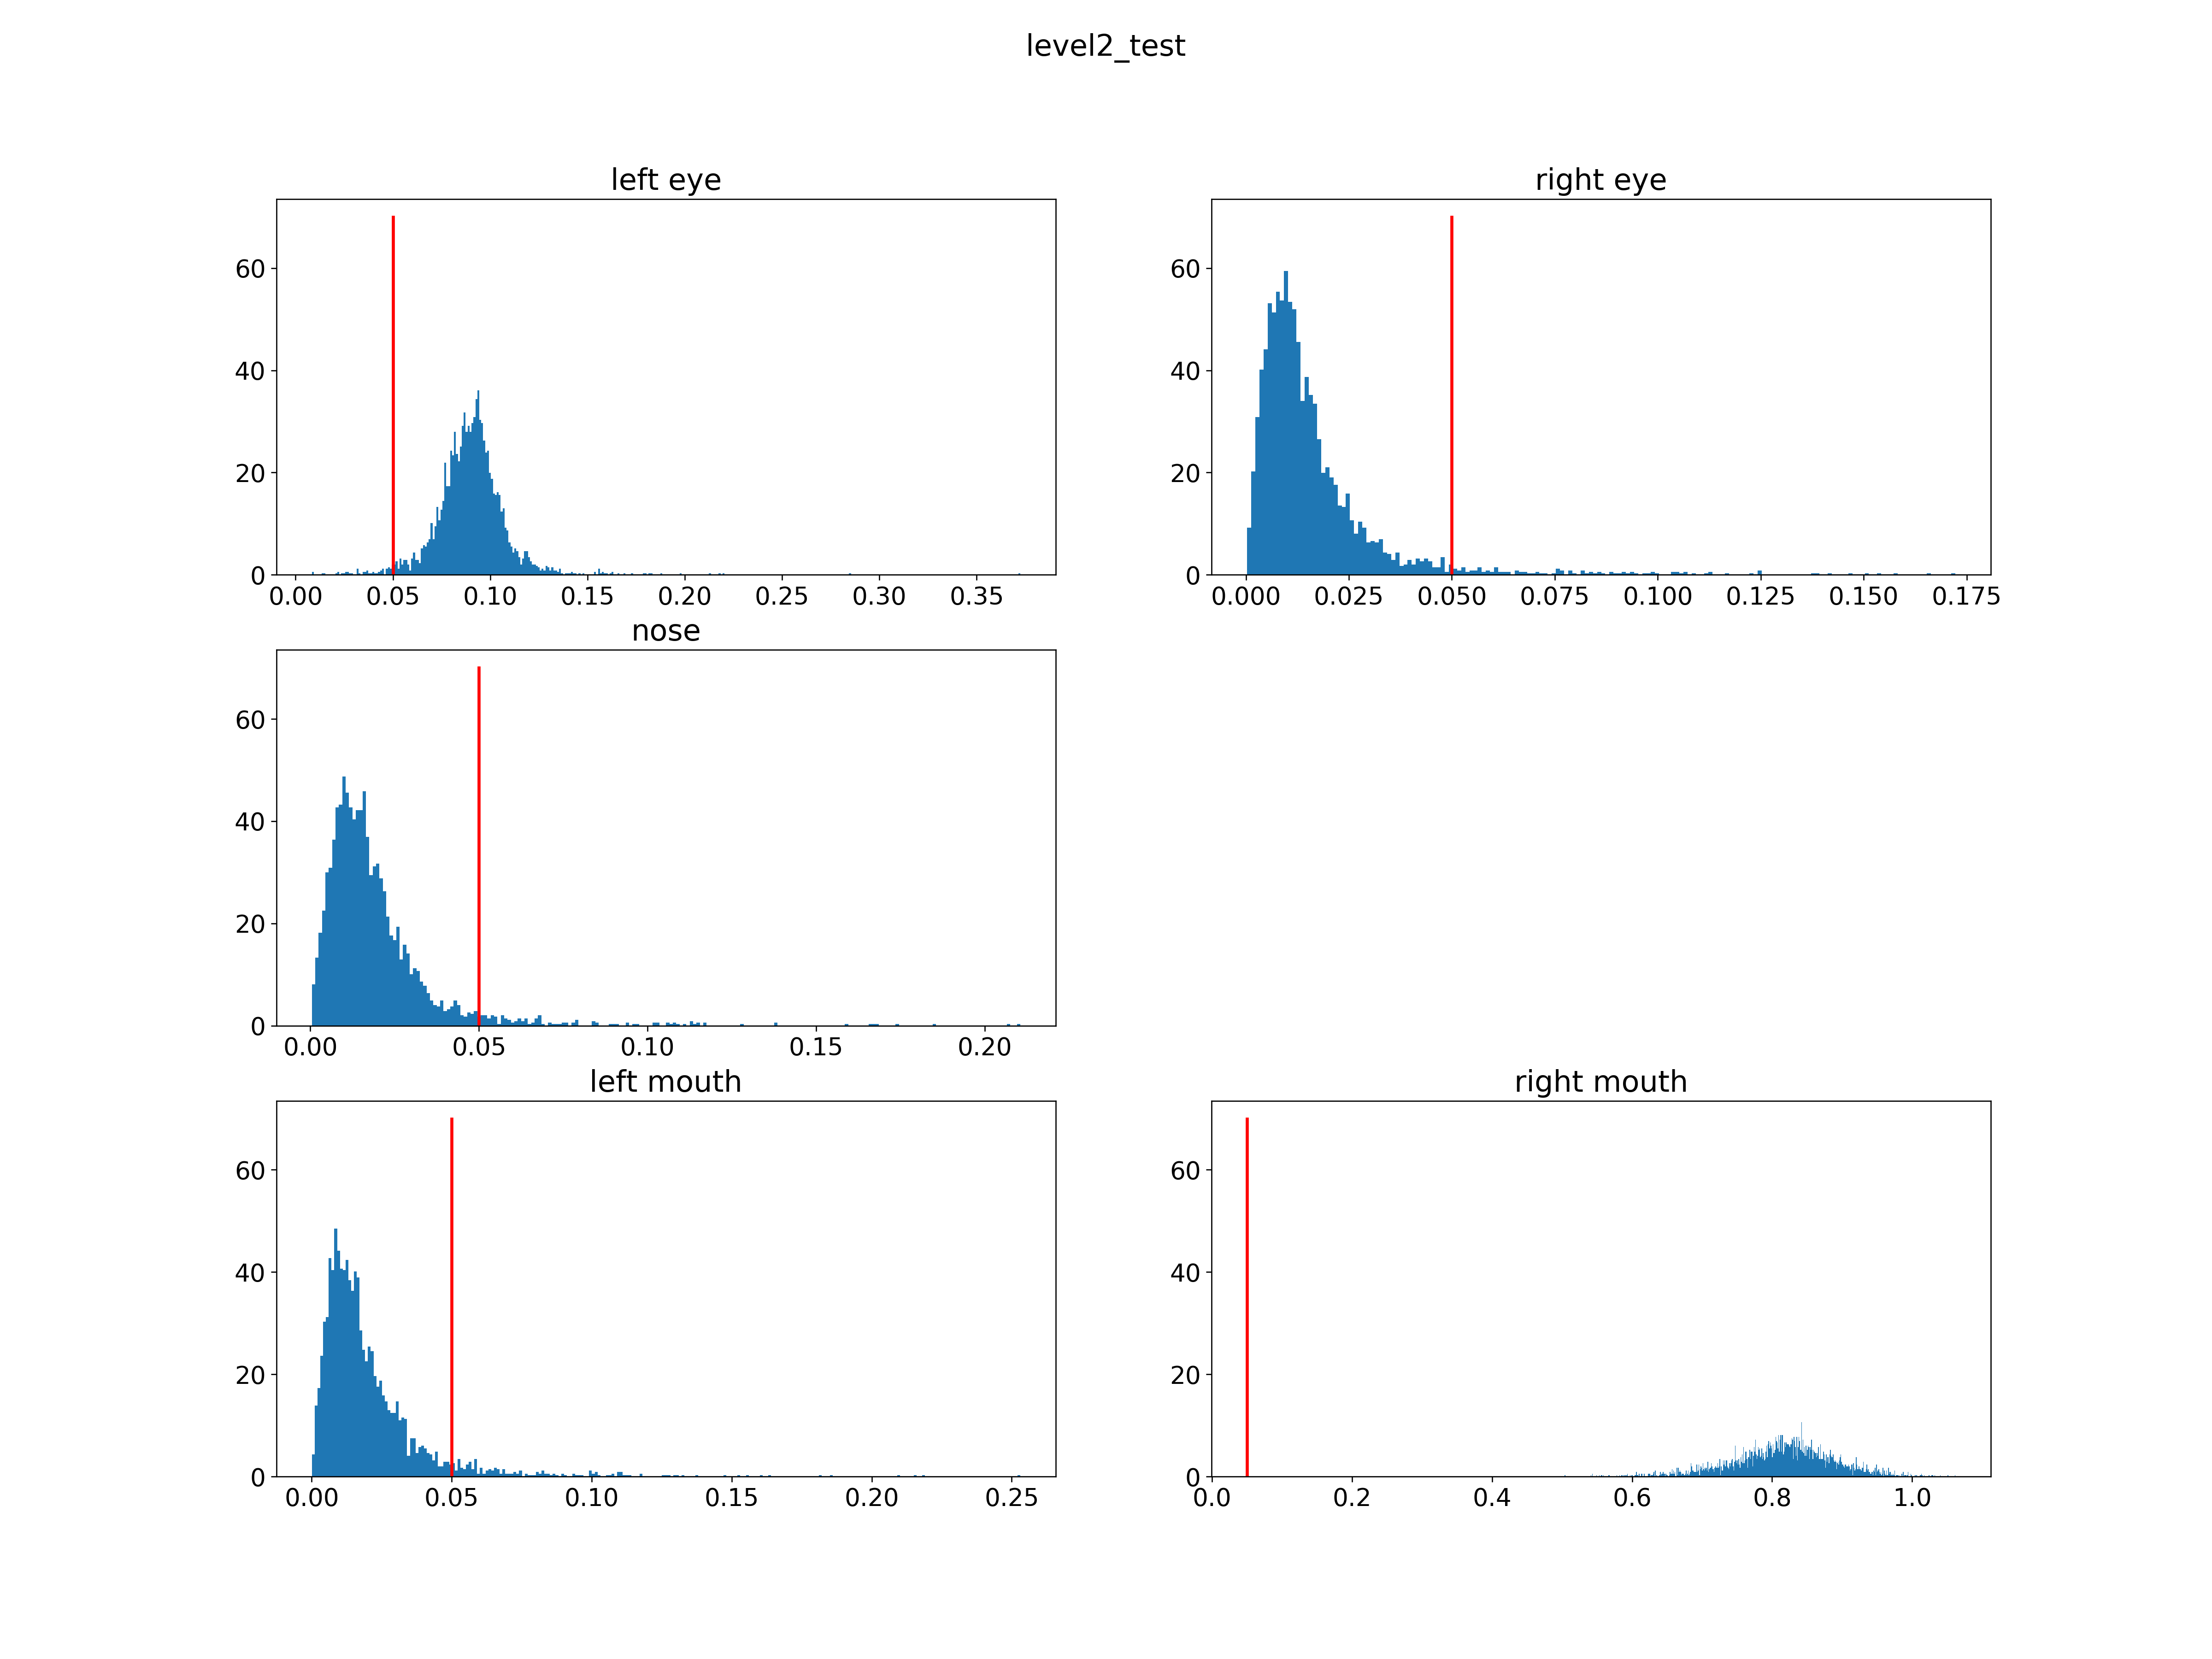
\includegraphics[scale=0.25]{images/level2_test}
	\caption{The error on each landmark in level 2}
	\label{rslevel2}
\end{figure}
	\begin{figure}[h!]
	\centering
	\includegraphics[scale=0.25]{images/level3_test}
	\caption{The error on each landmark in level 3}
	\label{rslevel3}
\end{figure}
\pagebreak
\section{Model 2: Automatic ear landmarks detection by CNN}
Celia Cintas et al\cite{cintas2016automatic} proposed a method based on geometric morphometric and deep learning for automatic ear detection and feature extraction in the form of landmarks. The convolutional neural network was trained with a set of manually landmarks examples. The network is able to provide the morphometric landmarks on ear image automatically.
\subsection{Dataset}
The image and manual landmarks belong to the CANDELA initiative \footnote{https://www.ucl.ac.uk/candela}, a project includes geneticists, bioinformatics and social-anthropologists interested on Latin American. CANDELA contains 7500 images with the size of $2136 \times 3216$. The provided dataset contains 2753 images which extracted from the CANDELA dataset. For each image, a set of 45 landmarks and semi-landmarks provided by human operators. The dataset was split into a training set with 2051 images (75\%) and a validation set of 684 images (25\%).
\subsection{Network}
Three models were designed and trained for performing the automatic landmarks task. These architectures are different in the number of convolution layers, the filter sizes, and the learning rate. An image with a single channel of the size  $96 \times 96$ with brightness scaled to $[0,1]$, is taken as the input of the network. The target (landmarks coordinates) is scaled to $[-1,1]$. \textbf{Fig.\ref{1Econv}} shows the best architecture. In this architecture, a structure of two convolutional layers with the filters, followed by maximum pooling and dropout layer. This structure is repeated three times to obtain features at different levels with different size of filters(i.e $4 \times 4$ and $3 \times 3$). After extraction the features, two fully connected linear layers with 1500 units each and a dropout layer is hired. The output layer contains 90 output units corresponding with 45 landmarks for the predicted position of the landmarks. The implementation used Python and the Lasagne library\cite{lasagne}.
\begin{figure}[h!]
	\centering
	\includegraphics[scale=0.4]{images/ear_cnn}
	\caption{The best architecture for automatic ear's landmarks detection}
	\label{1Econv}
\end{figure}
\subsection{Experiments}
%Following the article, the method is evaluated the usual quality metrics for regression problems, in particular $r^2$, root mean square error (RMSE), explained variance (EV), and Pearson's correlation.
%The accuracy of three architectures are shown in Table \ref{tbear1}. Also, in Table \ref{tbear2}, the RMSE for each landmarks is shown. The regression metrics were computed using \textit{scikit-learn}\cite{}.

%\begin{table}[h!]
%	\centering
%	\begin{tabular}{l c c c}
%	& Arch0 & Arch1 & Arch2 \\ \hline
%	$r^2$ & 0.709 & 0.678 & 0.698 \\ \hline
%	RMSE & 2.296 & 2.415 & 2.338\\ \hline
%	EV & 0.976 & 0.974 &  0.975 \\ \hline
%	Pearson & 0.988 & 0.987 &  0.988 \\ \hline	
%	\end{tabular}
%	\caption{Performance of three different ConvNet architectures}
%	\label{tbear1}
%\end{table}\\
%\begin{table}[h!]
%	\centering
%	\begin{tabular}{l r}
%	\# Landmark & RMSE \\ \hline
%	1 & 1.8183 \\ \hline
%	2 & 1.2216\\ \hline
%	3 &  1.08651\\ \hline
%	4 &  1.3291\\ \hline
%	5 &  2.4477\\ \hline
%	6 &  2.59746\\ \hline
%	7 &  1.17571\\ \hline
%	\end{tabular}
%	\caption{RMS error for each landmark}
%	\label{tbear2}
%\end{table}\\

Because the CANDELA dataset is not published. Another dataset was chosen to study the network. The new dataset was used for the Facial Keypoint Detection including 7049 gray-scale images ($96 \times 96$). For each image, we are supported learn to find the position of 15 landmarks. After dropping some missing data, the dataset remains 2140 images. All the images with coordinates of manual landmarks is stored in csv file and fetched into the network. During the training and validation, the usual quality metrics for regression problems is used, in particular, root mean square error (RMSE). Fig.\ref{earLosstrain} shows the learning curves of the model on training and validation set error. The training is finished after 3000 iterations with the loss arround $10^{-3}$.
\begin{figure}[h!]
	\centering
	\includegraphics[scale=0.27]{images/trainloss}
	\caption{The loss of Ear-CNN network on facial point dataset}
	\label{earLosstrain}
\end{figure}
Fig.\ref{earTest} shows some test on the real facial images.
\begin{figure}[h!]
	\centering
	\includegraphics[scale=0.27]{images/figure_1-1.png}
	\caption{The prediction landmarks on human face}
	\label{earTest}
\end{figure}
\section{Model 1 and model 2 on pronotum}
\subsection{Dataset preparing}
The dataset includes 293 pronotum images. The images are divided into three subsets: the training set (200 images), the validation set (60 images) and the testing set (33 images). Because the dataset is limited and the models are worked on gray-scale images, we applied some ways to en-large the dataset. Firstly, for each original image in RGB, each channel is modified by adding some values. Secondly, the channels of the original image are split. So, we have obtained 1400 images for the training set and 420 images for the validation set. At the end, the images are down-sampled with the  size of $256 \times 192$ before giving to the networks.

%To enlarge the dataset during training, the image in training and validation set are augmentation by modifying the valued of red and green channel. So, at the end, we have 600 and 180 images in training and validation set, respectively.
\subsection{Model 1 and pronotum landmarks}
The networks in the first level are modified to suitable with the prediction of landmarks on the pronotum (8-landmarks). For each pronotum, eight manual landmarks have been set. The bounding box is created depending on the coordinate of the manual landmark and kept with the same size. The networks in the first level are used as followed:
\begin{itemize}
	\item F1 network recognizes whole pronotum bounding box with eight landmarks.
	\item EN1 network predicts the location of the first five-landmarks i.e $[1..5]$.
	\item NM1 network is used to estimated the position of last four-landmarks and the first landmark i.e $[5..8,1]$.
	\item At the end, the position of each landmark is average of the predicted position in the networks.
\end{itemize} 
\subsubsection{Testing}
During training, the Euclidean distance (sum of squares) is used to compute the loss of the networks. The error rate of each network during training is shown in the Table.\ref{model1p}:\\
\begin{table}[h!]
	\centering
	\begin{tabular}{l r}
	Network & Loss \\ \hline
	F1 & 0.013 \\ \hline
	EN1 & 0.47\\ \hline
	NM1 &  0.5
	\end{tabular}
	\caption{The loss of the networks in Model 1 on pronotum dataset}
	\label{model1p}
\end{table}
\begin{figure}[h!]
\centering
\subfloat[Test 1]{\label{}\includegraphics[width=0.2\textwidth]{./images/test1}}~~
\subfloat[Test 2]{\label{}\includegraphics[width=0.2\textwidth]{./images/test2}}\\
\subfloat[Test 3]{\label{}\includegraphics[width=0.2\textwidth]{./images/test3}}~~
\subfloat[Test 4]{\label{}\includegraphics[width=0.2\textwidth]{./images/test4}}\\
\caption{The pronotum with predicted landmarks at level 1}
\label{model1pTest}
\end{figure}\\
From Table \ref{model1p}, the errors of EN1 and NM1 are still high. That errors make the prediction result of level 1 do not enough good. Besides, the networks at level 2 and level 3 used the prediction at level 1 as the input data to predict the new position. So, we can not continue with the level 2, 3 until the result at level 1 is improved. Perhaps, the model in model 1 is not suitable to detect the landmarks on pronotum.  Fig. \ref{model1pTest} shows the prediction landmarks on four images. Followed that, the networks can detect the landmarks at positions 4, 5 and 7; the different positions still not good.
\subsection{Model 2 and pronotum landmarks}
The dataset is kept the same with model 1 (1400 images for training and 420 images for validation) but having some changes. Firstly, the ways to choose the data(to train and validate) is changed. All images are combined. Then, the network will automatically choose $75 \%$ data to train and $25 \%$ for validation. Secondly, the inputs that given to the network are just the image and landmarks(without the coordinates of the bounding box).

The network is run 3000 iterations with the learning rate begin from $0.08$ to $0.01$. During training, the learning rate is changed to fit with the remaining iterations\cite{lecun2012efficient}. Fig.\ref{model2pl} shows the first 700 iterations during training. The loss did not have many changes after $100^{th}$ iteration.

\begin{figure}[h!]
	\centering
	\includegraphics[scale=0.4]{images/figure_1_loss_celia}
	\caption{The losses of model 2 on pronotum dataset}
	\label{model2pl}
\end{figure}

\begin{figure}[h!]
	\centering
	\includegraphics[scale=0.25]{images/figure_1_celia}
	\caption{The prediction landmarks on pronotum of model 2}
	\label{model2pt}
\end{figure}
Fig.\ref{model2pt} shows the prediction landmarks on 16 images. Following, the prediction landmarks from the network of model 2 are closed with the pronotum but the location is still inaccurate.

%\subsection{Comparing model 1 and model 2}
%Table C shows some differences from 2 models
%\begin{table}[h!]
%	\centering
%	\begin{tabular}{l c c c}
%	Model & Framework & Dataset (images) & Learning rate \\ \hline
%	Model 1 & Caffe & 13466 & 0.013 \\ \hline
%	Model 2 & Lasagne(Theano) & 2140 & zz\\
%	\end{tabular}
%\end{table}\\
\section{Proposed architecture (model 3)}
\subsection{Model and parameters}
From the tutorial of Daniel Nouri\footnote{http://danielnouri.org/} about using CNN to detect facial key points. We propose a CNN to detect the landmarks on pronotum. The proposed network includes three convolutional layers followed by three maximum pooling layers and three full connected layers(Fig.\ref{pmodel}). The network receives the gray-scale image ($256 \times 192$) as the input. The deep of convolutional layers is increased from $32, 64, $ to $ 128$ with different size of filter. The size of filters in pooling layers are kept in the same size of $2 \times 2$. At the end of network, three full-connected layers with the size of $500, 500, $ and $16$ are set up to predict the positions of landmarks. Besides, the model is designed with a small sharing learning-rate and the momentum. The learning-rate and the momentum are changed overtime of training.
\begin{figure}[h!]
	\centering
	\includegraphics[scale=0.4]{images/model3}
	\caption{The architecture of proposed model}
	\label{pmodel}
\end{figure}
\subsection{Training and experiments}
The model is trained with 1820 images in 5000 iterations. The images are normalized before giving to the network by scaling the intensity value to [0,1], instead of 0 to 255. The target values (x and y coordinates) is kept as original. During the training, the root-mean-square error (MSE) is used to calculate the loss.

To evaluate the stability and confidence of the model, we proposed several rules to select the images for the network, as Table.\ref{choosedata}:\\
\begin{table}[h!]
	\centering
	\begin{tabular}{c l l}
	Rule & Test set & Training and validation set \\ \hline
	rule\_1 & From $1^{st}$ image to $33^{rd}$ image & Remaining images \\ \hline
	rule\_2 & From $260^{th}$ image to $293^{rd}$ image & Remaining images\\ \hline
	rule\_3 & Random & Random \\ \hline
	rule\_4 & From $90^{th}$ image to $122^{nd}$ image & Remaining images\\ \hline
	rule\_5 & From $200^{th}$ image to $232^{nd}$ image & Remaining images \\ \hline
	\end{tabular}
	\caption{The rules to choose the data for the network}
	\label{choosedata}
\end{table}~\\
Following the rules to choose the data, the loss of training and validation is shown in Table \ref{losschoosedata}. From the results in the table, the training losses in the cases of \textit{rule\_4, rule\_5} are smaller than other rules; but the validation losses are stability. It means the overfitting is appeared clearly in the case of \textit{rule\_4} and \textit{rule\_5}. In which, the smallest difference value between training and validation loss is belong to \textbf{random} case.
\begin{table}[h!]
	\centering
	\begin{tabular}{c l l}
	Rule & Training loss & Validation loss \\ \hline
	rule\_1 & $0.12739$ & $0.63681$ \\ \hline
	rule\_2 & $0.15204$ & $0.59480$ \\ \hline
	rule\_3 & $0.16694$ & $0.55584$ \\ \hline
	rule\_4 & $0.08798$ & $0.61934$ \\ \hline
	rule\_5 & $0.0918$ & $0.52843$ \\ \hline
	\end{tabular}
	\caption{The training loss and validation loss following each rule to choose the data}
	\label{losschoosedata}
\end{table}~\\[0.1cm]
Fig.\ref{cnn3l} shows the training curve loss and validation curve loss of the model on each rule to choose the data. From the beginning, the loss is not changed. When the training is longer and the learning rate is improved, the loss is decreased and a large distance between training and validation is appeared (over-fitting) but it is not that bad.

The model is tested on the test datasets(five rules). Then, correlation between the manual landmarks and predicted landmarks is computed by applying the correlation methods (see Table.\ref{pearson}, \ref{spearman}, \ref{kendall})
\begin{table}[h!]
	\centering
	\begin{tabular}{c c c}
		Rule & x correlation & y correlation \\ \hline
		rule\_1 & $0.9953877$ & $0.9941767$ \\ \hline
		rule\_2 & $0.9968787$ & $0.9960827$ \\ \hline
		rule\_3 & $0.9966784$ & $0.9957729$ \\ \hline
		rule\_4 & $0.9975662$ & $0.9985097$ \\ \hline
		rule\_5 & $0.9972048$ & $0.9976416$ \\ \hline
	\end{tabular}
	\caption{The correlation between manual and predicted landmarks by Pearson\cite{pallant2013spss} method}
	\label{pearson}
\end{table}
\begin{table}[h!]
	\centering
	\begin{tabular}{c c c}
		Rule & x correlation & y correlation \\ \hline
		rule\_1 & $0.9893943$ & $0.9289319$ \\ \hline
		rule\_2 & $0.992556$ & $0.9444423$ \\ \hline
		rule\_3 & $0.9913126$ & $0.9565425$ \\ \hline
		rule\_4 & $0.9943106$ & $0.9789221$ \\ \hline
		rule\_5 & $0.9920646$ & $0.9864683$ \\ \hline
	\end{tabular}
	\caption{The correlation between manual and predicted landmarks by Spearman\cite{myers2010research} method}
	\label{spearman}
\end{table}
\begin{table}[h!]
	\centering
	\begin{tabular}{c c c}
		Rule & x correlation & y correlation \\ \hline
		rule\_1 & $0.913517$ & $0.7498531$ \\ \hline
		rule\_2 & $0.9303295$ & $0.8231899$ \\ \hline
		rule\_3 & $0.9273002$ & $0.8273057$ \\ \hline
		rule\_4 & $0.9419902$ & $0.8904413$ \\ \hline
		rule\_5 & $0.9299128$ & $0.9051508$ \\ \hline
	\end{tabular}
	\caption{The correlation between manual and predicted landmarks by Kendall\cite{kendall1938new} method}
	\label{kendall}
\end{table}

\begin{figure}[h!]
\centering
\subfloat[rule\_1]{\label{}\includegraphics[width=0.4\textwidth]{./images/figure_1_cnn3_5000_loss_v11}}~~
\subfloat[rule\_2]{\label{}\includegraphics[width=0.4\textwidth]{./images/figure_1_cnn3_5000_loss_v12}}\\
\subfloat[rule\_3]{\label{}\includegraphics[width=0.4\textwidth]{./images/figure_1_cnn3_5000_loss_v13}}\\
\subfloat[rule\_4]{\label{}\includegraphics[width=0.4\textwidth]{./images/figure_1_cnn3_5000_loss_v14}}~~
\subfloat[rule\_5]{\label{}\includegraphics[width=0.4\textwidth]{./images/figure_1_cnn3_5000_loss_v15}}
\caption{The loss during training and validation followed each rule to choose data }
\label{cnn3l}
\end{figure}
\pagebreak

Fig.\ref{cnn3t} show the predicted positions on test dataset followed rule\_3:
%\begin{figure}[h!]
%	\centering
%	\includegraphics[scale=0.2]{images/figure_1_loss_cnn3_3000_2}
%	\caption{The loss during training and validation of rule\_1}
%	\label{cnn3l}
%\end{figure}
\begin{figure}[h!]
	\centering
	\includegraphics[scale=0.2]{images/figure_1_cnn3_5000_v13}
	\caption{The prediction landmarks on 16-pronotum images}
	\label{cnn3t}
\end{figure}~\\[2cm]
%\begin{figure}[h!]
%	\centering
%	\includegraphics[scale=0.25]{images/plandmark}
%	\caption{The prediction landmarks on a pronotum}
%	\label{cnn3t1}
%\end{figure}
The network in model 3 is applied to predict the landmarks on tete and elytre with some modifications such as: the output at the last of full connected layer. The data that used to train and test are chosen by applying rule\_3. Table.\ref{tete},\ref{elytre} shown the statistic on the test set of tete and elytre by different correlation coefficient methods:
\begin{table}[h!]
	\centering
	\begin{tabular}{l c c}
		Method & x correlation & y correlation \\ \hline
		Pearson & $0.99082758$ & $0.988833$ \\ \hline
		Spearman & $0.9868292$ & $0.989447$ \\ \hline
		Kendall & $0.905933$ & $0.9130359$ \\ \hline
	\end{tabular}
	\caption{The correlation between manual and predicted landmarks on tete images}
	\label{tete}
\end{table}
\begin{table}[h!]
	\centering
	\begin{tabular}{l c c}
		Method & x correlation & y correlation \\ \hline
		Pearson & $0.984969$ & $0.9976646$ \\ \hline
		Spearman & $0.9840307$ & $0.966091$ \\ \hline
		Kendall & $0.8996806$ & $0.846849$ \\ \hline
	\end{tabular}
	\caption{The correlation between manual and predicted landmarks on elytre images}
	\label{elytre}
\end{table}~\\
From the result of Table \ref{losschoosedata}, the dataset which was chosen by rule\_3 is used to continue the experiments. To improve the results, we have modified the rule to pre-process the input data: the target (coordinates of manual landmarks) is normalized into the range of $[-1,1]$, instead of $[0,256]$ for x-coordinate and $[0,192]$ for y-coordinate. Additional, the \textit{learning rate} of the network has been changed to increase the speed of training process.

After changing, the result that we obtain as we expect: training loss and validation loss have decreased significantly(training loss: \textbf{0.00002}, validation loss: \textbf{0.00012}). Thus, the landmarks coordinates have been normalized into $[-1,1]$, so, to calculate the MSE error, we will take the square error and multiply by scale ratio again: the error is arround $1.4$(validation loss). Fig.\ref{tvlscaletarget} shows the losses during training and validation. We can see that overfitting have appeared during the train and validation processes.
\begin{figure}[h!]
	\centering
	\includegraphics[scale=0.5]{images/figure_1_cnn3_3000_v13_loss_change2}
	\caption{The training and validation loss when normalize the landmarks coordinates}
	\label{tvlscaletarget}
\end{figure}~\\
To prevent the overfitting on the network, we have modified both data and model: on data side, we have changed the \textit{split} ratio to get more samples for validation set($40\%$ instead of $20\%$ of number of samples); on model side, the number of units in the last two hidden layers (full-connected layer) are increased from 500 to 1000. Besides, four dropout layers have been added into the network. They have been located following the pooling layers and the first full-connected layer. The dropout ratios are $0.1$, $0.2$, $0.3$ and $0.5$ (Fig.\ref{model3dropout}).
\begin{figure}[h!]
	\centering
	\includegraphics[scale=0.35]{images/model3_dropout}
	\caption{The proposed model with dropout layers}
	\label{model3dropout}
\end{figure}~\\
Fig.\ref{tvldropout} shows the losses after the model have been modified. The overfitting problem is solved but the losses are stability from $2000^{th}$ until the end(we need more data). Table.\ref{coffdropout} shows the correlation coefficient of new model. Clearly that, the result have been improved a little bit when we compare with the last result. 
\begin{figure}[h!]
	\centering
	\includegraphics[scale=0.2]{images/figure_1_cnn3_3000_v13_loss_change3_dropout_increase_2}
	\caption{The training and validation loss with dropout layers}
	\label{tvldropout}
\end{figure}~\\
\begin{table}[h!]
	\centering
	\begin{tabular}{l c c}
		Method & x correlation & y correlation \\ \hline
		Pearson & $0.9970585$ & $0.9978605$ \\ \hline
		Spearman & $0.9942475$ & $0.9859642$ \\ \hline
		Kendall & $0.9430501$ & $0.9067739$ \\ \hline
	\end{tabular}
	\caption{The correlation between manual and predicted landmarks on pronotum images with new model}
	\label{coffdropout}
\end{table}
\section{Conclusions}
In this studied, two methods that used to predict the landmarks on 2D gray-scale images are studied. For each case, the model is suitable with different dataset but the results are still not good when we change the data (pronotum). Besides, we proposed a network to learn and detect the landmark positions on pronotum. The accuracy of the model is greater than $98 \%$. The results are evaluated on 3 datasets: pronotum, tete and elytre. From the correlation coefficients of each dataset shows that if we consider on the statistic side, the coefficients are enough good to precise. But when we see the real position on each image, that is not good as we expect. It means the model is not really suitable for the problem and we need to improve the model.
\fi
\part{Conclusion}
	\chapter{Conclusion}
	\chapter{Discussion}	
\bibliographystyle{unsrt}
\bibliography{includes/references}
\end{document}